%% MAGIC_COMMENTS - info for compiler
% !TeX spellcheck = en_US
% !TeX encoding = utf8

% run draft mode compilation on main document before
\documentclass[multi=figure]{standalone}
\usepackage{graphicx}
\usepackage{varwidth}

%\usepackage{subfig}

%#######################################################################################################################
% Settings
% \documentclass[utf8]{frontiersSCNS} % for Science, Engineering and Humanities and Social Sciences articles
\RequirePackage{inputenc,crop,graphicx,amsmath,array,color,amssymb,flushend,stfloats,amsthm,chngpage,times,datetime,parskip,epstopdf}
\def\helvetica{\fontfamily{phv}\selectfont}
\def\helveticaitalic{\fontfamily{phv}\itshape\selectfont}
\def\helveticabold{\fontfamily{phv}\bfseries\selectfont}
\def\helveticabolditalic{\fontfamily{phv}\bfseries\itshape\selectfont}


% frontiers paper size
%\setlength{\fpaperheight}{11truein}
%\setlength{\fpaperwidth}{8.5truein}

\setlength\textwidth{180mm}          % text measure excluding margins

% specific font sizes
\makeatletter
\renewcommand\normalsize{%
   \@setfontsize\normalsize{12}{12}%
   \abovedisplayskip 10\p@ \@plus2\p@ \@minus5\p@
   \abovedisplayshortskip \z@ \@plus3\p@
   \belowdisplayshortskip 6\p@ \@plus3\p@ \@minus3\p@
   \belowdisplayskip \abovedisplayskip
   \let\@listi\@listI}
\normalsize
\let\@bls\baselineskip


%\newcommand\small{%
%    \@setfontsize\small{11}{12}%
%    \abovedisplayskip 11\p@ minus 3\p@
%    \belowdisplayskip \abovedisplayskip
%    \abovedisplayshortskip \z@ plus 2\p@
%    \belowdisplayshortskip 4\p@ plus 2\p@ minus2\p@
%    \def\@listi{\topsep 4.5\p@ plus 2\p@ minus 1\p@
%       \itemsep \parsep
%       \topsep 4\p@ plus 2\p@ minus 2\p@}}
%
%\newcommand\footnotesize{%
%    \@setfontsize\footnotesize{8}{10}%
%    \abovedisplayskip 6\p@ minus 3\p@
%    \belowdisplayskip\abovedisplayskip
%    \abovedisplayshortskip \z@ plus 3\p@
%    \belowdisplayshortskip 6\p@ plus 3\p@ minus 3\p@
%    \def\@listi{\topsep 3\p@ plus 1\p@ minus 1\p@
%       \parsep 2\p@ plus 1\p@ minus 1\p@\itemsep \parsep}}

%\def\scriptsize{\@setfontsize\scriptsize{11pt}{11pt}}
%\def\tiny{\@setfontsize\tiny{10pt}{11pt}}
%\def\large{\@setfontsize\large{13pt}{14pt}}
%\def\Large{\@setfontsize\Large{14pt}{16}}
%\def\LARGE{\@setfontsize\LARGE{15pt}{17pt}}
%\def\huge{\@setfontsize\huge{22pt}{22pt}}
%\def\Huge{\@setfontsize\Huge{30pt}{30pt}}

% Line spacing
\setlength\lineskip{1\p@}
\setlength\normallineskip{1\p@}
\renewcommand\baselinestretch{}
\makeatother


\usepackage{url,hyperref, microtype,subcaption}

% non template packages

% heavier lines at tables
\usepackage{booktabs}


%% Chemistry Symbols
\usepackage[version=4]{mhchem}

\usepackage{bm}	%bold greek letters

\usepackage{siunitx}%
\sisetup{range-units = single,range-phrase={--}}%



\hypersetup{
     pdfstartpage={1},
     pdfpagemode=UseOutlines,
     colorlinks=true,
     linkcolor=black,
     filecolor=black,
     urlcolor=black,
     citecolor=black,
     plainpages=false,
     unicode}


\usepackage[english]{babel}
% Autorefs (provided by hyperref and babel), so prefix is selected automatically
\addto\extrasenglish{
	\def\equationautorefname~#1\null{%
		equation~(#1)\null}
	\def\figureautorefname~#1\null{%
		figure~#1\null}
	\def\sectionautorefname~#1\null{%
		section~#1\null}
	\def\subsectionautorefname~#1\null{%
		section~#1\null}
	\def\tableautorefname~#1\null{%
		table~#1\null}
}

\hypersetup{	
	pdftitle={Optimal Tube Bundle Arrangements in Side-fired Methane Steam Reforming Furnaces},
	pdfauthor={Sebastian Engel, Georg Liesche, Kai Sundmacher, Gábor Janiga, Dominique Thévenin},
	pdfsubject={Optimal Tube Bundle Arrangements in Side-fired Methane Steam Reforming Furnaces},
	pdfkeywords={Steam Reforming, Simulation based optimization, CFD, Radiation, Reactor Design}
}



% Nomenclature
%% To create Glossaries, such as Abbreviations, and Nomenclature
\usepackage[toc,section=section,nonumberlist,nogroupskip,nomain,nopostdot,acronym]{glossaries}
%When using babel or polyglossia with biblatex, loading csquotes is recommended to ensure that quoted texts are typeset according to the rules of your main language.
\usepackage{csquotes}



% glossary entries with optional arguments
\glsnoexpandfields%
\newcommand*{\glsarg}[1][i]{#1}
%\newcommand*{\glsarg}{i}
\renewcommand*{\glsentryfmt}{%
	\let\orgglsarg\glsarg%
	\ifdefempty\glsinsert%
	{}%
	{%
		\let\glsarg\glsinsert%
		\let\glsinsert\relax%
	}%
	\glsgenentryfmt%
	\let\glsarg\orgglsarg%
}

%\usepackage{supertabular}
\usepackage{glossary-longragged}
%-------------------- Nomenclature -------------------------
\newcommand*{\listofsymbols}{
	%\printglossary[type=symbolslist,style=super]
		%{\setstretch{0}\printglossary[nogroupskip=true,type=symbolslist]}
		\setlength{\glsdescwidth}{0.8\linewidth}
		\printglossary[nogroupskip=true,type=symbolslist,style=longragged]
}	

%% Glossaries - texstudio's autocomplete doesn't work with nested inputs...
\newglossary[glg]{symbolslist}{gls}{glo}{Nomenclature} %create add. symbolslist



%\newglossaryentry{pressure}{name = {\ensuremath{p}},description = {Pressure} ,type  = symbolslist,sort= p}
%\newglossaryentry{acoeff}{name={\ensuremath{a_i}},text={\ensuremath{a_\glsarg}},description={Coefficient for an arbitrary discretization scheme at the point $i$},sort=a,type=symbolslist}



\newglossaryentry{pressure}{name = {\ensuremath{p}},description = {Pressure} ,type  = symbolslist,sort= p}
\newglossaryentry{temp}{name = {\ensuremath{T}},description = {Temperature} ,type  = symbolslist,sort= t}
\newglossaryentry{volume}{name = {\ensuremath{V}},description = {Volume} ,type  = symbolslist,sort= v}
\newglossaryentry{massflow}{name = {\ensuremath{\dot{m}_{\scriptscriptstyle/t}}},description = {Mass flow per tube} ,type  = symbolslist,sort= m dot t}
\newglossaryentry{massflowtotal}{name = {\ensuremath{\dot{m}}},description = {(Absolute) mass flow} ,type  = symbolslist,sort= m dot}

\newglossaryentry{radius}{name={\ensuremath{r}}, description={Inner tube radius of a reforming tube}, type=symbolslist, sort=r}
\newglossaryentry{diameter}{name={\ensuremath{D}}, description={Outer tube diameter of a reforming tube}, type=symbolslist, sort=d}


\newglossaryentry{distancefactor}{name={\ensuremath{h}}, description={Distance factor}, type=symbolslist, sort=h}

\newglossaryentry{spacetime}{name={\ensuremath{\tau_{r}}}, description={Space-time}, type=symbolslist, sort=h}

\newglossaryentry{tempmean}{name = {\ensuremath{\overline{T}}},description = {Mean tube temperature} ,type  = symbolslist,sort= t mean}

\newglossaryentry{caseA}{name = {\ensuremath{\mathsf{A}}},description = {Configuration of linear arrangement of tubes} ,type  = symbolslist,sort=a}
\newglossaryentry{caseB}{name = {\ensuremath{\mathsf{B}}},description = {Configuration with a staggered arrangement of tubes} ,type  = symbolslist,sort=b}
\newglossaryentry{caseC}{name = {\ensuremath{\mathsf{C}}},description = {Configuration with an aligned arrangement of tubes} ,type  = symbolslist,sort=c}
\newglossaryentry{caseD}{name = {\ensuremath{\mathsf{D}}},description = {Configuration with a rectangular arrangement of tubes} ,type  = symbolslist,sort=d}

\newglossaryentry{ntubes}{name = {\ensuremath{N}},description = {Number of tubes} ,type  = symbolslist,sort=n}


\newglossaryentry{boltzmann}{name = {\ensuremath{k_{\text{B}}}},description = {Boltzmann constant} ,type  = symbolslist,sort= k b}
\newglossaryentry{boltzmannNumber}{name = {\ensuremath{\mathrm{Bo}}},description = {Boltzmann number} ,type  = symbolslist,sort=bo}

\newglossaryentry{density}{name = {\ensuremath{\rho}},description = {Density} ,type  = symbolslist,sort= rho}
\newglossaryentry{viscosity}{name = {\ensuremath{\eta}},description = {Dynamic viscosity} ,type  = symbolslist,sort= eta}
\newglossaryentry{viscosityComp}{name = {\ensuremath{\eta_{i}}},text={\ensuremath{\eta_{\glsarg}}},description = {Dynamic viscosity of the component $i$} ,type  = symbolslist,sort= eta i}
\newglossaryentry{viscosityKin}{name = {\ensuremath{\nu}},description = {Kinematic viscosity} ,type  = symbolslist,sort= nu}

\newglossaryentry{phi}{name = {\ensuremath{\phi}},description = {An abitrary physical quantity} ,type  = symbolslist,sort= phi}
\newglossaryentry{phiComp}{name = {\ensuremath{\phi_{i}}},text={\ensuremath{\phi_{\glsarg}}},description = {An abitrary physical quantity of the component $i$} ,type  = symbolslist,sort= phi i}

\newglossaryentry{volumetricDeltaPresForce}{name = {\ensuremath{\mathbf{f}_p}},description = {Volumetric force due to pressure difference} ,type  = symbolslist,sort= f p}
\newglossaryentry{inertialResitanceTensor}{name = {\ensuremath{\bm{\varLambda}_{\beta}}},description = {Inertial resistance coefficient tensor} ,type  = symbolslist,sort= lambda beta tensor}
\newglossaryentry{viscousResistanceTensor}{name = {\ensuremath{\bm{\varLambda}_{\alpha}}},description = {Viscous resistance coefficient tensor	} ,type  = symbolslist,sort= lambda alpha tensor}
\newglossaryentry{inertialResitance}{name = {\ensuremath{{\varLambda}_{\beta}}},description = {Inertial resistance coefficient} ,type  = symbolslist,sort= lambda beta}
\newglossaryentry{viscousResistance}{name = {\ensuremath{{\varLambda}_{\alpha}}},description = {Viscous resistance coefficient} ,type  = symbolslist,sort= lambda alpha}

\newglossaryentry{velVecPseudo}{name = {\ensuremath{\mathbf{v}_{s}}},description = {Pseudo velocity vectory in porous media} ,type  = symbolslist,sort=v s}
\newglossaryentry{vel}{name = {\ensuremath{v}},description = {Velocity} ,type  = symbolslist,sort=v}

\newglossaryentry{gasCst}{name = {\ensuremath{R}},description = {Universal gas constant} ,type  = symbolslist,sort= r}

\newglossaryentry{den}{name = {\ensuremath{\mathrm{DEN}}},description = {Dimensionless parameter} ,type  = symbolslist,sort=den}




\newglossaryentry{molmass}{name={\ensuremath{M_i}},text={\ensuremath{M_{\glsarg}}},description={Molar mass of the species $i$},type=symbolslist, sort=m i}
\newglossaryentry{molfrac}{name={\ensuremath{x_i}},text={\ensuremath{x_{\glsarg}}},description={molar fraction of the species $i$},type=symbolslist, sort=x i}
\newglossaryentry{partpres}{name={\ensuremath{p_{i}}},text={\ensuremath{p_{\glsarg}}},description={Partial pressure of the species $i$},type=symbolslist, sort=p i}


\newglossaryentry{catMass}{name = {\ensuremath{m_{\text{cat}}}},description = {Catalyst mass} ,type  = symbolslist,sort= m cat}
\newglossaryentry{catDensity}{name = {\ensuremath{\rho_{\text{cat}}}},description = {Catalyst density} ,type  = symbolslist,sort= rho cat}
\newglossaryentry{porosity}{name = {\ensuremath{\psi}},description = {Porosity} ,type  = symbolslist,sort=psi}
\newglossaryentry{catDia}{name = {\ensuremath{d_{\text{cat}}}},description = {Characteristic diameter of catalyst particles} ,type  = symbolslist,sort= d cat}

\newglossaryentry{adsorpCst}{name={\ensuremath{K_i}},text={\ensuremath{K_{\glsarg}}},description={Adsorption constant of the species $i$},type=symbolslist, sort=k i}
\newglossaryentry{adsorpCstPreExp}{name={\ensuremath{K_{0,i}}},text={\ensuremath{K_{0,\glsarg}}},description={Pre-exponential adsorption constant of the species $i$},type=symbolslist, sort=k 0 i}
\newglossaryentry{adsorpEnthalpyMolar}{name={\ensuremath{\Delta h_{a,i}}},text={\ensuremath{\Delta h_{a,\glsarg}}},description={Molar adsorption enthalpy of the species $i$},type=symbolslist, sort=h a i}
\newglossaryentry{refracIndex}{name = {\ensuremath{n}},description = {Refractive index of the fluid} ,type  = symbolslist,sort=n}
\newglossaryentry{StefanBoltz}{name = {\ensuremath{\sigma}},description = {Stefan-Boltzmann constant} ,type  = symbolslist,sort=sigma}





\newglossaryentry{modelCst}{name={\ensuremath{a_{ij}}},text={\ensuremath{a_{\glsarg}}},description={Model constant},type=symbolslist, sort=a ji}


\newglossaryentry{stometricCoeff}{name={\ensuremath{\nu_{ij}}},text={\ensuremath{\nu_{\glsarg}}},description={Stoichoimetric coefficient of the species $i$ in the reaction $j$},type=symbolslist, sort=nu r}
\newglossaryentry{stometricFlowRates}{name={\ensuremath{\dot{n}_{i,j}}},text={\ensuremath{\dot{n}_{\glsarg}}},description={Stoichoimetric flow rates of the species~$i$ through the boundary~$j$},type=symbolslist, sort=n dot }

\newglossaryentry{reactEnthalpyMolar}{name={\ensuremath{\Delta_\mathrm{R} h_{i}^{\ominus}}},text={\ensuremath{\Delta_\mathrm{R} h_{\glsarg}^{\ominus}}},description={Reaction enthalpy change of the reaction $i$},type=symbolslist, sort=h r}
\newglossaryentry{reactEntropyMolar}{name={\ensuremath{\Delta_\mathrm{R} s_{i}^{\ominus}}},text={\ensuremath{\Delta_\mathrm{R} s_{\glsarg}^{\ominus}}},description={Reaction entropy change of the reaction $i$},type=symbolslist, sort=s r}
\newglossaryentry{reactFreeEnthalpyMolar}{name={\ensuremath{\Delta_\mathrm{R} g_{i}^{\ominus}}},text={\ensuremath{\Delta_\mathrm{R} g_{\glsarg}^{\ominus}}},description={Free reaction enthalpy change of the reaction $i$},type=symbolslist, sort=g r}
\newglossaryentry{enthalpyMolar}{name={\ensuremath{h_{i}^{\ominus}}},text={\ensuremath{h_{\glsarg}^{\ominus}}},description={Molar enthalpy of the reaction $i$},type=symbolslist, sort=h r}
\newglossaryentry{entropyMolar}{name={\ensuremath{s_{i}^{\ominus}}},text={\ensuremath{s_{\glsarg}^{\ominus}}},description={Molar entropy of the reaction $i$},type=symbolslist, sort=s r}


\newglossaryentry{reactPoreEff}{name = {\ensuremath{\mathrm{\gamma}}},description = {Pores efficiency} ,type  = symbolslist,sort=gamma}


\newglossaryentry{reactRate}{name={\ensuremath{r_{i}}},text={\ensuremath{r_{\glsarg}}},description={Reaction rate of the reaction $i$},type=symbolslist, sort=r}
\newglossaryentry{reactVelIntr}{name={\ensuremath{r_{m,i}}},text={\ensuremath{r_{m,\glsarg}}},description={Intrinsic reaction velocity considering catalyst mass of the reaction $i$},type=symbolslist, sort=r m}
\newglossaryentry{reactVelCst}{name={\ensuremath{k_{i}}},text={\ensuremath{k_{\glsarg}}},description={Velocity constant of the reaction $i$},type=symbolslist, sort=k i}
\newglossaryentry{reactVelCstPreExp}{name={\ensuremath{k_{0,i}}},text={\ensuremath{k_{0,\glsarg}}},description={Pre-exponential reaction velocity constant of the reaction $i$},type=symbolslist, sort=k z i}

\newglossaryentry{reactActivateEnergy}{name={\ensuremath{E_{A,i}}},text={\ensuremath{E_{A,\glsarg}}},description={Activation energy of the reaction $i$},type=symbolslist, sort=e a i}

\newglossaryentry{reactProdDensity}{name={\ensuremath{\sigma_{i}}},text={\ensuremath{\sigma_{\glsarg}}},description={Production density of the component $i$},type=symbolslist, sort=sigma i}

\newglossaryentry{conversionRate}{name={\ensuremath{X_{i}}},text={\ensuremath{X_{\glsarg}}},description={Conversion rate of the component $i$},type=symbolslist, sort=x i}
\newglossaryentry{selectivity}{name={\ensuremath{S_{i}}},text={\ensuremath{S_{\glsarg}}},description={Selectivy of the component $i$},type=symbolslist, sort=s i}
\newglossaryentry{yield}{name={\ensuremath{Y_{i}}},text={\ensuremath{Y_{\glsarg}}},description={Yield of the component $i$},type=symbolslist, sort=y i}

\newglossaryentry{reactEquibCst}{name={\ensuremath{K_{p,i}}},text={\ensuremath{K_{p,\glsarg}}},description={Equilibrium constant of the reaction $i$},type=symbolslist, sort=k p i}



\newglossaryentry{ljdiameter}{name={\ensuremath{\sigma_{i,\text{LJ}}}},text={\ensuremath{\sigma_{\glsarg,\text{LJ}}}},description={Lennard-Jones diameter for the component $i$},type=symbolslist, sort=sigma i }

\newglossaryentry{shockintegral}{name={\ensuremath{\Omega}},description={Shock integral},type=symbolslist, sort=omega }
\newglossaryentry{tempReduced}{name={\ensuremath{T_{i}^{*}}},text={\ensuremath{T_{\glsarg}^{*}}},description={Reduced temperature of the component $i$},type=symbolslist, sort=T i }


% Heat Transfer
\newglossaryentry{tempGrad}{name = {\ensuremath{\nabla T}},description = {Temperature gradient} ,type  = symbolslist,sort=t nabla}
\newglossaryentry{heat}{name = {\ensuremath{Q}}, text={\ensuremath{Q_{\glsarg}}}, description = {Heat} ,type  = symbolslist,sort= q}
\newglossaryentry{heatflux}{name = {\ensuremath{\dot{Q}}}, text={\ensuremath{\dot{Q}_{\glsarg}}}, description = {Heat flux} ,type  = symbolslist,sort= q dot}
\newglossaryentry{heatfluxmean}{name = {\ensuremath{\overline{{\dot{Q}}}}}, description = {Mean heat flux over the sum of tubes.} ,type  = symbolslist,sort= q mean}
\newglossaryentry{heatfluxfield}{name = {\ensuremath{\dot{\mathbf{Q}}}},description = {Heat flux vector field} ,type  = symbolslist,sort= q dot}
\newglossaryentry{heatfluxRadiative}{name = {\ensuremath{\dot{Q}^{(r)}_{g,iw}}}, text={\ensuremath{\dot{Q}^{(r)}_{\glsarg}}}, description = {Radiative heat flux} ,type  = symbolslist,sort= q dot r}
\newglossaryentry{heatfluxratio}{name = {\ensuremath{q^{(r)}}}, description = {Heat flux ratio of the radiative flux to the total heat flux} ,type  = symbolslist,sort= q r}
\newglossaryentry{heatfluxtotalpermflow}{name = {\ensuremath{\dot{Q}_{\Sigma}^{(\dot{m})}}}, description = {Total heat flux per mass flow of flue gas} ,type  = symbolslist,sort= q total per mass}
\newglossaryentry{heatfluxtotal}{name = {\ensuremath{\dot{Q}_{\Sigma}}}, description = {Total heat flux } ,type  = symbolslist,sort= q total}
\newglossaryentry{thermCond}{name = {\ensuremath{\lambda}},description = {Thermal conductivity} ,type  = symbolslist,sort= lambda}
\newglossaryentry{thermCondEffective}{name = {\ensuremath{\lambda_{\text{eff}}}},description = {Effective thermal conductivity} ,type  = symbolslist,sort= lambda eff}
\newglossaryentry{thermCondComp}{name = {\ensuremath{\lambda_{i}}},text={\ensuremath{\lambda_{\glsarg}}},description = {Thermal conductivity of the component $i$} ,type  = symbolslist,sort= lambda i}
\newglossaryentry{specHeat}{name = {\ensuremath{c_p}},description = {Specific heat} ,type  = symbolslist,sort=c p}


% CFD specific
\newglossaryentry{yplus}{name = {\ensuremath{y^{+}}},description = {Non-dimensional wall distance} ,type  = symbolslist,sort= y plus}
%\newglossaryentry{viscosityTurb}{name = {\ensuremath{\eta_t}},description = {Turbulent viscosity} ,type  = symbolslist,sort= eta}


%Radiation
\newglossaryentry{absorpCoeff}{name={\ensuremath{\kappa_{i}}},text={\ensuremath{\kappa_{\glsarg}}},description={Absorption coefficient of the component $i$},type=symbolslist, sort=kappa i}
\newglossaryentry{emissivityTubes}{name={\ensuremath{\epsilon_{i}}},text={\ensuremath{\epsilon_{\glsarg}}},description={Surface emissivity of the $i$-th tube/surface},type=symbolslist, sort=epsilon i}
\newglossaryentry{emissivityGas}{name={\ensuremath{\epsilon_{\mathrm{g}}}},description={Surface emissivity of the gas},type=symbolslist, sort=epsilon i}

\newglossaryentry{surfArea}{name={\ensuremath{A_{i}}},text={\ensuremath{A_{\glsarg}}},description={Surface area of the $i$-th tube},type=symbolslist, sort=a i}

\newglossaryentry{viewfactor}{name={\ensuremath{\varphi_{ij}}},text={\ensuremath{{\varphi}_{\glsarg}}},description={View factor of the  $i$-th tube and the $j$-th wall},type=symbolslist, sort=phi ij}
\newglossaryentry{viewfactormean}{name={\ensuremath{\overline{\varphi}}},description={Average view factor},type=symbolslist, sort=phi bar}
\newglossaryentry{radresitance}{name={\ensuremath{R_{\mathrm{g},iw}}},text={\ensuremath{R_{\glsarg}}},description={Absorption coefficient of the component $i$},type=symbolslist, sort=kappa i}

\newglossaryentry{viewfunction2}{name={\ensuremath{\overline{f}_{ij}}},text={\ensuremath{{\overline{f}}_{\glsarg}}},description={View angle function },type=symbolslist, sort=f over ij}
\newglossaryentry{viewfunction1}{name={\ensuremath{\underline{f}_{ij}}},text={\ensuremath{{\underline{f}}_{\glsarg}}},description={View angle function},type=symbolslist, sort=f under ij}
\newglossaryentry{viewproduct}{name={\ensuremath{{f}_{ij}}},text={\ensuremath{{f}_{\glsarg}}},description={View angle functions product},type=symbolslist, sort=f ij}
\newglossaryentry{viewangletotal}{name={\ensuremath{{f}_{ijk}}},text={\ensuremath{{f}_{\glsarg}}},description={Total view angle function},type=symbolslist, sort=f ijk}

\newglossaryentry{viewboundup}{name={\ensuremath{\overline{\theta}_{ij}}},text={\ensuremath{{\overline{\theta}}_{\glsarg}}},description={Upper bound of the view angle},type=symbolslist, sort=theta over ij}
\newglossaryentry{viewboundlow}{name={\ensuremath{\underline{\theta}_{ij}}},text={\ensuremath{{\underline{\theta}}_{\glsarg}}},description={Lower bound of the view angle},type=symbolslist, sort=theta under ij}
\newglossaryentry{distancestubes}{name={\ensuremath{l_{ij}}},text={\ensuremath{l_{\glsarg}}},description={Distance between the $i$-th and $j$-th tube.},type=symbolslist, sort=l ij}
\newglossaryentry{viewfuncparam}{name={\ensuremath{{\xi}_i}},text={\ensuremath{{\xi}_{\glsarg}}},description={Model parameters for the view angle functions},type=symbolslist, sort=xi i}
\newglossaryentry{viewpolar}{name={\ensuremath{\phi}},description={Angular component of polar coordinate system},type=symbolslist, sort=phi}

\newglossaryentry{gaslayer}{name = {\ensuremath{\Delta s}},description = {Thickness of the gas layer} ,type  = symbolslist,sort=s delta}

% Diffusion
\newglossaryentry{diffusivityMolecular}{name={\ensuremath{D_{i,m}}},text={\ensuremath{D_{\glsarg,m}}},description={Molecular diffusivity of the $i$-th component},type=symbolslist, sort=d i m}
\newglossaryentry{diffvol}{name={\ensuremath{v_i}},text={\ensuremath{v_{\glsarg}}},description={molar mass of the $i$-th component},type=symbolslist, sort=v i}
\newglossaryentry{binDiffCoef}{name={\ensuremath{D_ik}},text={\ensuremath{D_{\glsarg}}},description={Binary diffusion coefficient between the component $i$ and $k$},type=symbolslist, sort=d ik}


% Other
\newglossaryentry{charLength}{name = {\ensuremath{L}},description = {Characteristic Length} ,type  = symbolslist,sort=l}
\newglossaryentry{spacetyield}{name={\ensuremath{\mathrm{STY}_{i}}},text={\ensuremath{\mathrm{STY}_{\glsarg}}},description={Space-time yield for $i$-th component},type=symbolslist, sort=sty}

\newglossaryentry{set}{name = {\ensuremath{\mathcal{N}_i}},text={\ensuremath{\mathcal{N}_{\glsarg}}},description = {A set of entities} ,type  = symbolslist,sort=n}

\makeglossaries%

%%Figures creation
\usepackage{tikz} 
\usepackage{pgf}
\usepackage{pgfplots}
\pgfplotsset{compat=newest}
\usetikzlibrary{arrows, positioning, calc}
\usetikzlibrary{plotmarks,fit}
\usetikzlibrary{decorations.text} % for tilted text labels
\usepgfplotslibrary{patchplots} %contour plot
\usepgfplotslibrary{groupplots}
\usepgfplotslibrary{dateplot}
\pgfplotsset{
	discard if not/.style 2 args={
		x filter/.code={
			\edef\tempa{\thisrow{#1}}
			\edef\tempb{#2}
			\ifx\tempa\tempb
			\else
			\def\pgfmathresult{inf}
			\fi
		}
	},
	% define the layers you need.
	% (Don't forget to add `main' somewhere in that list!!)
	layers/my layer set/.define layer set={
		background,
		main,
		lvier,
		ldrei,
		lzwei,
		leins,
		foreground
	}{
		% you could state styles here which should be moved to
		% corresponding layers, but that is not necessary here.
		% That is why wo don't state anything here
	},
	% activate the newly created layer set
	set layers=my layer set,
}

% load `matrix' library so we can use the `matrix of nodes' feature for table-like legend
\usetikzlibrary{
	matrix,
}

% simplify inkscape images import from subdirectories
\usepackage{import}

%%%\usepackage{color}
\definecolor{mpired}{RGB}{120, 0, 75}
\definecolor{mpiblue}{RGB}{51, 165, 195}
\definecolor{mpigreen}{RGB}{0, 118, 117}
\definecolor{glblue}{RGB}{39, 109, 255}
\definecolor{glyellow}{RGB}{252, 243, 200}
\definecolor{glorange}{RGB}{217, 74, 0}
\definecolor{khgr beige}{RGB}{236, 233, 212}
\definecolor{gl ocker}{RGB}{251,230,67}
\definecolor{mpiblack}{RGB}{56, 60, 60}
\definecolor{glbrowngreen}{RGB}{220,179,55}
\definecolor{vstvio150}{RGB}{77,0,62}
\definecolor{vstvio125}{RGB}{121,10,104}
\definecolor{vstvio100}{RGB}{148,22,128}
\definecolor{vstvio075}{RGB}{159,50,142}
\definecolor{vstvio050}{RGB}{219,141,182}
\definecolor{vstgre150}{RGB}{64,64,10}
\definecolor{vstgre125}{RGB}{64,150,13}
\definecolor{vstgre100}{RGB}{85,184,27}
\definecolor{vstgre075}{RGB}{113,198,62}
\definecolor{vstgre050}{RGB}{193,255,38}
\definecolor{vstyel150}{RGB}{24,18,10}
\definecolor{vstyel125}{RGB}{66,57,45}
\definecolor{vstyel100}{RGB}{110,95,75}
\definecolor{vstyel075}{RGB}{132,114,90}
\definecolor{vstyel050}{RGB}{155,133,105}
\definecolor{vstred150}{RGB}{175,91,89}
\definecolor{vstred125}{RGB}{197,102,100}
\definecolor{vstred100}{RGB}{239,111,108}
\definecolor{vstred075}{RGB}{240,124,111}
\definecolor{vstred050}{RGB}{255,180,130}
\definecolor{mpiblue150}{RGB}{60, 101, 129}
\definecolor{mpiblue125}{RGB}{39, 132, 167}
\definecolor{mpiblue075}{RGB}{121, 196, 223}
\definecolor{mpiblue050}{RGB}{190, 201, 255}

\pgfplotscreateplotcyclelist{mpiovgucolors}{%
	vstvio100, every mark/.append style={solid,rotate=90}, mark=triangle*\\%
	mpiblue, every mark/.append style={solid}, mark=*\\%
	vstgre100, every mark/.append style={solid}, mark=square*\\%
	vstyel100, every mark/.append style={solid}, mark=diamond*\\%
	vstvio050, every mark/.append style={solid},mark=pentagon*\\%
	mpiblue050, every mark/.append style={solid},mark=triangle*\\%
	vstgre050,every mark/.append style={solid},mark=square*\\%
	vstyel050,every mark/.append style={solid},mark=otimes\\%
	vstvio150, every mark/.append style={solid},mark=triangle, \\%
	mpiblue150, every mark/.append style={solid},mark=square, \\%
	vstgre150, every mark/.append style={solid},mark=pentagon\\%
}

\pgfplotscreateplotcyclelist{mpiovgucolors2d}{%
	vstvio150, 	every mark/.append style={solid}, mark=star\\%
	vstvio100, 	every mark/.append style={solid}, mark=star\\%
	vstvio050, 	every mark/.append style={solid}, mark=star\\%
	mpiblue150,	every mark/.append style={solid}, mark=otimes\\%
	mpiblue, 	every mark/.append style={solid}, mark=otimes\\%
	mpiblue050, every mark/.append style={solid}, mark=otimes\\%
	vstred150, 	every mark/.append style={solid}, mark=triangle\\%
	vstred100, 	every mark/.append style={solid}, mark=triangle \\%
	vstred050, 	every mark/.append style={solid}, mark=triangle \\%
	vstgre150, 	every mark/.append style={solid}, mark=square\\%
	vstgre100, 	every mark/.append style={solid}, mark=square\\%
	vstgre050, 	every mark/.append style={solid}, mark=square\\%
}

\def\PI{3.1415926535898}
%###########################################################

%\newcommand\hmmax{0}
%\newcommand\bmmax{0}
%
%\usepackage{boisik}
%\usepackage[T1]{fontenc}
%\usepackage[charter]{mathdesign}

% one Image per page
\makeatletter
\renewenvironment{figure}%
{\def\@captype{figure}%
	\minipage{\textwidth}}%
{\endminipage}
\makeatother

\let\efloatseparator=\empty
%\let\efloatseparator=\newpage

\begin{document}
\textwidth=85mm


%%
\begin{figure}
\centering
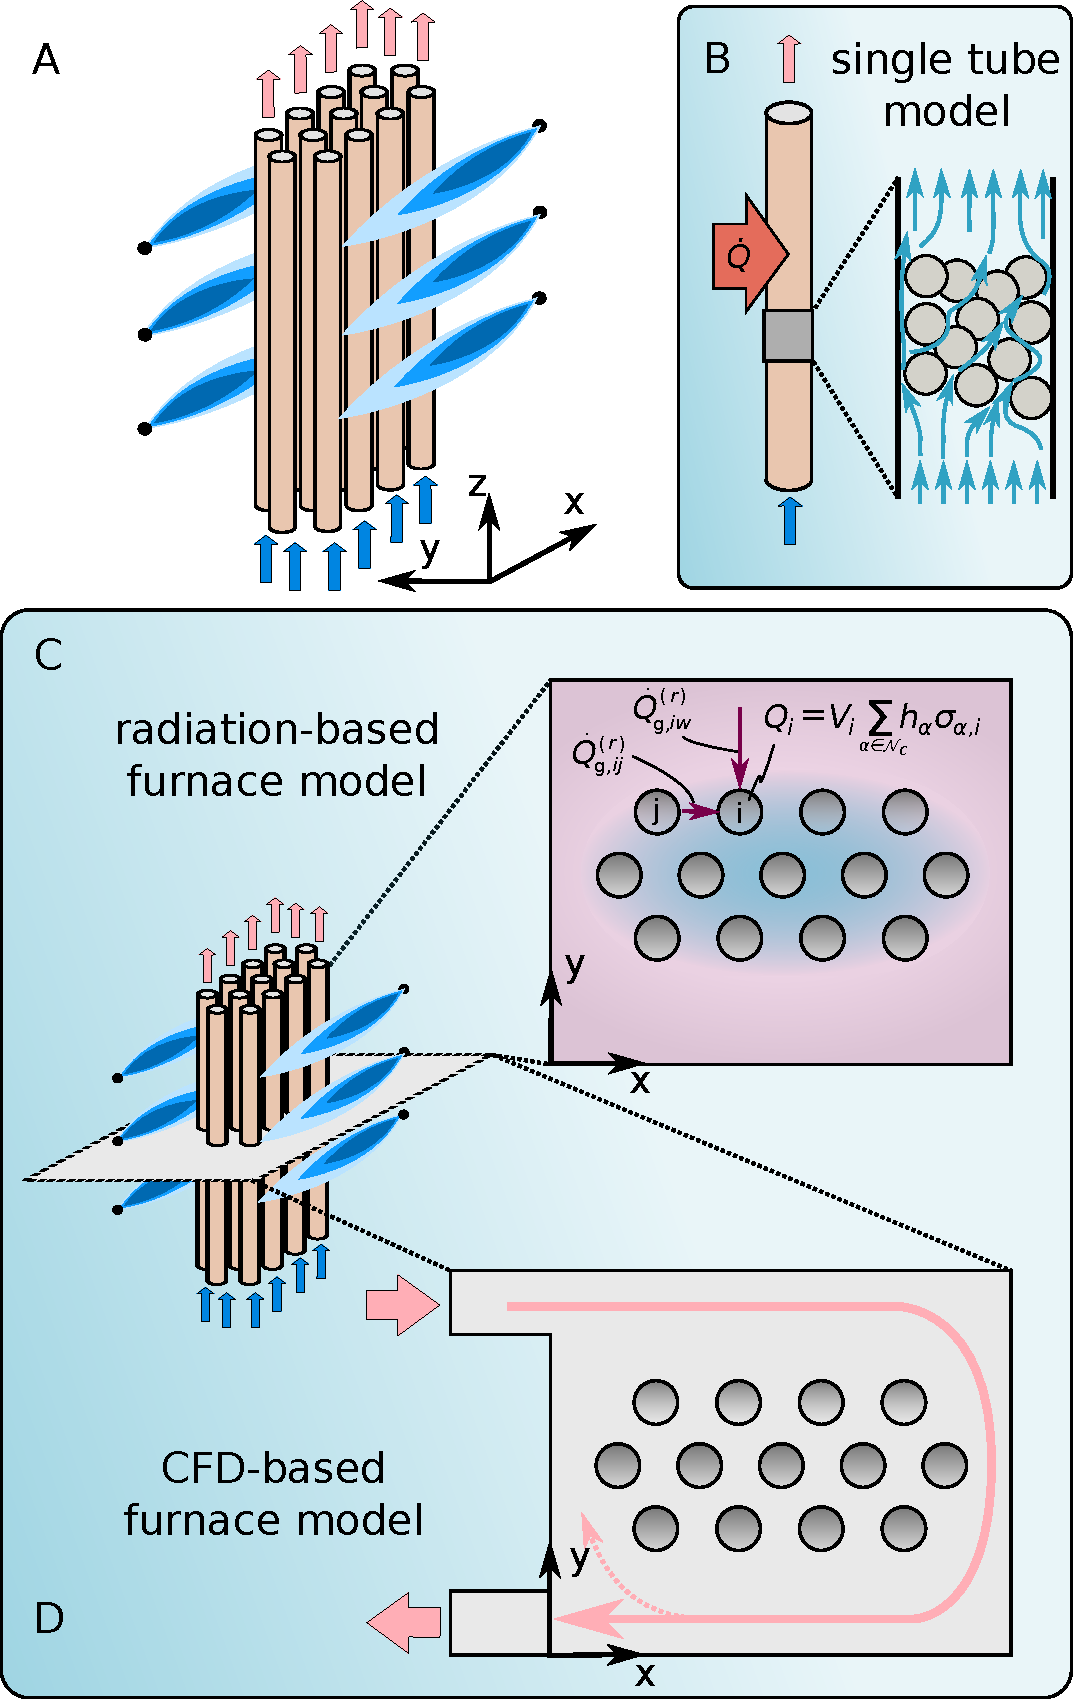
\includegraphics[width=85mm]{sources/figure1/MSR_modeling_approach.pdf}
%\caption{Sketch of a side-fired tube bundle furnace (A) and three different models: the single tube model (B), the radiation-based furnace model (C) and the CFD-based furnace model (D).}%
%\label{fig:MSR_model_sketch}
\end{figure}
\efloatseparator
%%

\begin{figure}
	\centering
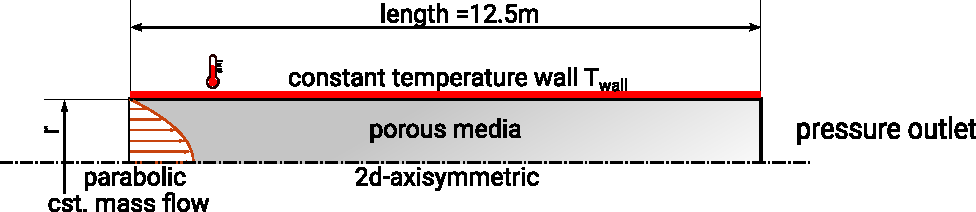
\includegraphics[width=85mm]{sources/figure2/singleTubeSketch.pdf}
%	\caption{Schematic representation of the flow simulations domain for a single reforming tube.}%
%	\label{f:singleTube_setupSketch}
\end{figure}
\efloatseparator
%%

\begin{figure}
\centering
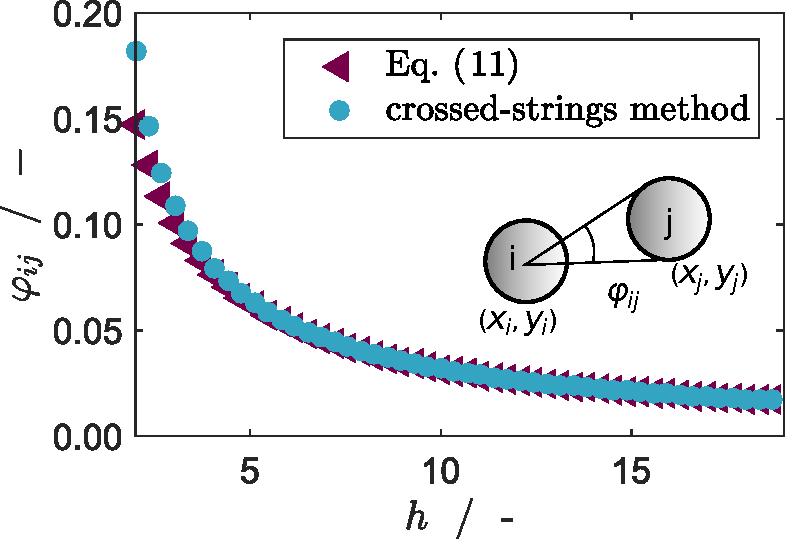
\includegraphics[width=85mm]{sources/figure3/view_factor_comparison.pdf}
%\caption{View factors between tube $i$ and $j$: \gls{viewfactor}[ij] calculated using~\autoref{eq:view_factor_calculation} (red triangles) and compared with the crossed-strings method (blue circles) versus the distance ratio $\gls{distancefactor}:=\gls{distancestubes}[ij]/\gls{radius}$.}
%\label{fig:bundle_model_sketch_view}
\end{figure}
\efloatseparator
%%

\begin{figure}
	\centering
	\def\svgwidth{85mm}
	\input{sources/figure4/cfdCaseSketches.pdf_tex}
%	\caption{
%		Schematic representation of the furnace geometry and four canonical tube arrangements assessed in the parameter study.
%		Configurations: line~(\gls{caseA}), staggered~(\gls{caseB}), aligned~(\gls{caseC}), and rectangle~(\gls{caseD}).
%	}%
%	\label{f:optGeometrySchematics}
\end{figure}
\efloatseparator
%%
\textwidth=180mm
\begin{figure}
	\centering
	\begin{tikzpicture}
    \begin{axis}[
			name=plot1,
	        width=85mm,
			height=60mm,     % size of the image
	        grid = major,
	     	grid style={line width=.1pt, draw=gray!10},	     	
	        xmin=800,     % start the diagram at this x-coordinate
	        xmax=1800,    % end   the diagram at this x-coordinate	    
	        xtick={800,1050,...,1800},
	        ymin=0.001,     % start the diagram at this y-coordinate
	        ymax=1,   % end   the diagram at this y-coordinate
	        ytick distance=0.2,
			minor y tick num=1,
			minor x tick num=4,
%	        ymode=log,
	        axis background/.style={fill=white},
			xlabel={$\gls{temp}_{\mathrm{wall}}$ / \si{\kelvin}},
			ylabel={$\gls{yield}[\ce{CO}]$ / --},
	        tick align=inside,
	        cycle list name=mpiovgucolors,
	        smooth,
        ]
   
      % import the correct data from a CSV file
		\addplot table[x=WallTemperature,y=Yield_CO_outlet,col sep=comma] {sources/figure5/SMR_C_TubeRad_008.csv};	
			\label{p:smr8}
		\addplot table[x=WallTemperature,y=Yield_CO_outlet,col sep=comma] {sources/figure5/SMR_C_TubeRad_007.csv};
			\label{p:smr7}
%		\addplot table[x=WallTemperature,y=Yield_CO_outlet,col sep=comma] {sources/figure5/SMR_C_TubeRad_006.csv};
%			\label{p:smr6}
		\addplot table[x=WallTemperature,y=Yield_CO_outlet,col sep=comma] {sources/figure5/SMR_C_TubeRad_0063.csv};
			\label{p:smr63}
		\addplot table[x=WallTemperature,y=Yield_CO_outlet,col sep=comma] {sources/figure5/SMR_C_TubeRad_005.csv};
			\label{p:smr5}
		\addplot table[x=WallTemperature,y=Yield_CO_outlet,col sep=comma] {sources/figure5/SMR_C_TubeRad_004.csv};
			\label{p:smr4}
		\addplot table[x=WallTemperature,y=Yield_CO_outlet,col sep=comma] {sources/figure5/SMR_C_TubeRad_003.csv};
			\label{p:smr3}
		\addplot table[x=WallTemperature,y=Yield_CO_outlet,col sep=comma] {sources/figure5/SMR_C_TubeRad_002.csv};		
			\label{p:smr2}
		\addplot table[x=WallTemperature,y=Yield_CO_outlet,col sep=comma] {sources/figure5/SMR_C_TubeRad_001.csv};
			\label{p:smr1}
		\coordinate (c1) at (rel axis cs:0,1);
	\end{axis};
	\begin{axis}[
		name=plot1detail,
		width=30mm,
		height=40mm,
		grid = both,
		grid style={line width=.1pt, draw=gray!10},	     	
		xmin=1150,     % start the diagram at this x-coordinate
		xmax=1250,    % end   the diagram at this x-coordinate	    
		xtick={1150,1250},
		minor x tick num=1,
		ymin=0.58,     % start the diagram at this y-coordinate
		ymax=0.66,   % end   the diagram at this y-coordinate
		ytick distance=0.05,
		minor y tick num=4,
		%	        ymode=log,
		axis background/.style={fill=white},
	%    xlabel=Wall temperature ($K$),
	%    ylabel=$Y_{\ce{CO}}$ (-),
		tick align=inside,
		ticklabel style = {font=\scriptsize},
		cycle list name=mpiovgucolors,    
	%    legend pos=outer north east,
    	xshift=45mm,yshift=8mm % <-
		]
			\addplot table[x=WallTemperature,y=Yield_CO_outlet,col sep=comma] {sources/figure5/SMR_C_TubeRad_008.csv};	
			\addplot table[x=WallTemperature,y=Yield_CO_outlet,col sep=comma] {sources/figure5/SMR_C_TubeRad_007.csv};
%			\addplot table[x=WallTemperature,y=Yield_CO_outlet,col sep=comma] {sources/figure5/SMR_C_TubeRad_006.csv};
			\addplot table[x=WallTemperature,y=Yield_CO_outlet,col sep=comma] {sources/figure5/SMR_C_TubeRad_0063.csv};
			\addplot table[x=WallTemperature,y=Yield_CO_outlet,col sep=comma] {sources/figure5/SMR_C_TubeRad_005.csv};
			\addplot table[x=WallTemperature,y=Yield_CO_outlet,col sep=comma] {sources/figure5/SMR_C_TubeRad_004.csv};
			\addplot table[x=WallTemperature,y=Yield_CO_outlet,col sep=comma] {sources/figure5/SMR_C_TubeRad_003.csv};
			\addplot table[x=WallTemperature,y=Yield_CO_outlet,col sep=comma] {sources/figure5/SMR_C_TubeRad_002.csv};		
			\addplot table[x=WallTemperature,y=Yield_CO_outlet,col sep=comma] {sources/figure5/SMR_C_TubeRad_001.csv};
	\end{axis};%
	%
	\begin{axis}[
		name=plot2,
		at={($(plot1.east)+(4pc,0)$)},
		anchor=west,
		width=85mm,
		height=60mm,
		grid = major,
		grid style={line width=.1pt, draw=gray!10},	     	
		xmin=800,     % start the diagram at this x-coordinate
		xmax=1800,    % end   the diagram at this x-coordinate	    
		xtick={800,1050,...,1800},
		minor x tick num=4,
		ymin=0,     % start the diagram at this y-coordinate
		ymax=70,   % end   the diagram at this y-coordinate
		%axis background/.style={fill=white},
		xlabel={$\gls{temp}_{\mathrm{wall}}$ / \si{\kelvin}},
		ylabel={$\gls{heatflux}[\mathrm{wall}]$ / \si{\kilo\watt\per\meter}},
		tick align=inside,
		cycle list name=mpiovgucolors,
		smooth,
	]

		% import the correct data from a CSV file
		\addplot table[x=WallTemperature,y expr=\thisrow{TotalHeatFlux}*-1/1000/12.5,col sep=comma] {sources/figure5/SMR_C_TubeRad_008.csv};
		\addplot table[x=WallTemperature,y expr=\thisrow{TotalHeatFlux}*-1/1000/12.5,col sep=comma] {sources/figure5/SMR_C_TubeRad_007.csv};
%		\addplot table[x=WallTemperature,y expr=\thisrow{TotalHeatFlux}*-1/1000/12.5,col sep=comma] {sources/figure5/SMR_C_TubeRad_006.csv};
		\addplot table[x=WallTemperature,y expr=\thisrow{TotalHeatFlux}*-1/1000/12.5,col sep=comma] {sources/figure5/SMR_C_TubeRad_0063.csv};
		\addplot table[x=WallTemperature,y expr=\thisrow{TotalHeatFlux}*-1/1000/12.5,col sep=comma] {sources/figure5/SMR_C_TubeRad_005.csv};
		\addplot table[x=WallTemperature,y expr=\thisrow{TotalHeatFlux}*-1/1000/12.5,col sep=comma] {sources/figure5/SMR_C_TubeRad_004.csv};
		\addplot table[x=WallTemperature,y expr=\thisrow{TotalHeatFlux}*-1/1000/12.5,col sep=comma] {sources/figure5/SMR_C_TubeRad_003.csv};
		\addplot table[x=WallTemperature,y expr=\thisrow{TotalHeatFlux}*-1/1000/12.5,col sep=comma] {sources/figure5/SMR_C_TubeRad_002.csv};		
		\addplot table[x=WallTemperature,y expr=\thisrow{TotalHeatFlux}*-1/1000/12.5,col sep=comma] {sources/figure5/SMR_C_TubeRad_001.csv};

		\coordinate (c2) at (rel axis cs:1,1);
	\end{axis};%
	\coordinate (c3) at ($(c1)!.5!(c2)$);

	\node[
		%at={($(plot1.south east)+(0.05\linewidth,-2cm)$)},
		below,
		%anchor=north,
		rectangle,draw=black,thin,
		] at (c3 |- current bounding box.south)
		{
			\begin{tabular}{rcccccccc}
				\gls{radius}/\si{\meter} &	0.01 & 0.02 & 0.03 & 0.04 & 0.05 & 0.063 & 0.07 & 0.08 \\
				&	\ref*{p:smr1} & \ref*{p:smr2} & \ref*{p:smr3} & \ref*{p:smr4} & \ref*{p:smr5} & \ref*{p:smr63} & \ref*{p:smr7} & \ref*{p:smr8} \\
			\end{tabular}
		};%
			
\end{tikzpicture}

%	\caption{
%		Yield of \ce{CO}, \gls{yield}[\ce{CO}] of a single reforming tube, and wall heat flux \gls{heatflux}[\mathrm{wall}] per meter of tube, as result of different wall temperatures $\gls{temp}_{\mathrm{wall}}$ and inner tube radii \gls{radius}.
%		The left graph contains a zoomed view of the curves at \SI{1200}{\kelvin} as overlayed subplot.
%	}%
%	\label{f:singleTube_heatFlux_yield}
\end{figure}
\efloatseparator
%%

\textwidth=85mm
\begin{figure}
\centering
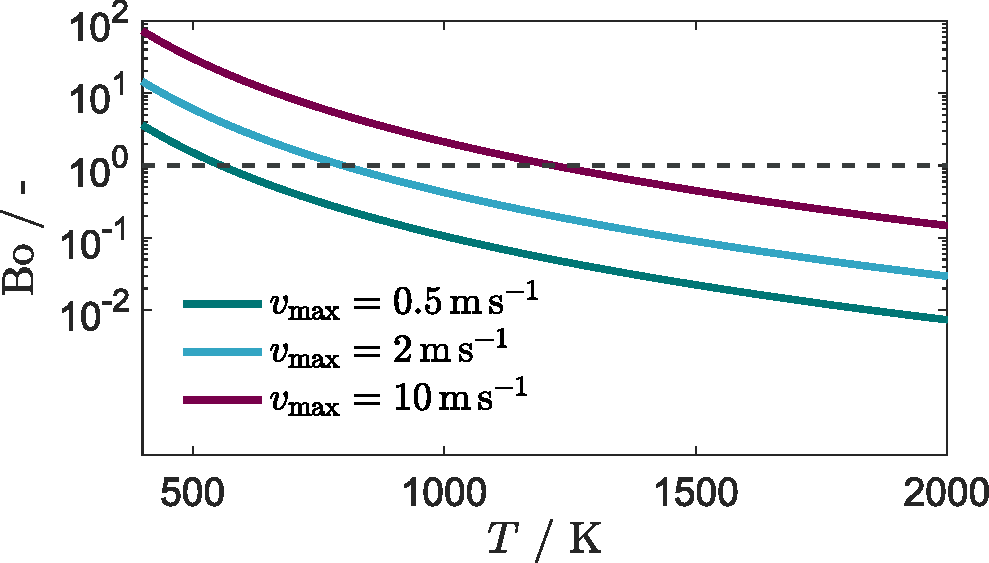
\includegraphics[width=85mm]{sources/figure6/Boltzmann_number.pdf}
%\caption{Boltzmann number \gls{boltzmannNumber} for three velocities $\gls{vel}_{\mathrm{max}} \in \{0.5, 2, 10\}\si{\meter\per\second}$.}%
%\label{fig:Boltzmann_number}
\end{figure}
\efloatseparator%
%%

\begin{figure}
	\centering
	

\begin{tikzpicture}
%\pgfplotsset{set layers=default};
\begin{axis}[
			width=80mm,
			height=60mm,     % size of the image
			grid = major,
			grid style={line width=.1pt, draw=gray!10},
			xmin=4000,     % start the diagram at this x-coordinate
			xmax=27000,    % end   the diagram at this x-coordinate
			ymin=87,     % start the diagram at this y-coordinate
			ymax=100,   % end   the diagram at this y-coordinate
			axis background/.style={fill=white},
			xlabel={\gls{heatfluxmean} / \si{\watt}},
			ylabel={\gls{heatfluxratio} / \si{\percent}},
			ylabel style={align=center},
			tick align=inside,
			minor x tick num=1,
			minor y tick num=1,
			cycle list name=mpiovgucolors2d,
%			scaled x ticks=true,
%			every x tick label/.append style={alias=XTick,inner xsep=0pt},
%			every x tick scale label/.style={at=(XTick.base east),anchor=base west},
			% change `clip mode' to `individual' to avoid unwanted clipping
			clip mode=individual,
			]

	%% import the correct data from a CSV file
	\addplot+[scatter=true,only marks, on layer=leins,point meta=explicit symbolic,scatter/@pre marker code/.style={/tikz/mark size=sqrt(\pgfplotspointmeta/\PI)*25}, scatter/@post marker code/.style={}]  table[x=HeatTransferMean(W),y=HeatFluxRatio (Rad/Total),meta=MassFlowPerTube (kg/s),col sep=semicolon] {sources/figure7/resultsCaseA-0.04.csv};
		\label{p:hfra4}
	\addplot+[scatter=true,only marks, on layer=leins,point meta=explicit symbolic,scatter/@pre marker code/.style={/tikz/mark size=sqrt(\pgfplotspointmeta/\PI)*25}, scatter/@post marker code/.style={}]  table[x=HeatTransferMean(W),y=HeatFluxRatio (Rad/Total),meta=MassFlowPerTube (kg/s),col sep=semicolon] {sources/figure7/resultsCaseA-0.063.csv};
		\label{p:hfra6}
	\addplot+[scatter=true,only marks, on layer=leins,point meta=explicit symbolic,scatter/@pre marker code/.style={/tikz/mark size=sqrt(\pgfplotspointmeta/\PI)*25}, scatter/@post marker code/.style={}]  table[x=HeatTransferMean(W),y=HeatFluxRatio (Rad/Total),meta=MassFlowPerTube (kg/s),col sep=semicolon] {sources/figure7/resultsCaseA-0.08.csv};
		\label{p:hfra8}
	\addplot+[scatter=true,only marks, on layer=lzwei,point meta=explicit symbolic,scatter/@pre marker code/.style={/tikz/mark size=sqrt(\pgfplotspointmeta/\PI)*25}, scatter/@post marker code/.style={}]  table[x=HeatTransferMean(W),y=HeatFluxRatio (Rad/Total),meta=MassFlowPerTube (kg/s),col sep=semicolon] {sources/figure7/resultsCaseB-0.04.csv};
		\label{p:hfrb4}
	\addplot+[scatter=true,only marks, on layer=lzwei,point meta=explicit symbolic,scatter/@pre marker code/.style={/tikz/mark size=sqrt(\pgfplotspointmeta/\PI)*25}, scatter/@post marker code/.style={}]  table[x=HeatTransferMean(W),y=HeatFluxRatio (Rad/Total),meta=MassFlowPerTube (kg/s),col sep=semicolon] {sources/figure7/resultsCaseB-0.063.csv};
		\label{p:hfrb6}
	\addplot+[scatter=true,only marks, on layer=lzwei,point meta=explicit symbolic,scatter/@pre marker code/.style={/tikz/mark size=sqrt(\pgfplotspointmeta/\PI)*25}, scatter/@post marker code/.style={}]  table[x=HeatTransferMean(W),y=HeatFluxRatio (Rad/Total),meta=MassFlowPerTube (kg/s),col sep=semicolon] {sources/figure7/resultsCaseB-0.08.csv};
		\label{p:hfrb8}
	\addplot+[scatter=true,only marks, on layer=ldrei,point meta=explicit symbolic,scatter/@pre marker code/.style={/tikz/mark size=sqrt(\pgfplotspointmeta/\PI)*25}, scatter/@post marker code/.style={}]  table[x=HeatTransferMean(W),y=HeatFluxRatio (Rad/Total),meta=MassFlowPerTube (kg/s),col sep=semicolon] {sources/figure7/resultsCaseC-0.04.csv};
		\label{p:hfrc4}
	\addplot+[scatter=true,only marks, on layer=ldrei,point meta=explicit symbolic,scatter/@pre marker code/.style={/tikz/mark size=sqrt(\pgfplotspointmeta/\PI)*25}, scatter/@post marker code/.style={}]  table[x=HeatTransferMean(W),y=HeatFluxRatio (Rad/Total),meta=MassFlowPerTube (kg/s),col sep=semicolon] {sources/figure7/resultsCaseC-0.063.csv};
		\label{p:hfrc6}
	\addplot+[scatter=true,only marks, on layer=ldrei,point meta=explicit symbolic,scatter/@pre marker code/.style={/tikz/mark size=sqrt(\pgfplotspointmeta/\PI)*25}, scatter/@post marker code/.style={}]  table[x=HeatTransferMean(W),y=HeatFluxRatio (Rad/Total),meta=MassFlowPerTube (kg/s),col sep=semicolon] {sources/figure7/resultsCaseC-0.08.csv};
		\label{p:hfrc8}
	\addplot+[scatter=true,only marks, on layer=lvier,point meta=explicit symbolic,scatter/@pre marker code/.style={/tikz/mark size=sqrt(\pgfplotspointmeta/\PI)*25}, scatter/@post marker code/.style={}]  table[x=HeatTransferMean(W),y=HeatFluxRatio (Rad/Total),meta=MassFlowPerTube (kg/s),col sep=semicolon] {sources/figure7/resultsCaseD-0.04.csv};
		\label{p:hfrd4}
	\addplot+[scatter=true,only marks, on layer=lvier,point meta=explicit symbolic,scatter/@pre marker code/.style={/tikz/mark size=sqrt(\pgfplotspointmeta/\PI)*25}, scatter/@post marker code/.style={}]  table[x=HeatTransferMean(W),y=HeatFluxRatio (Rad/Total),meta=MassFlowPerTube (kg/s),col sep=semicolon] {sources/figure7/resultsCaseD-0.063.csv};
		\label{p:hfrd6}
	\addplot+[scatter=true,only marks, on layer=lvier,point meta=explicit symbolic,scatter/@pre marker code/.style={/tikz/mark size=sqrt(\pgfplotspointmeta/\PI)*25}, scatter/@post marker code/.style={}]  table[x=HeatTransferMean(W),y=HeatFluxRatio (Rad/Total),meta=MassFlowPerTube (kg/s),col sep=semicolon] {sources/figure7/resultsCaseD-0.08.csv};
		\label{p:hfrd8}
			

	% Coordinates for the external legend
	\coordinate (zero) at (axis description cs:0.5,0);
	
	\draw[dashed] (2.5e4,94) .. controls (0.5e4,93.5)   .. (0.45e4,93);
	
	\node [anchor=west]at (0.75e4,89) {\scalebox{.6}{with tubes in flue gas stream}};
	
	\node [anchor=east]at (2.6e4,99) {\scalebox{.6}{mostly undisturbed flue gas flow}};
	
\end{axis}


\node[anchor=north,rectangle,draw=black,thin,inner sep=1pt] at (zero |- current bounding box.south) {
	\tikz{
		\node (L1) {
			\renewcommand\arraystretch{0.8}\setlength{\tabcolsep}{3pt}
			\begin{tabular}{rccc}
				\rotatebox{90}{~\rotatebox{-90}{\scriptsize \gls{radius} / \si{\meter}}}& \rotatebox{90}{\scalebox{.6}{0.04}} & \rotatebox{90}{\scalebox{.6}{0.063}} & \rotatebox{90}{\scalebox{.6}{0.08}} \\
%				\midrule
				\scriptsize  line 		& \ref*{p:hfra4} 	& \ref*{p:hfra6} 	& \ref*{p:hfra8} \\
				\scriptsize staggered 	& \ref*{p:hfrb4} 	& \ref*{p:hfrb6} 	& \ref*{p:hfrb8} \\
				\scriptsize aligned 		& \ref*{p:hfrc4} 	& \ref*{p:hfrc6} 	& \ref*{p:hfrc8} \\
				\scriptsize rectangle 	& \ref*{p:hfrd4} 	& \ref*{p:hfrd6} 	& \ref*{p:hfrd8} \\
			\end{tabular}
		};
		\node[right of=L1,xshift=1cm,anchor=west] {
			\tikz[]{
				\draw(0,0)--(0,1.5);
				\foreach \y/\ytext in {0/~,0.25/0.01,0.50/~,0.75/0.02,1.00/~,1.25/0.03,1.50/~}
				\draw(-2pt,\y)--(2pt,\y) node[right] {\tiny\ytext};
				
				\foreach \y/\ytext in {0/1.00pt,.25/1.41pt,.50/1.73pt,.75/1.99pt,1.00/2.23pt,1.25/2.44pt,1.50/2.64pt}
				\draw[black!40] (-6pt,\y) circle (\ytext);
				
				\node[anchor=south,rotate=90,inner sep=0pt] at (-15pt,0.75) {\scalebox{.6}{\gls{massflow} / \si{\kilogram\per\second\per{tube}}}}
			}
		};
	}
};

\end{tikzpicture}

%	\caption{
%		Radiative heat flux ratio \gls{heatfluxratio} in relation to the mean heat flux per tube~\gls{heatfluxmean}.
%		The symbol (and its color family) indicates the configuration of the data point.
%		Shades of the respective color indicate the inner tube radius~\gls{radius}.
%		The symbol size indicates the mass flow rate~\gls{massflow} of flue gas per reforming tube.
%	}%
%	\label{f:heatfluxratio}
\end{figure}
\efloatseparator%
%%
\textwidth=180mm
\begin{figure}
	\centering
	\usetikzlibrary{shapes.geometric, arrows,positioning,calc}
\begin{tikzpicture}
[
	inner sep=0pt,
 	every node/.style={inner sep=0,outer sep=0},
]

\node (n1a)  []                               {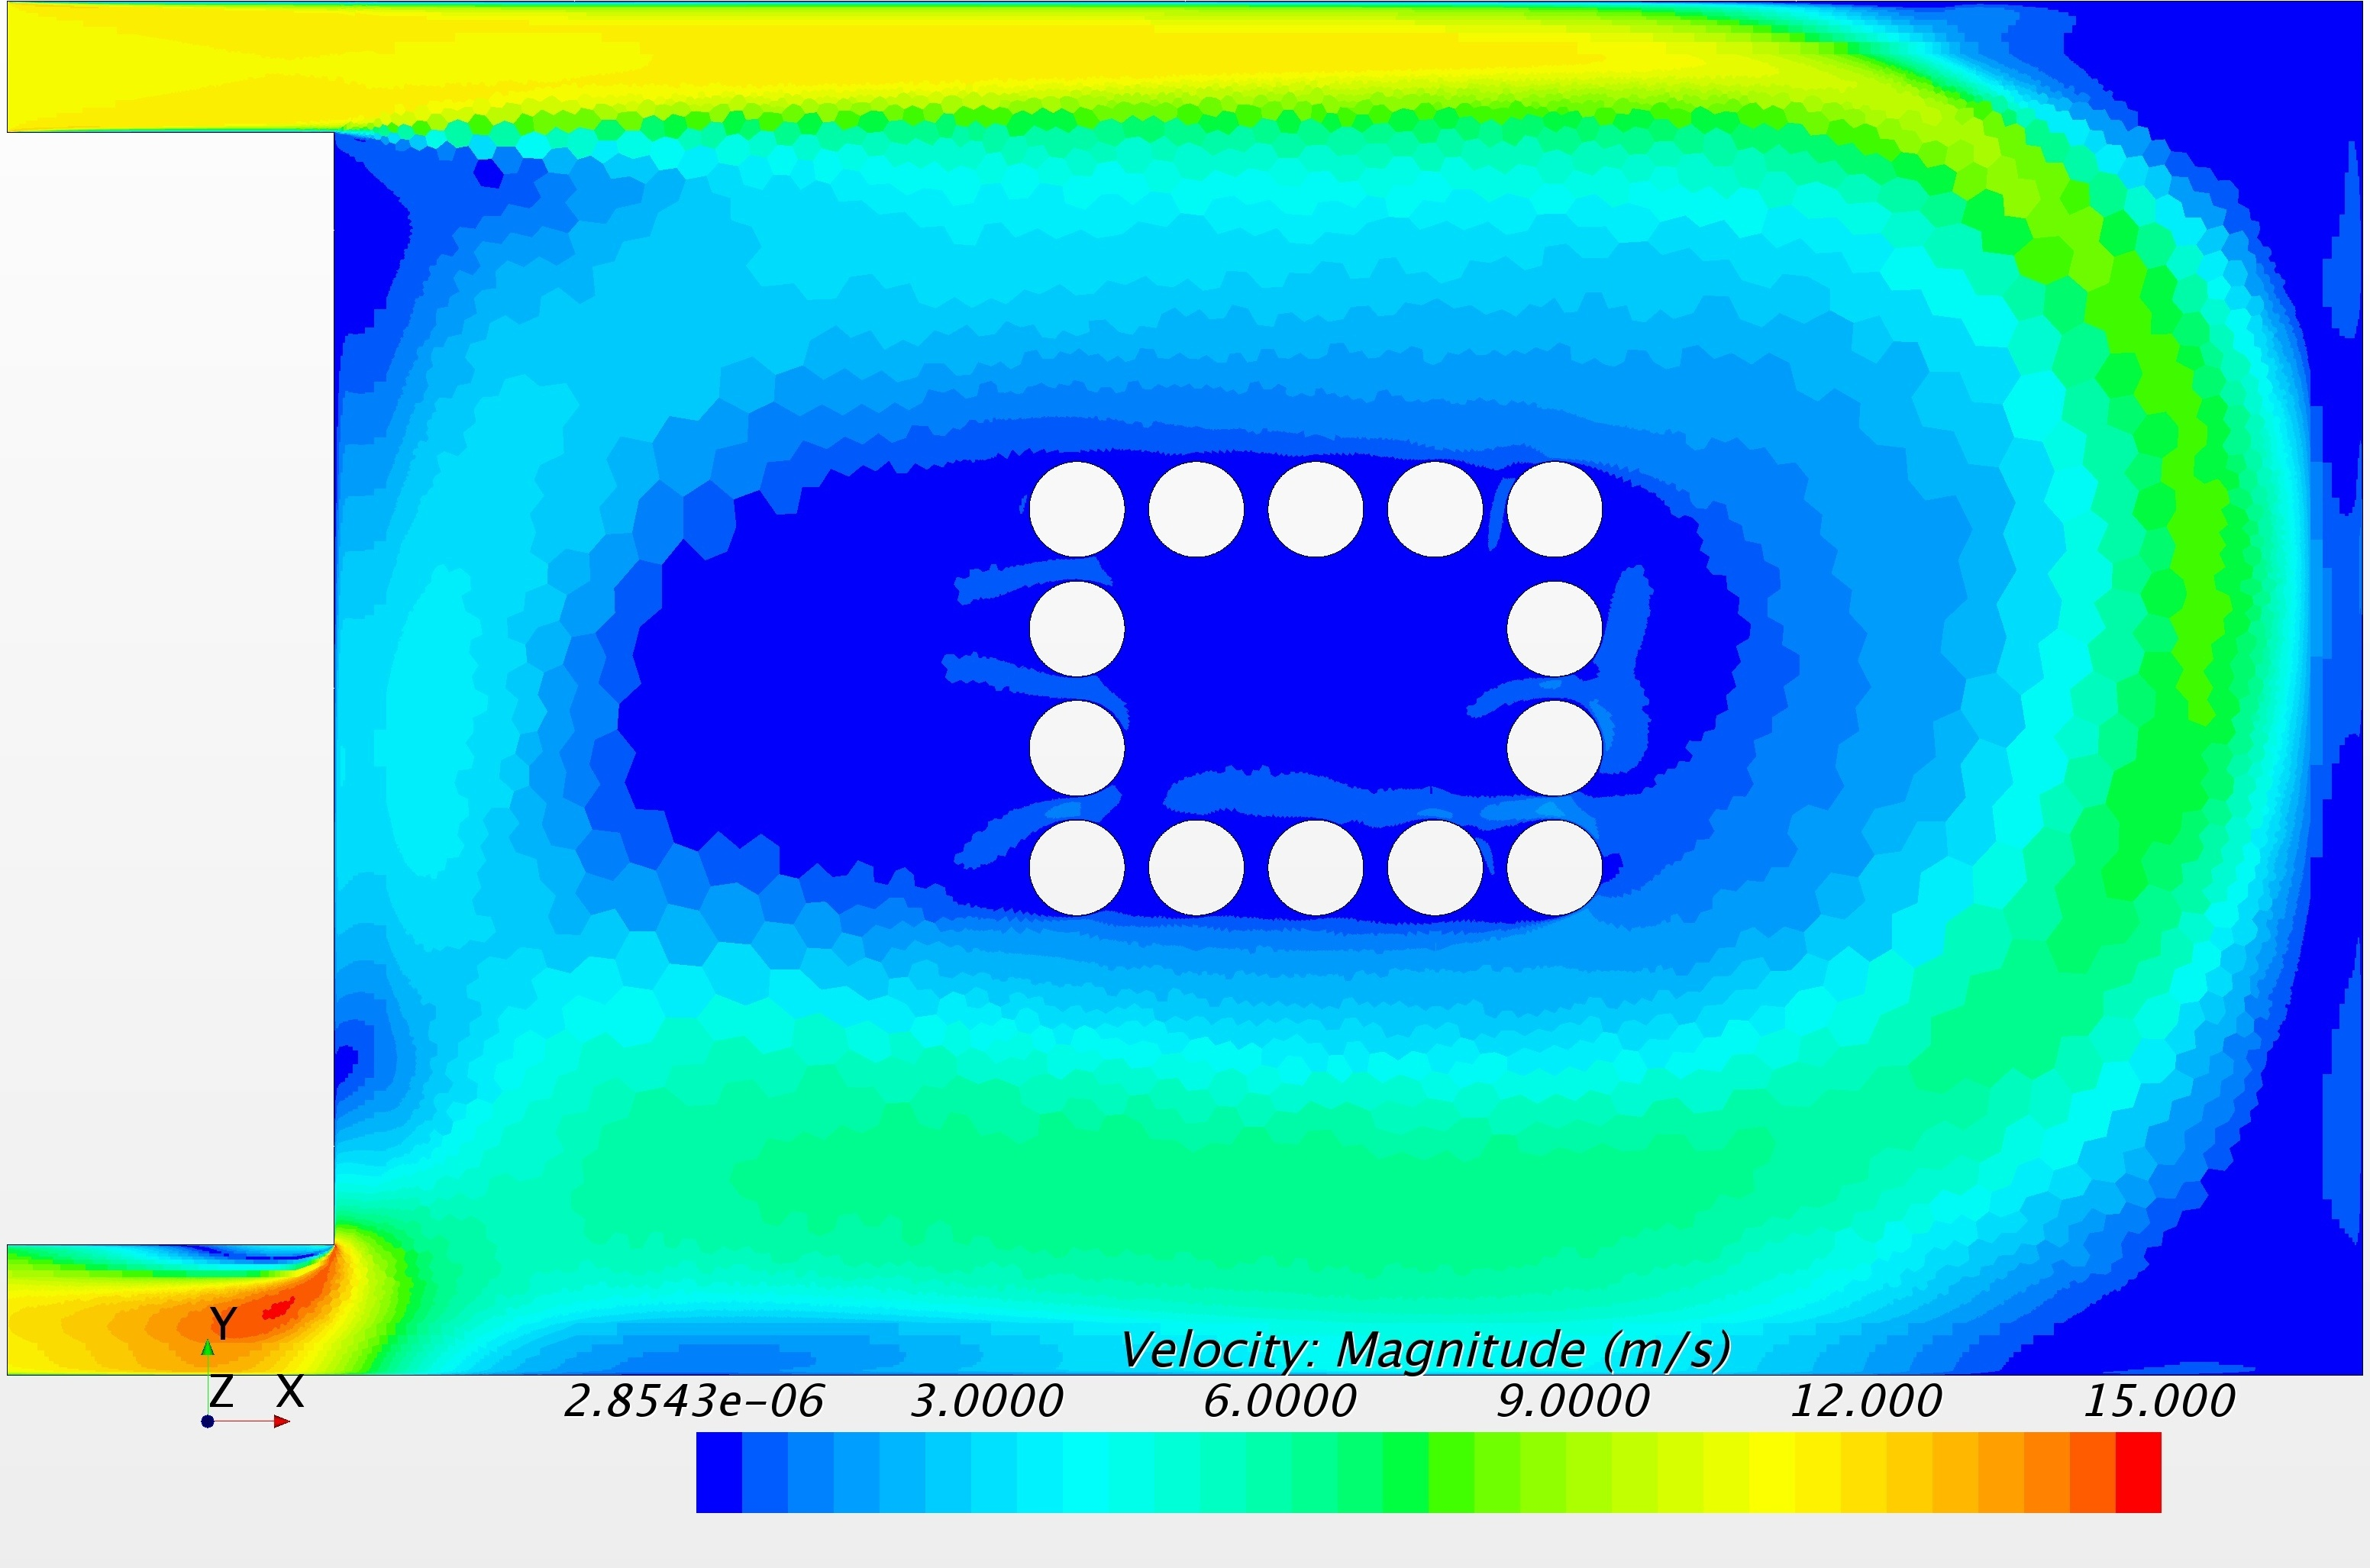
\includegraphics[height=3.8cm]{sources/figure8/c-vel_1.jpg}};
% \node (n2a)  [below=0cm of n1a,anchor=north]  {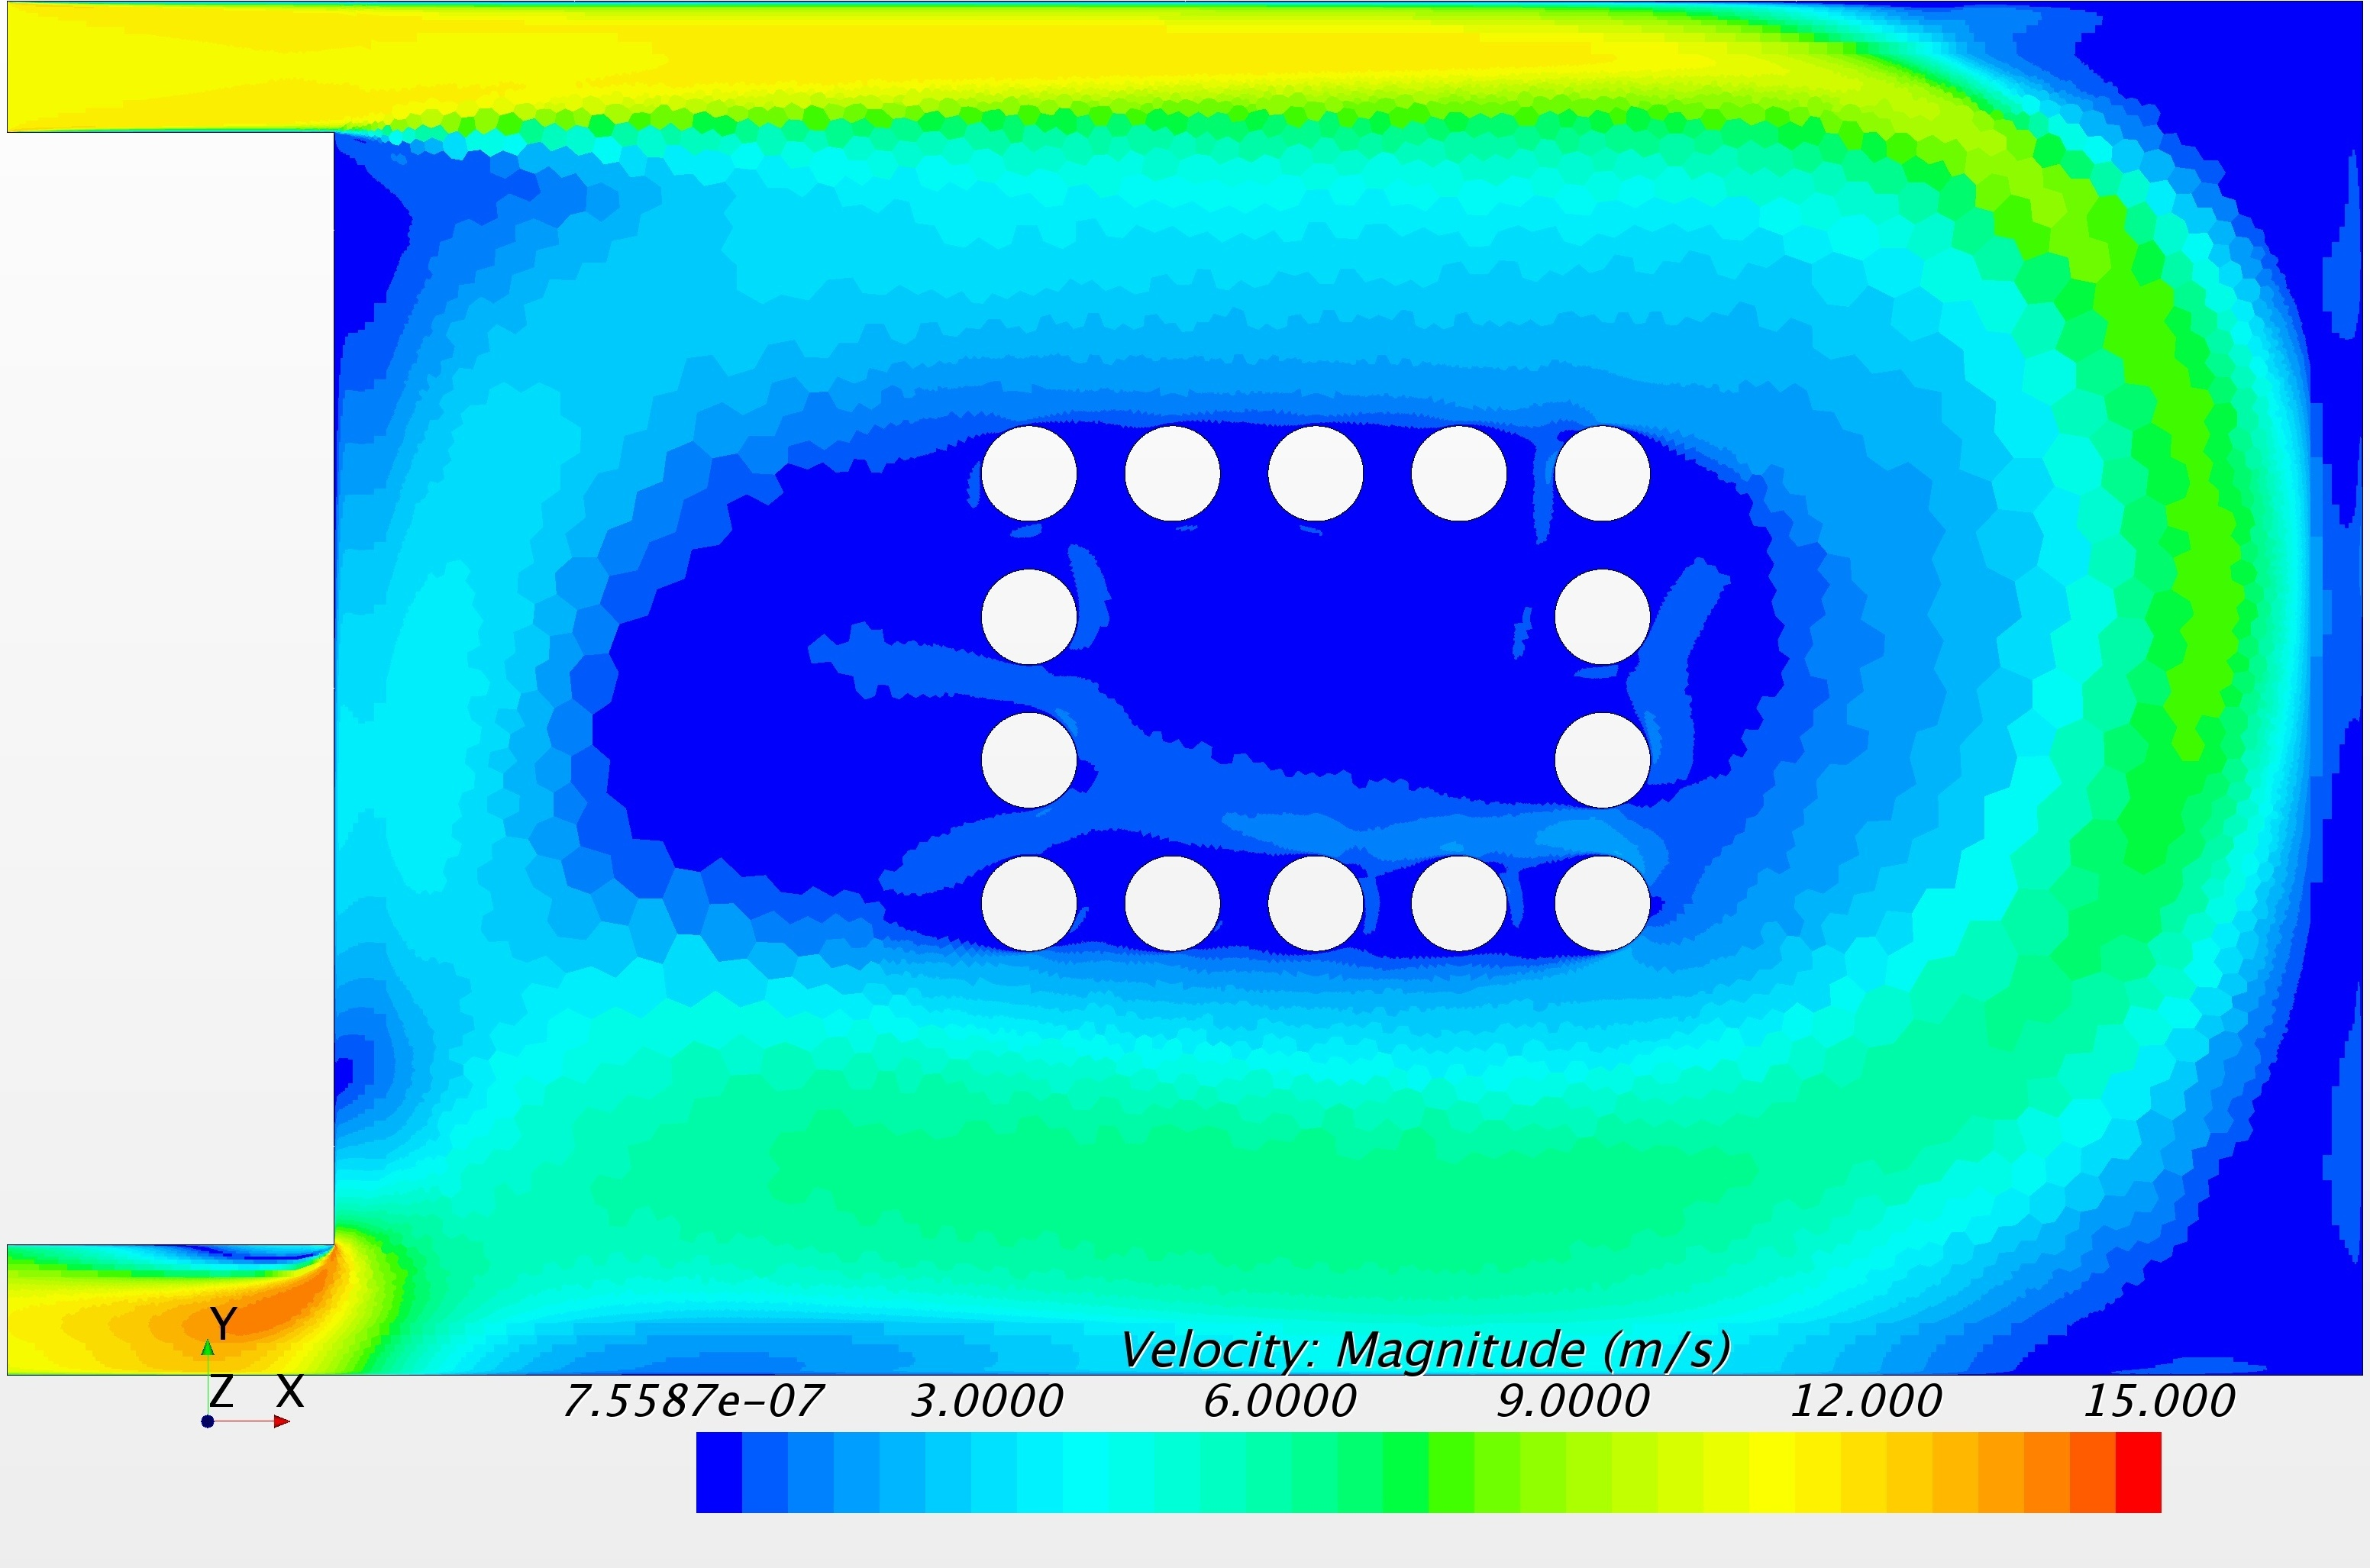
\includegraphics[height=3.8cm]{sources/figure8/c-vel_2.jpg}};
\node (n3a)  [below=0cm of n1a]               {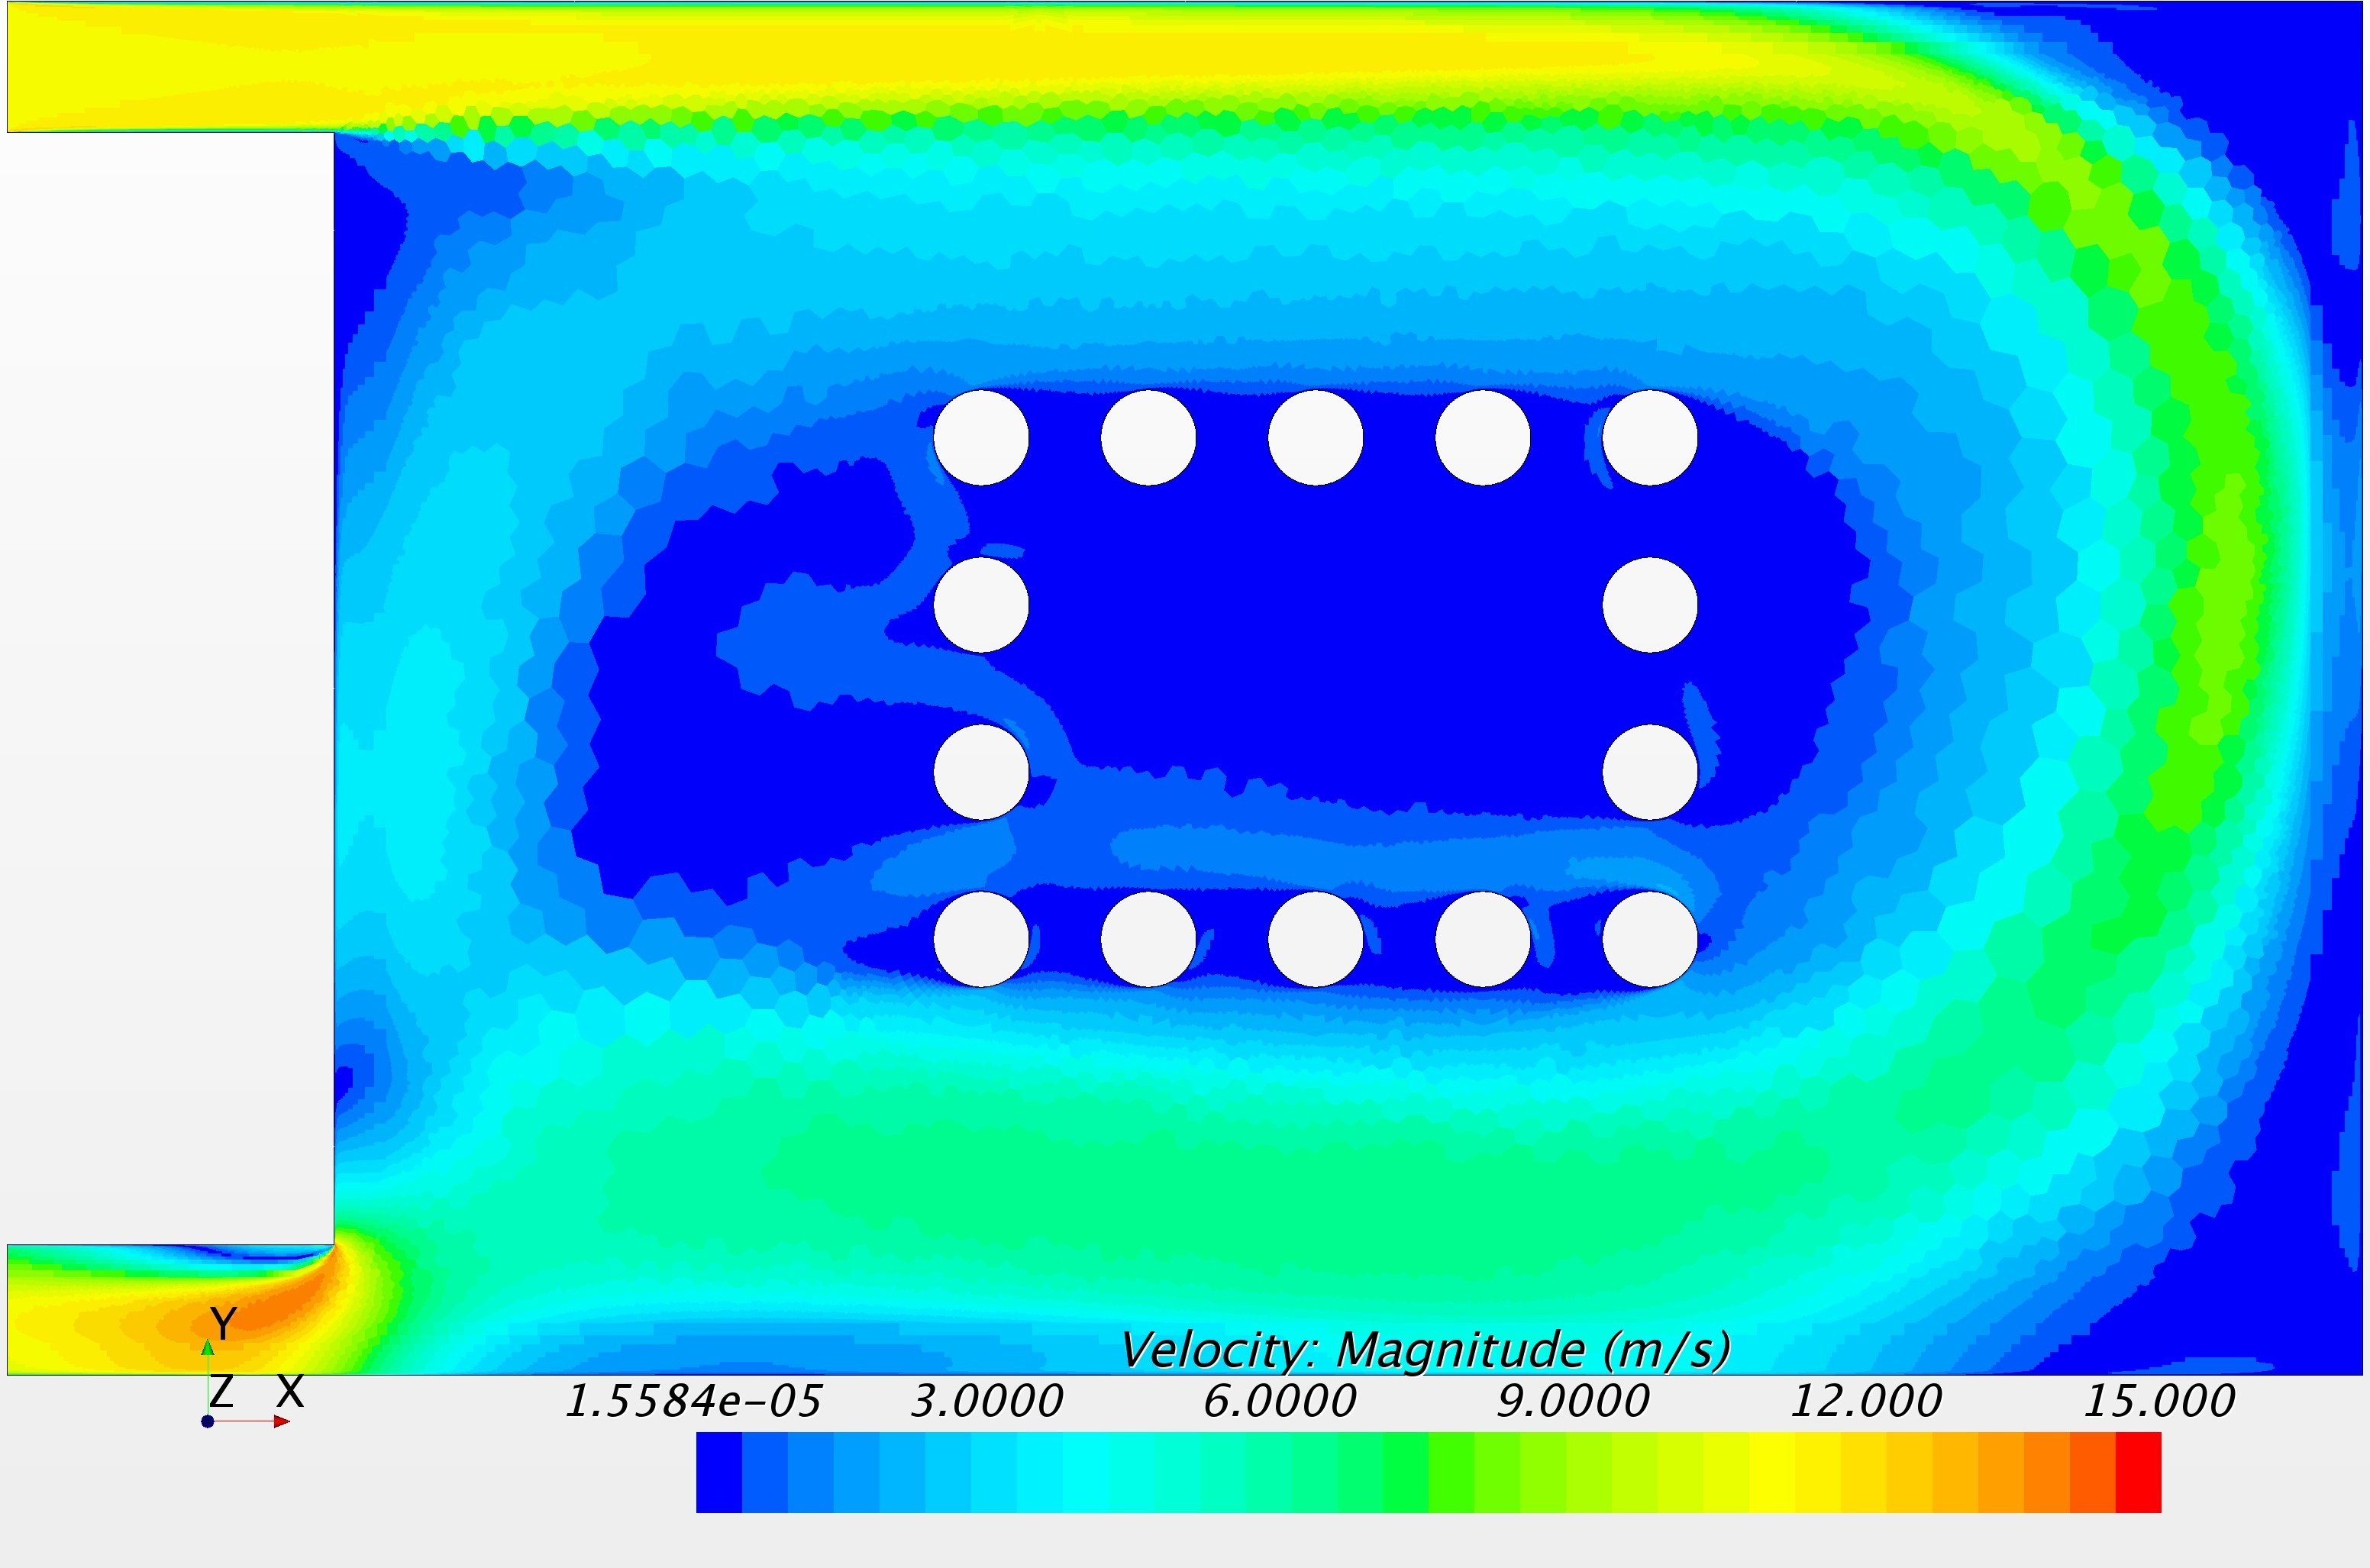
\includegraphics[height=3.8cm]{sources/figure8/c-vel_3.jpg}};
% \node (n4a)  [below=0cm of n3a,anchor=north]  {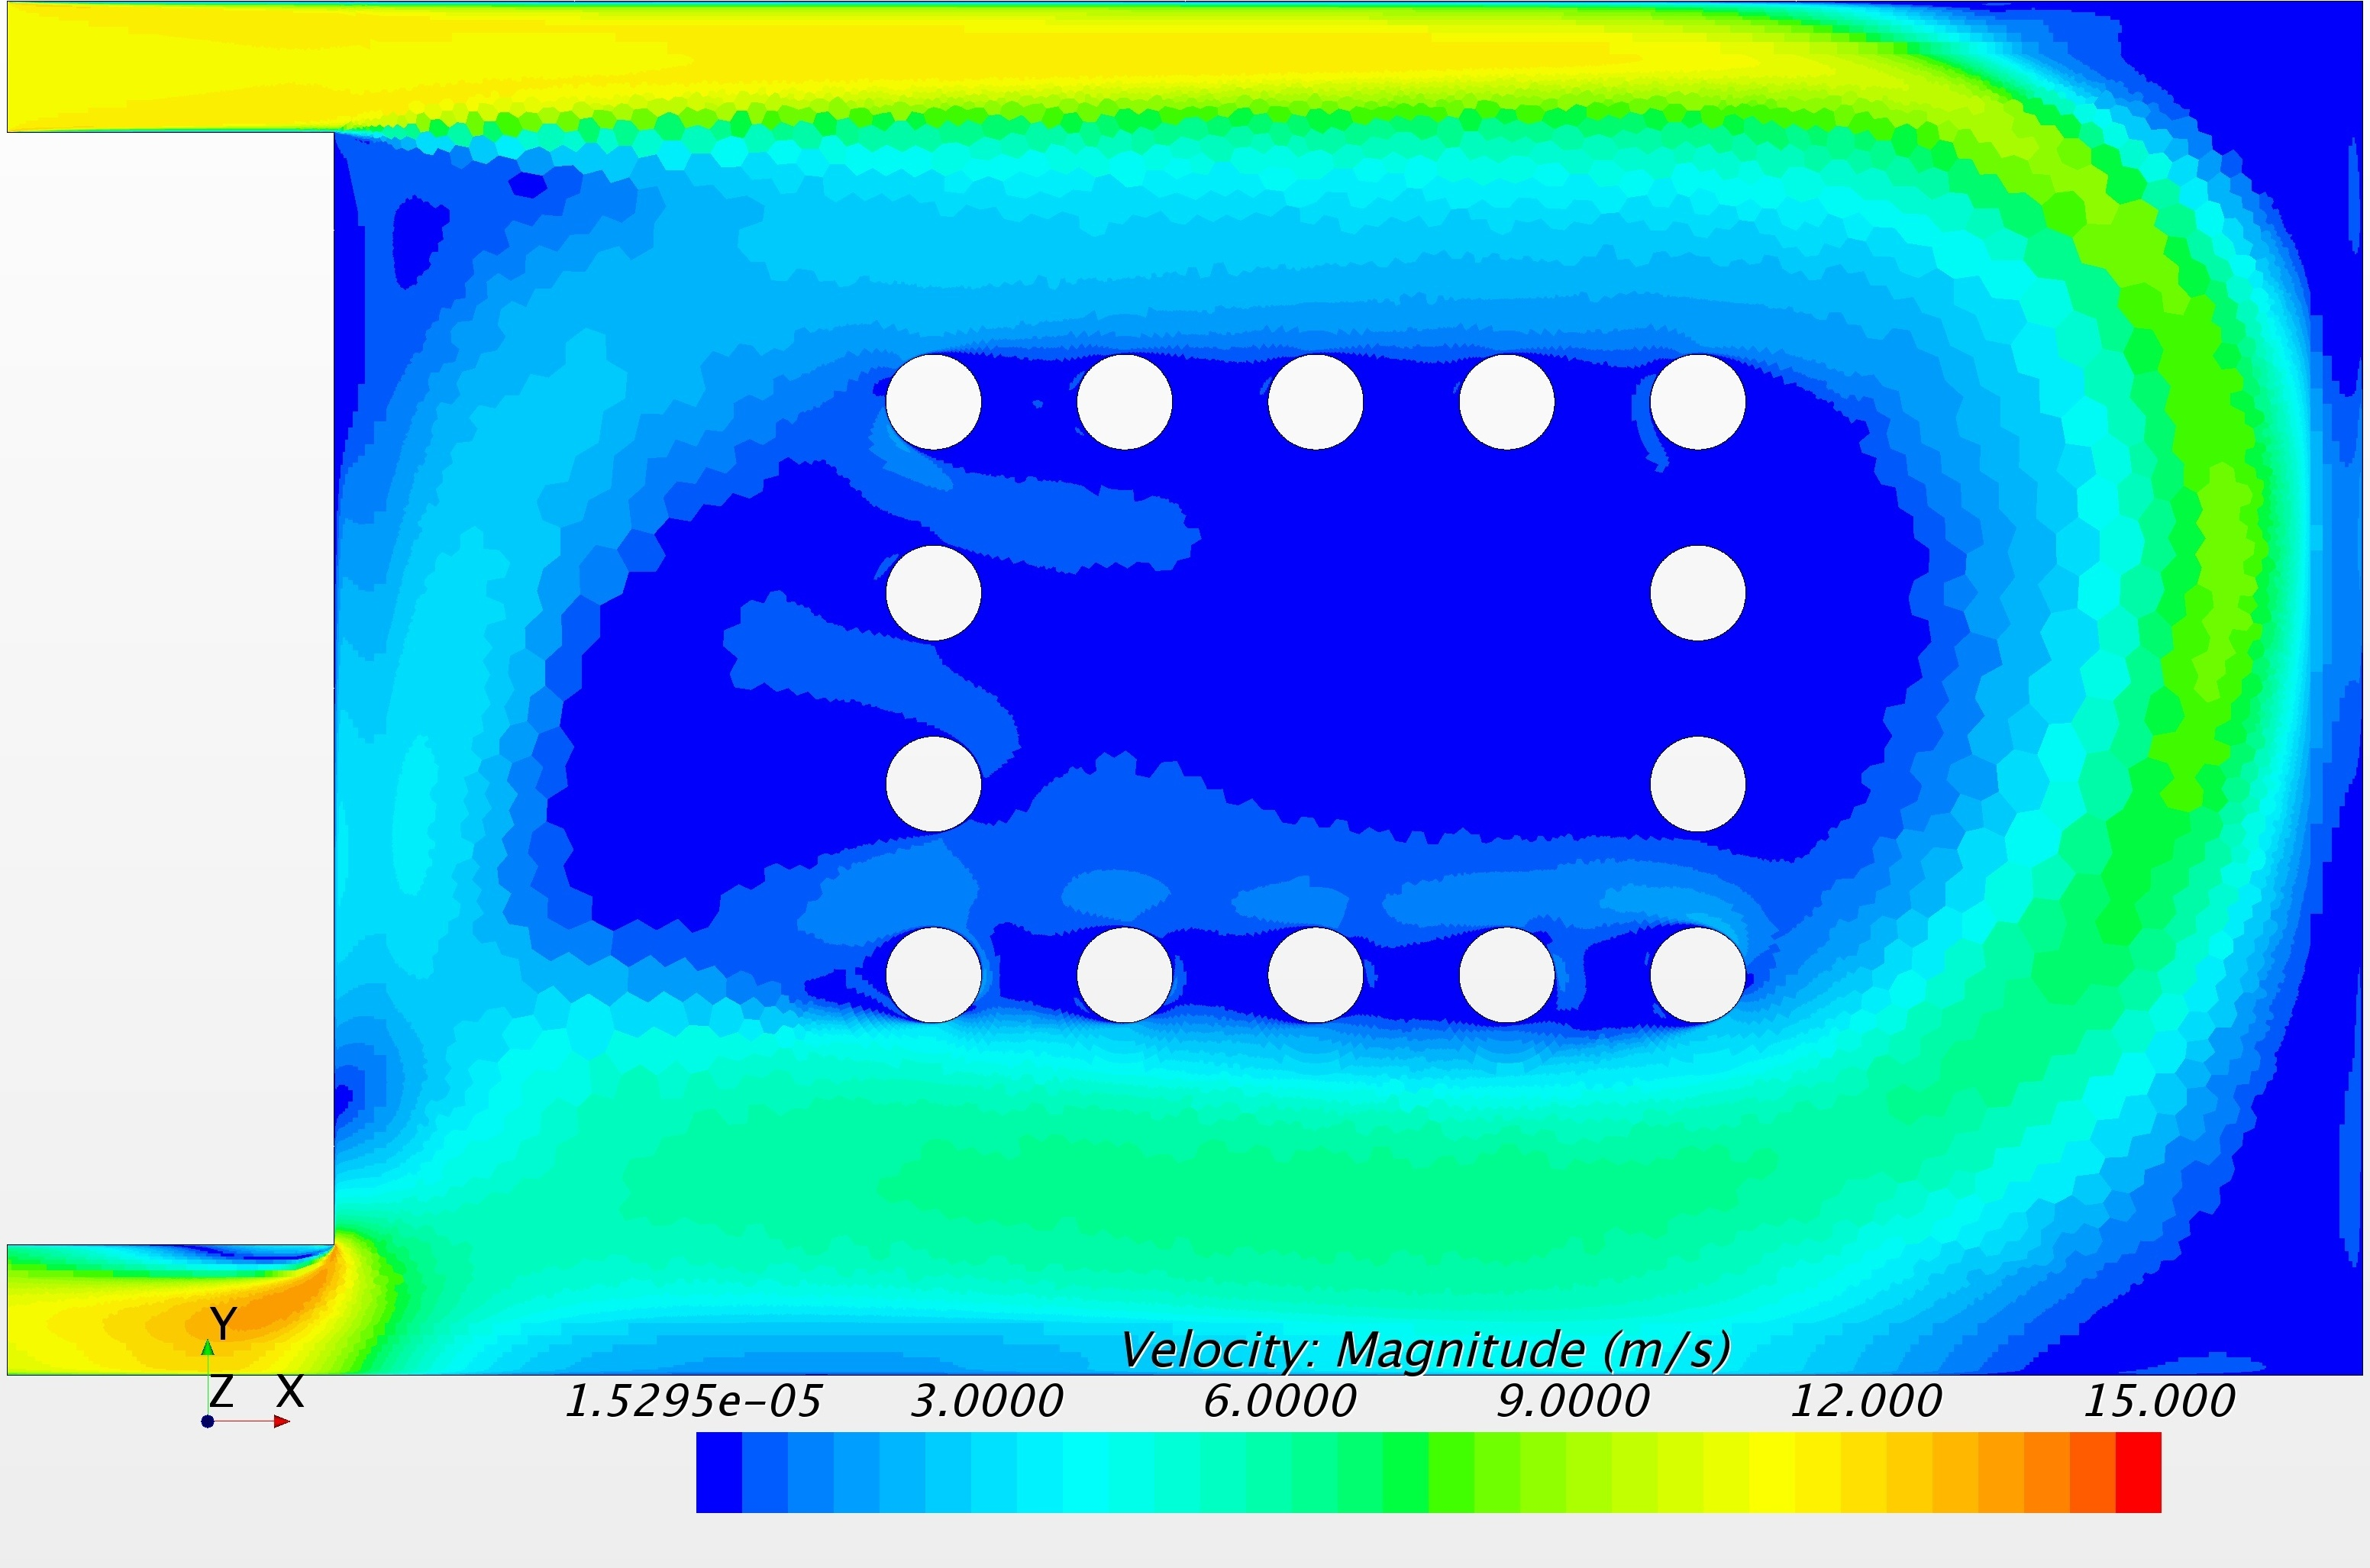
\includegraphics[height=3.8cm]{sources/figure8/c-vel_4.jpg}};
\node (n5a)  [below=0cm of n3a,anchor=north]  {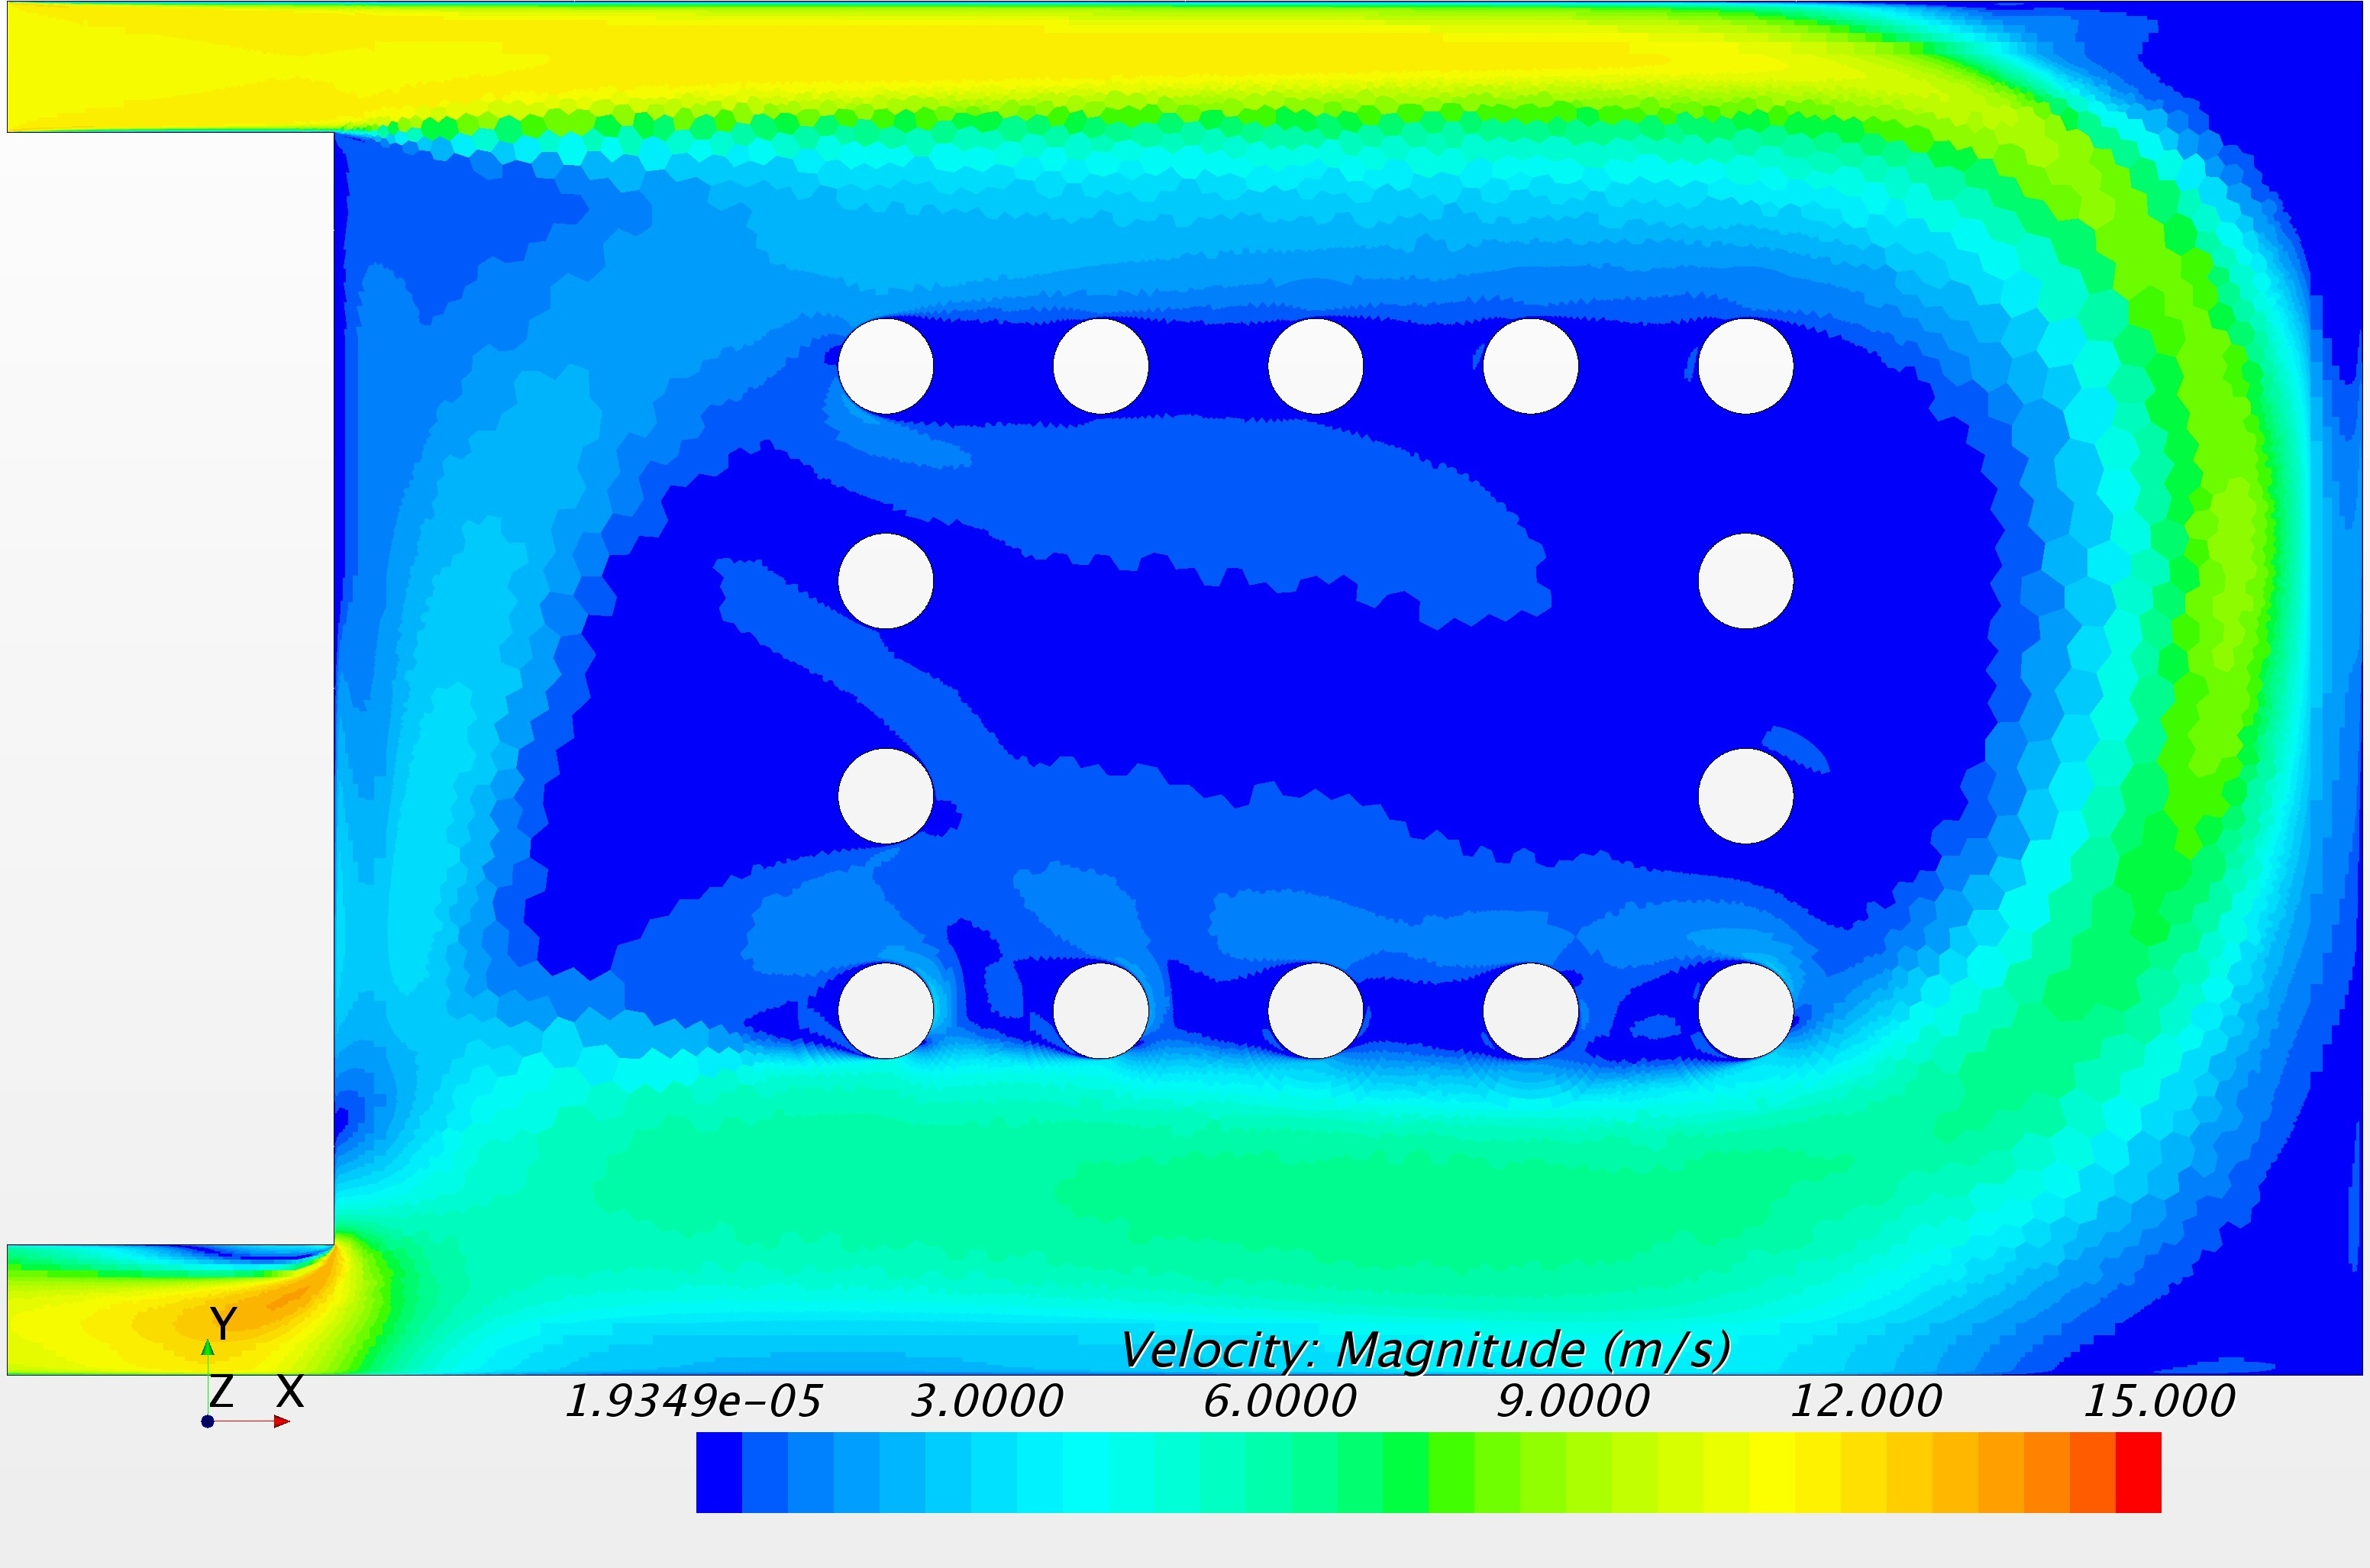
\includegraphics[height=3.8cm]{sources/figure8/c-vel_5.jpg}};
% \node (n6a)  [below=0cm of n5a,anchor=north]  {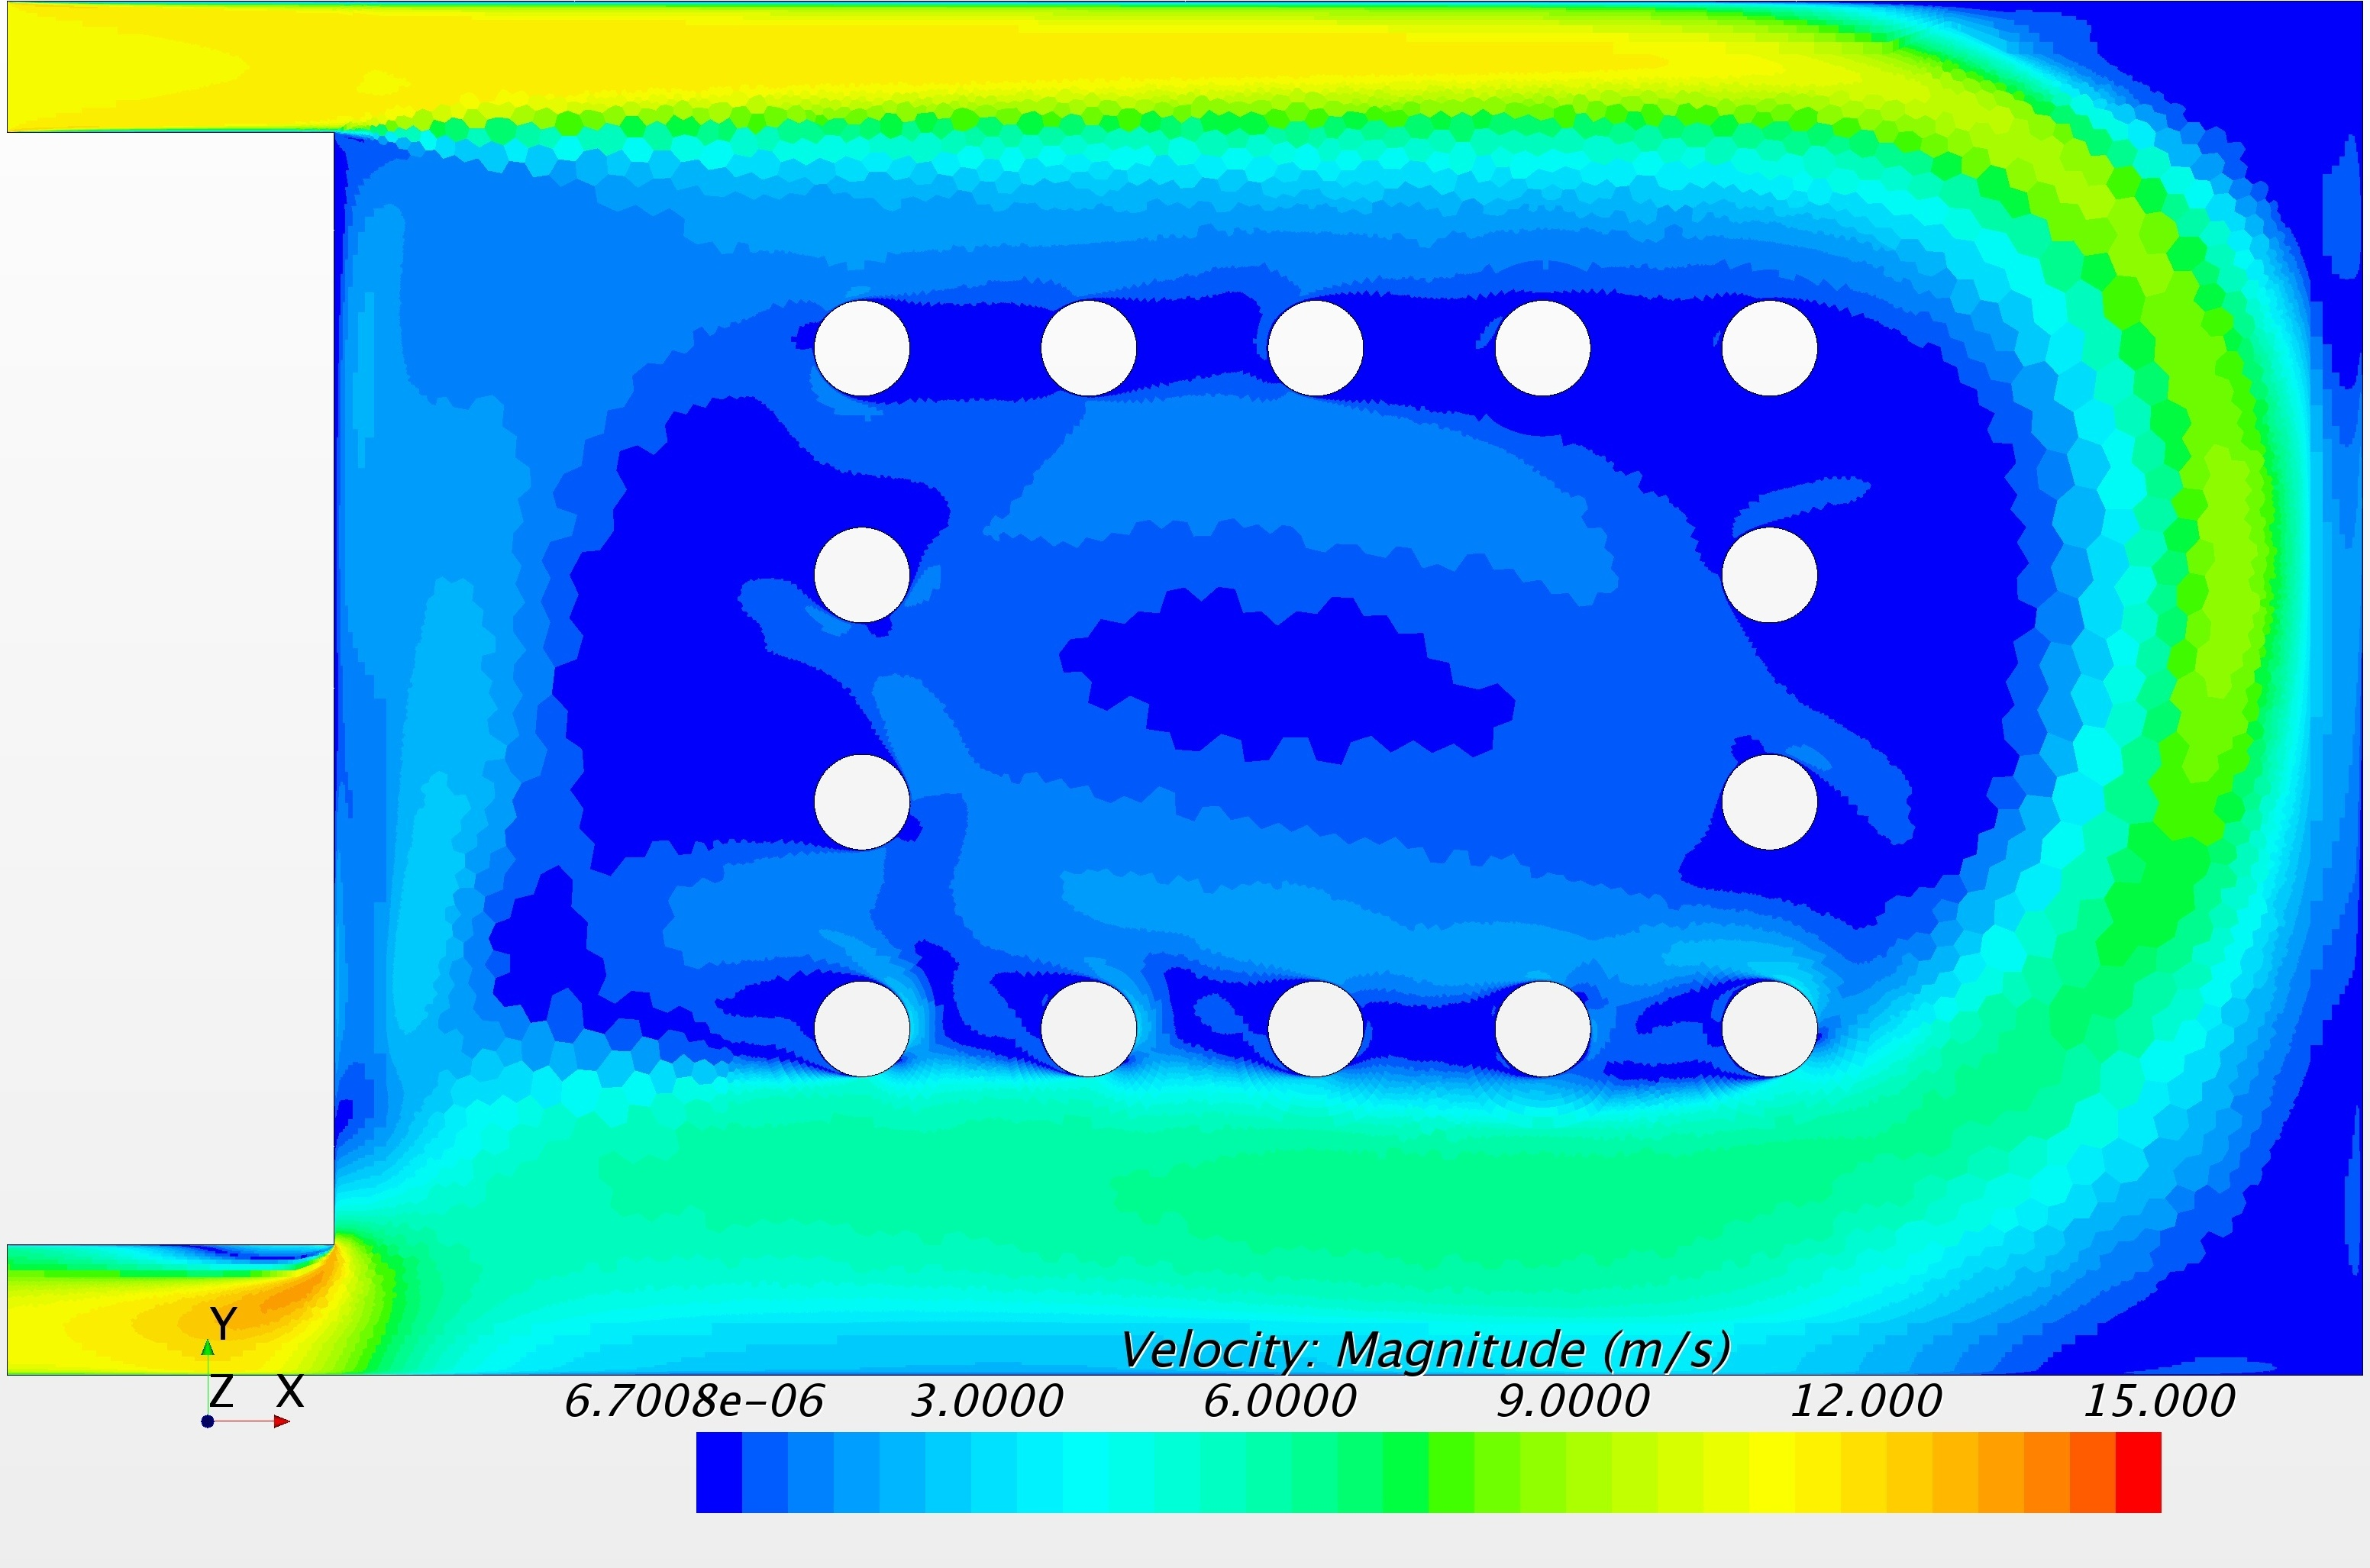
\includegraphics[height=3.8cm]{sources/figure8/c-vel_6.jpg}};
\node (n7a)  [below=0cm of n5a,anchor=north]  {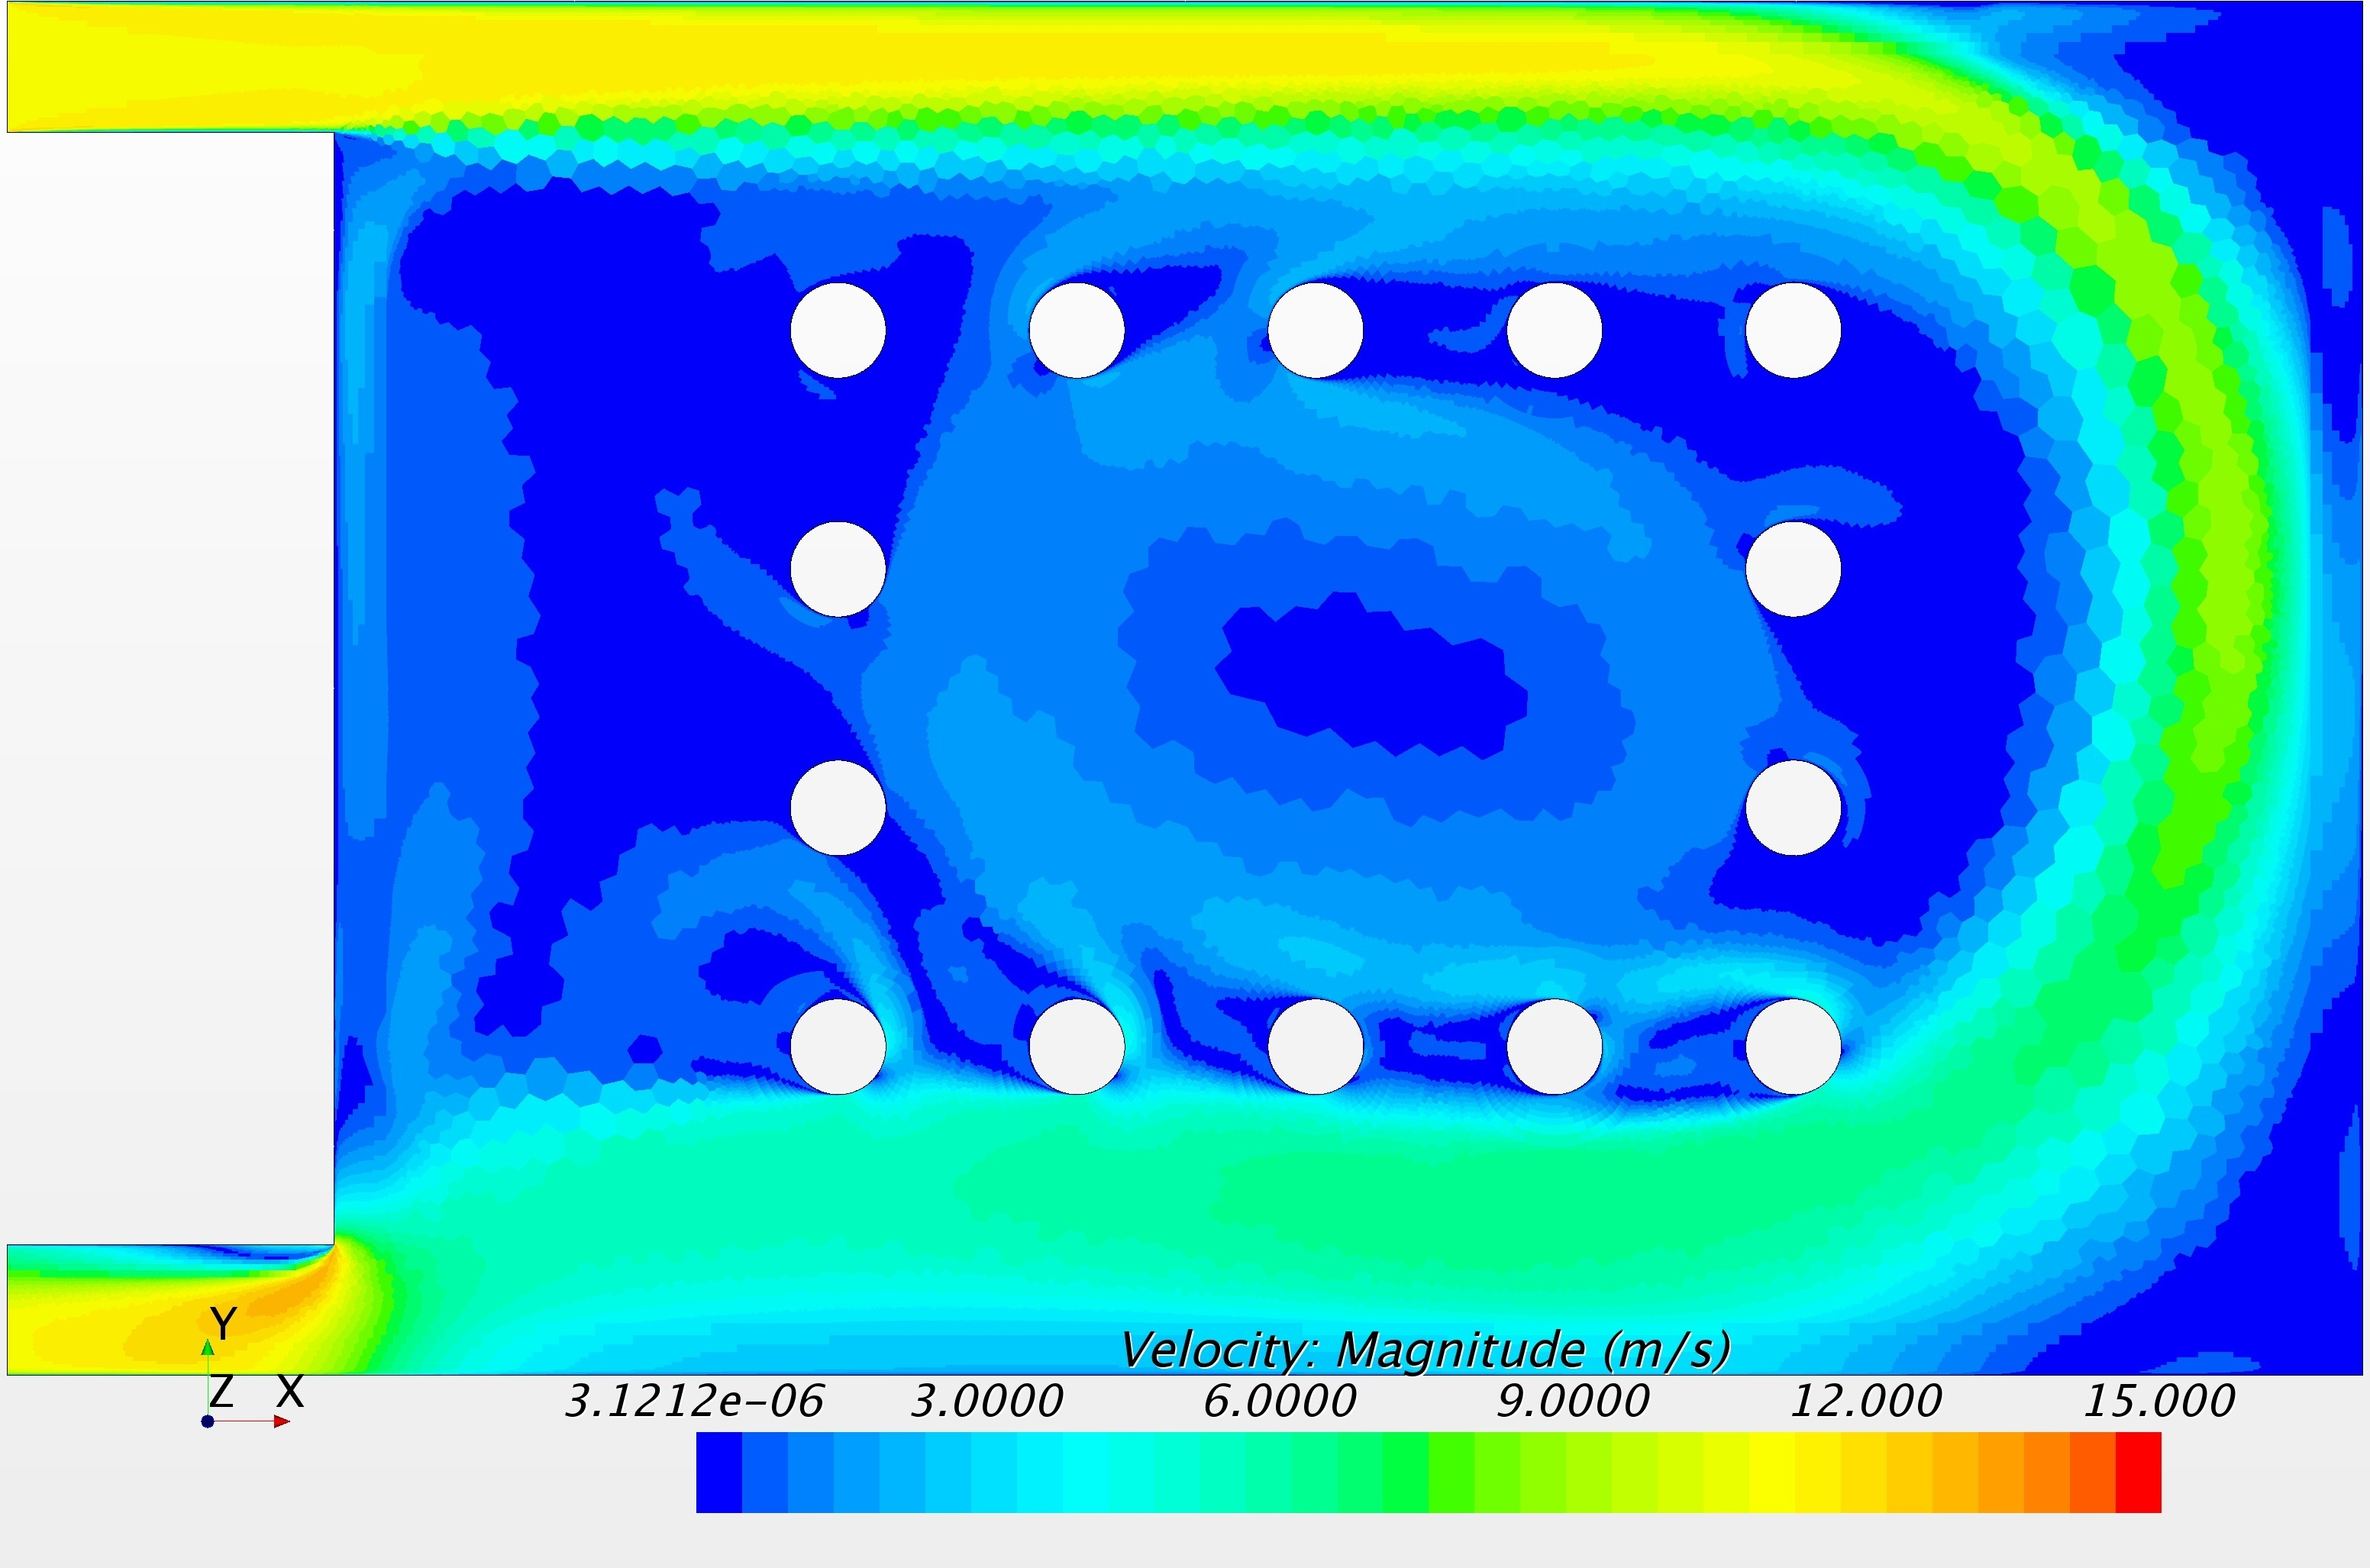
\includegraphics[height=3.8cm]{sources/figure8/c-vel_7.jpg}};
% \node (n8a)  [below=0cm of n7a,anchor=north]  {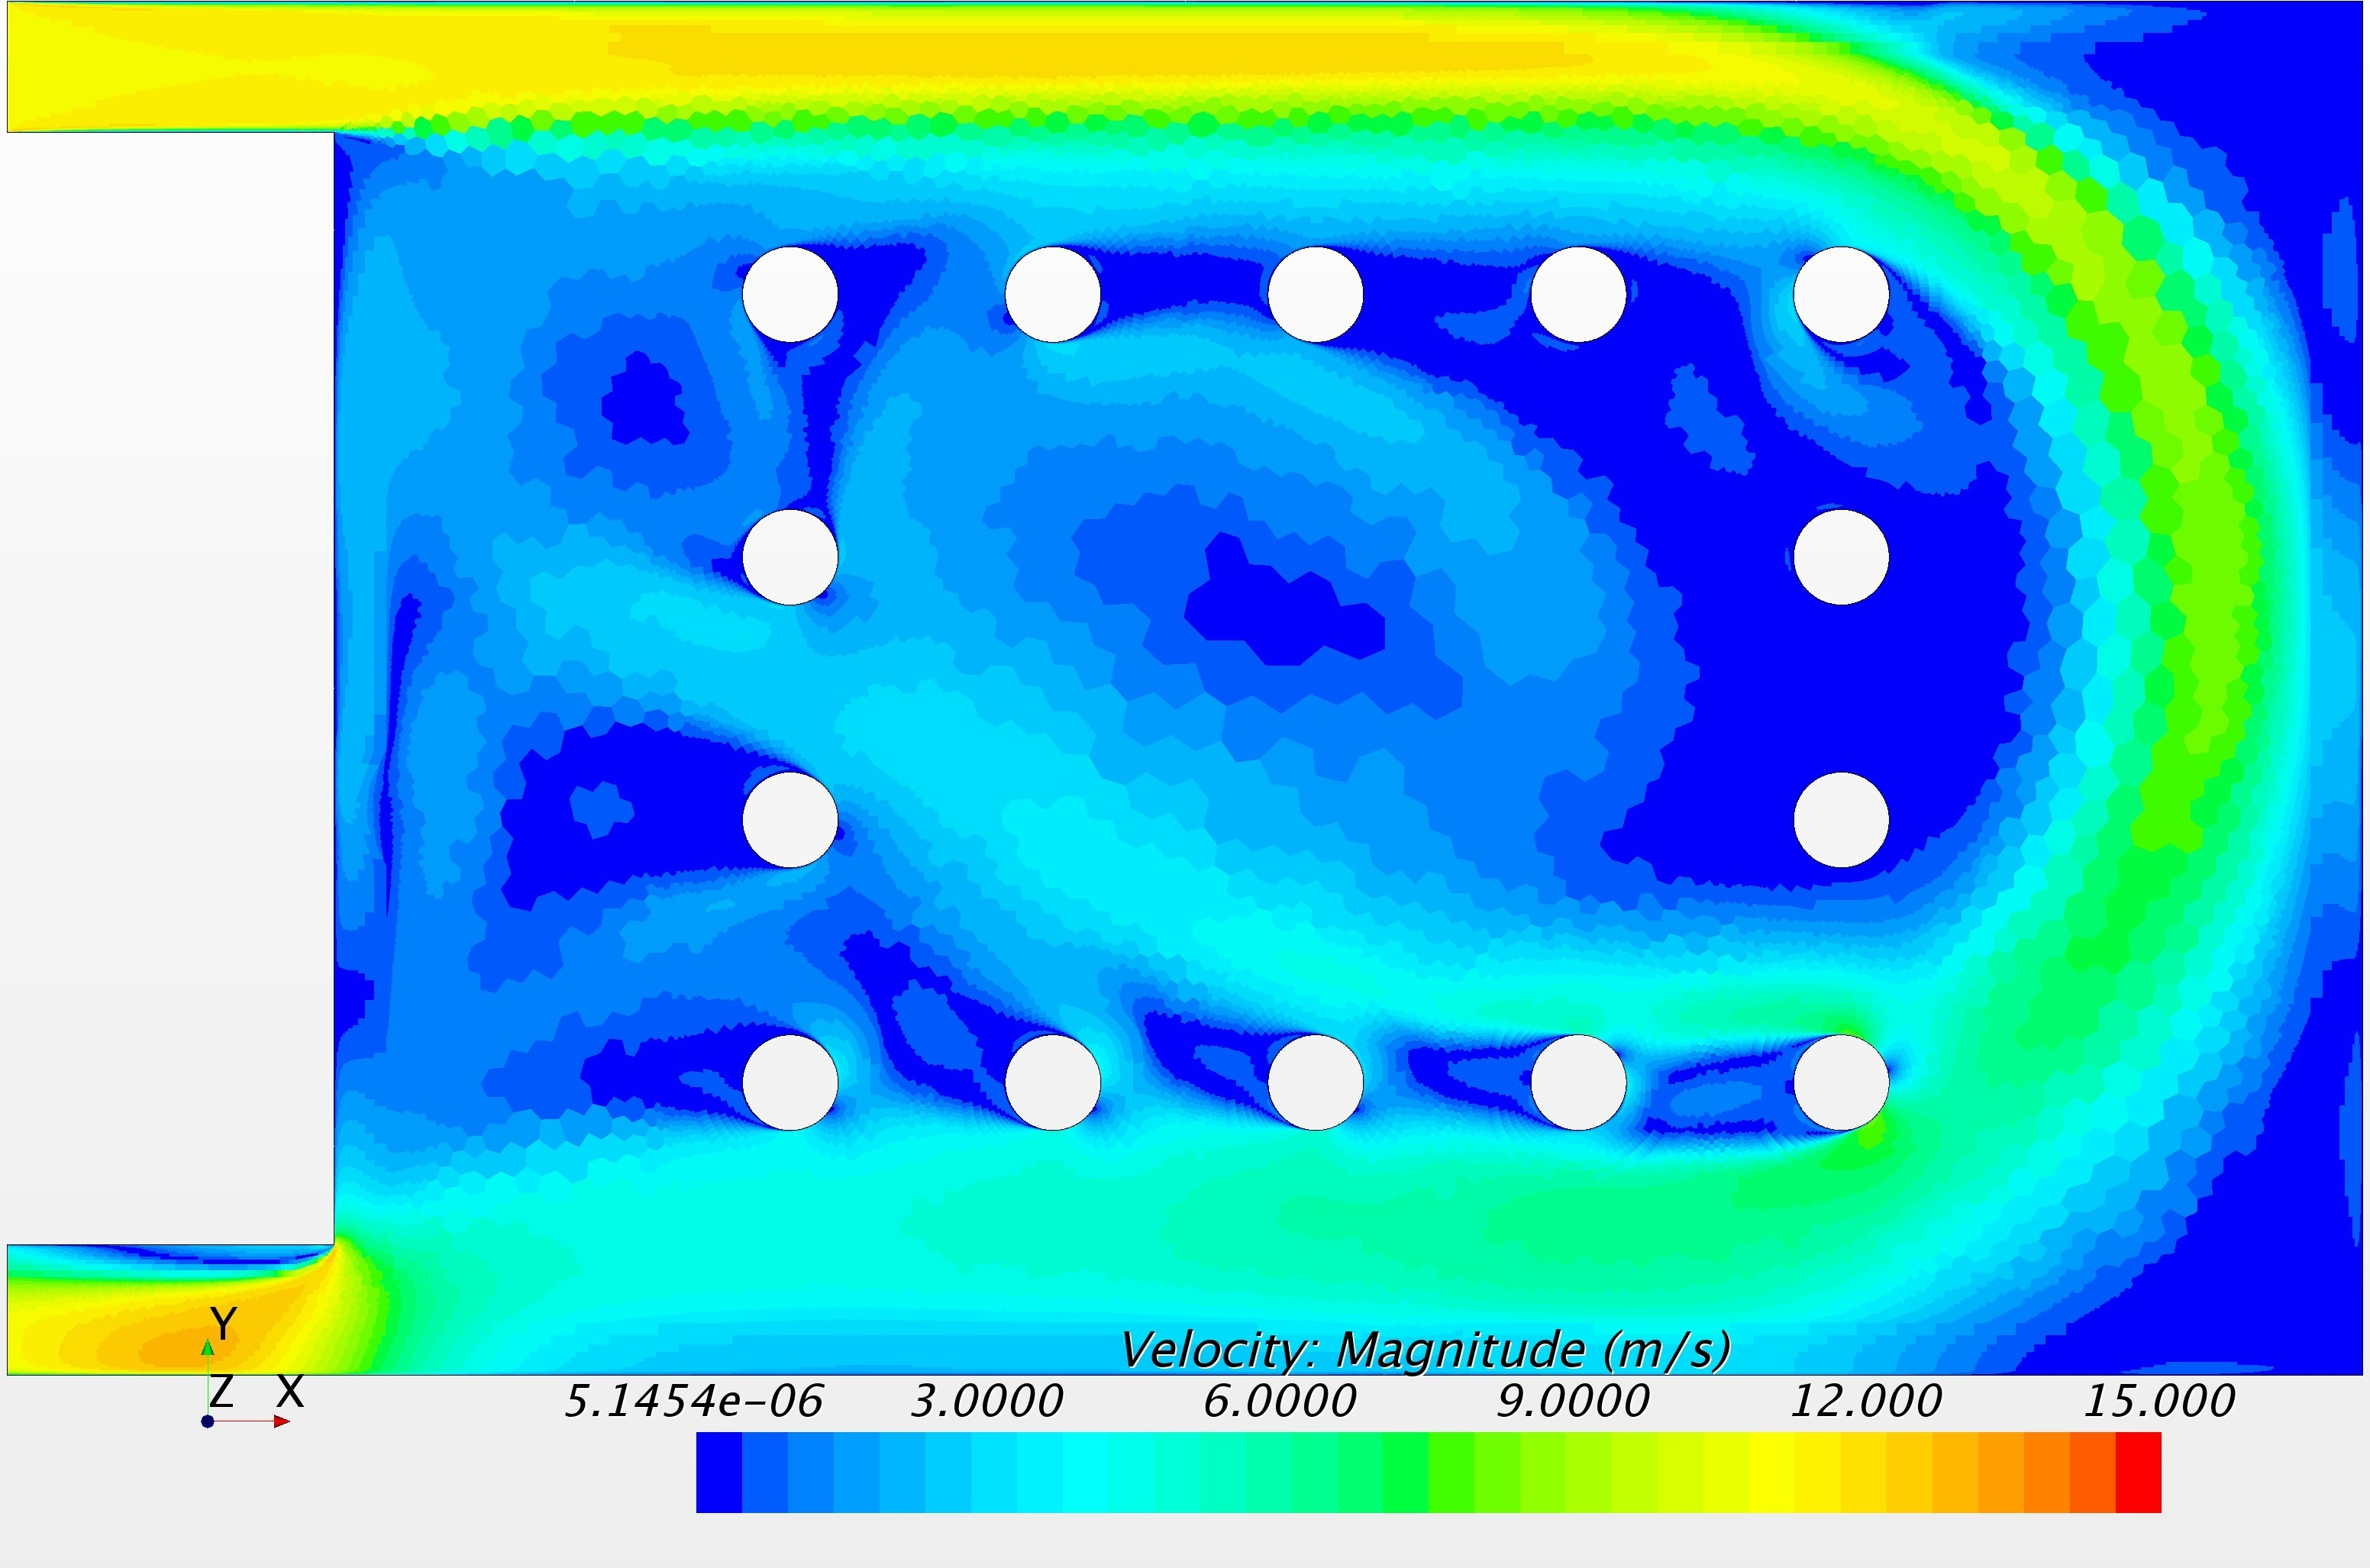
\includegraphics[height=3.8cm]{sources/figure8/c-vel_8.jpg}};
% \node (n9a)  [below=0cm of n8a,anchor=north]  {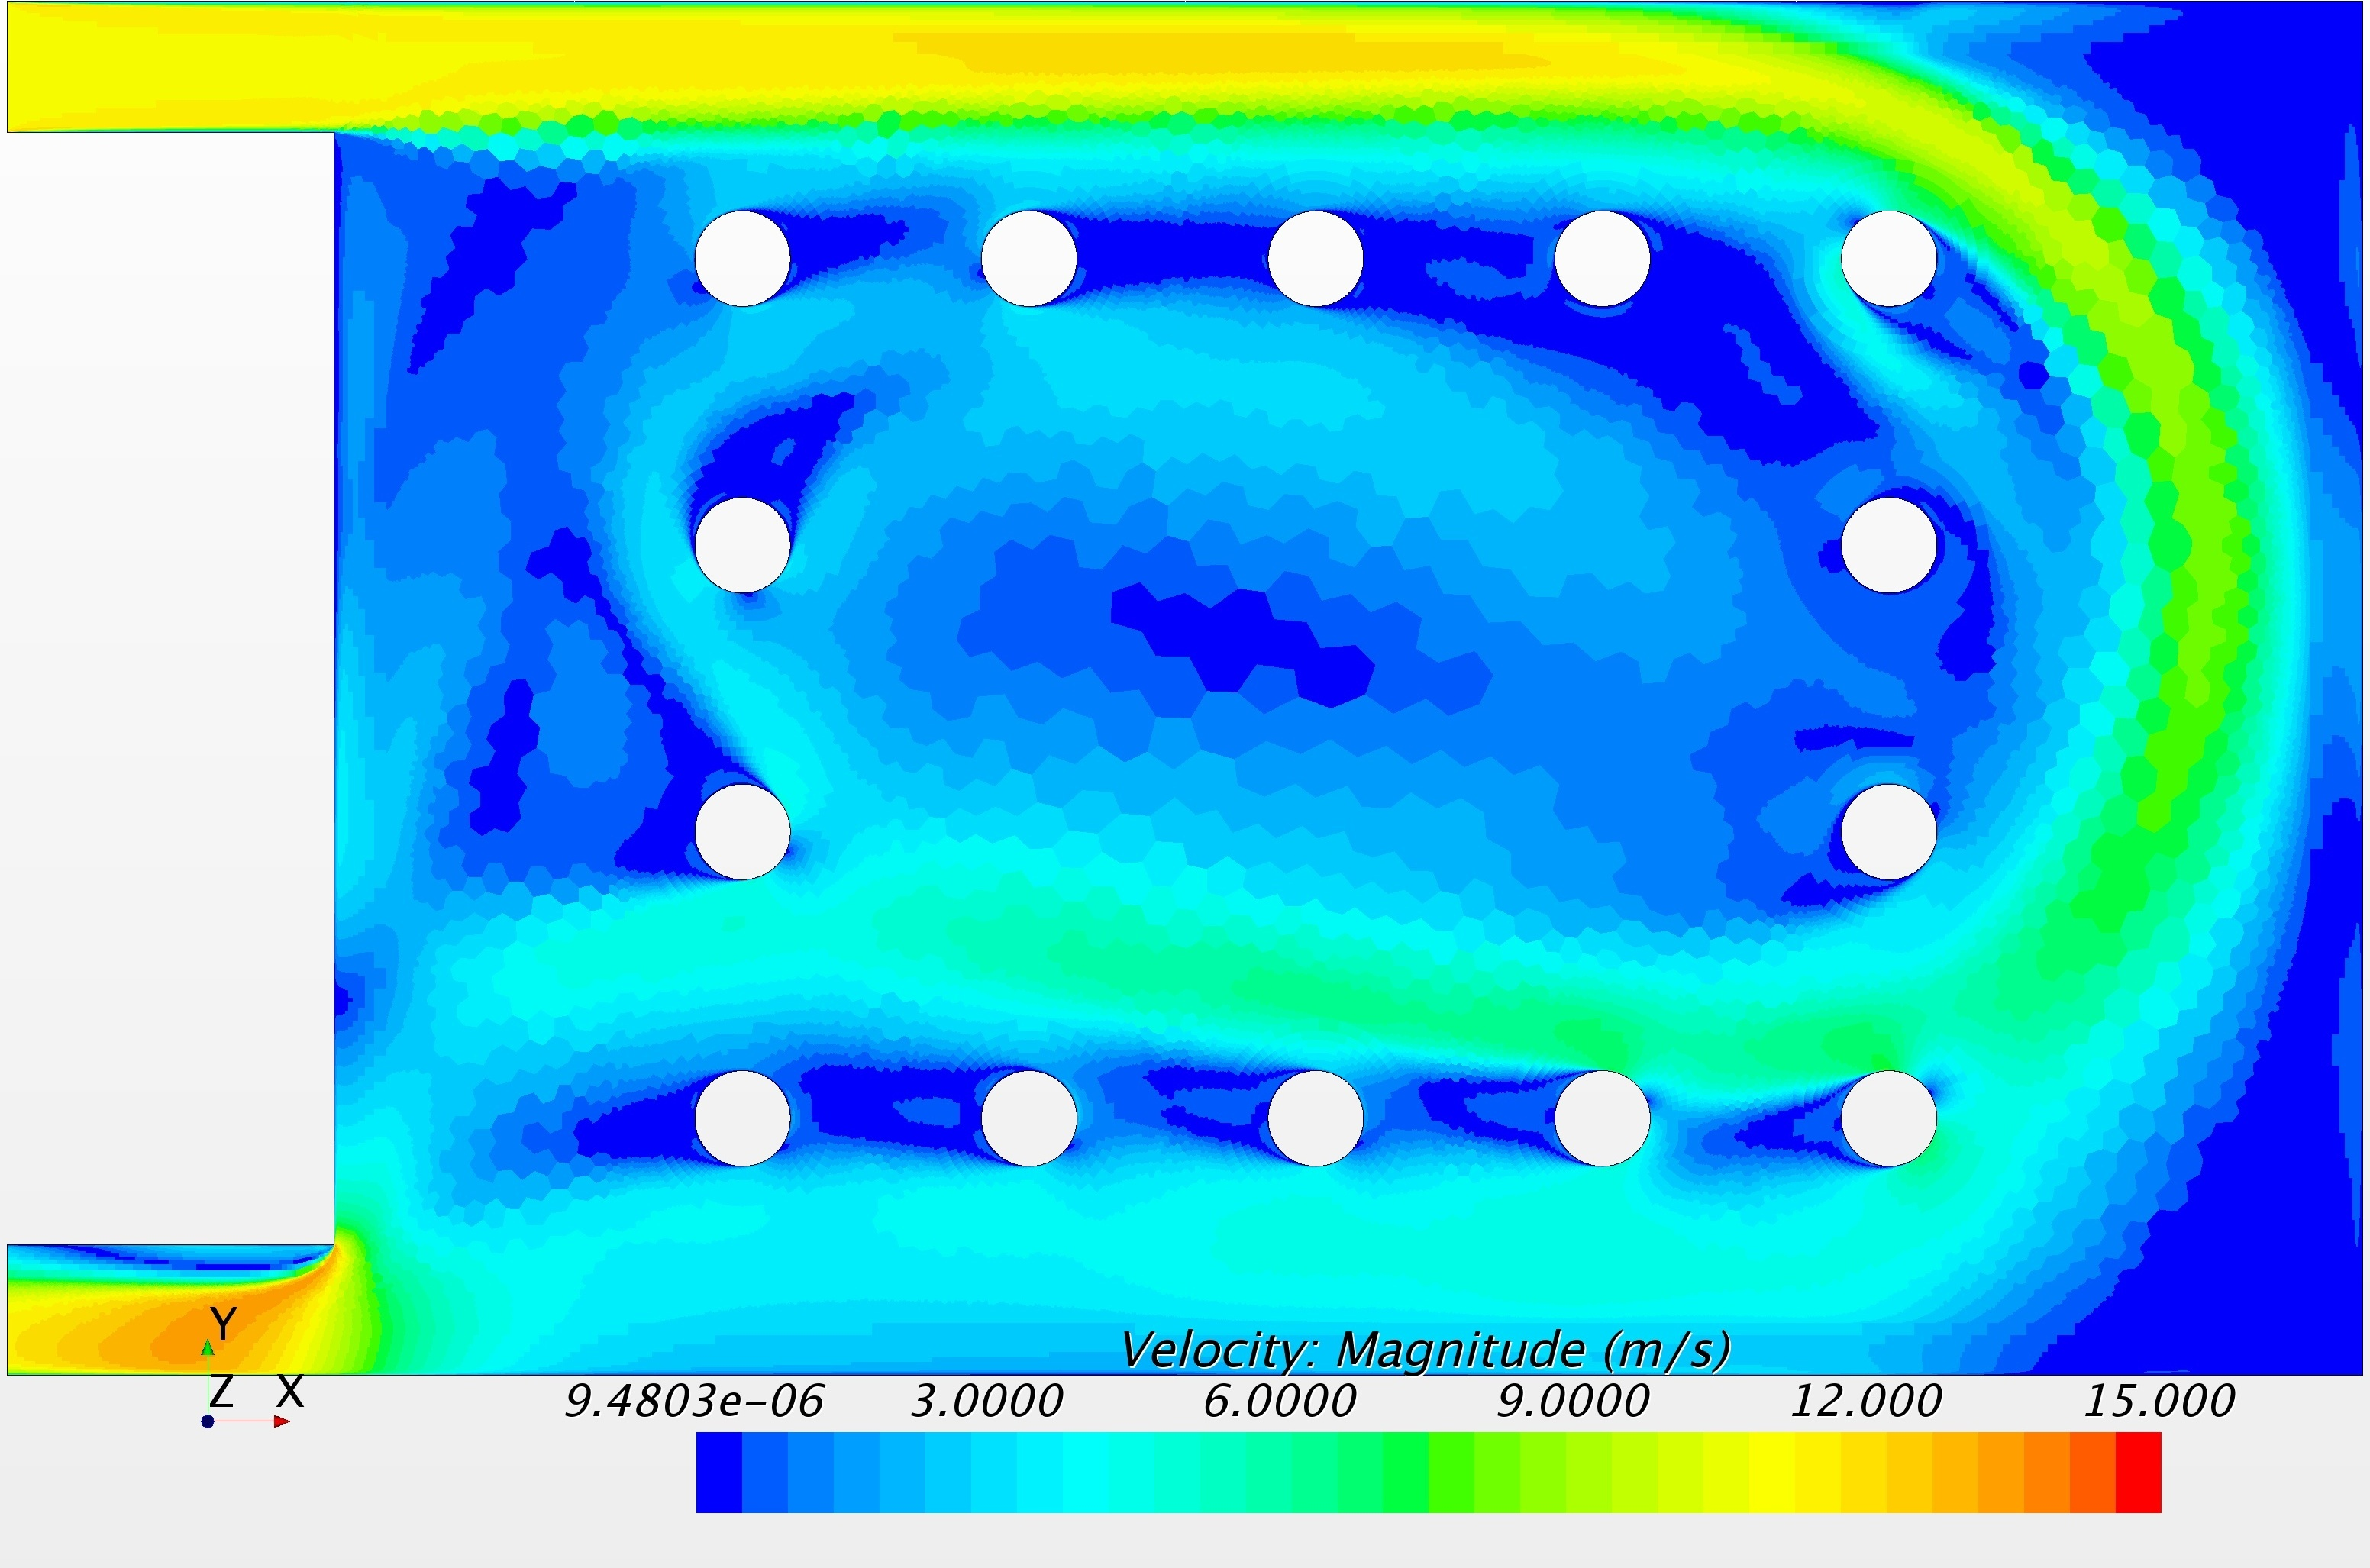
\includegraphics[height=3.8cm]{sources/figure8/c-vel_9.jpg}};
\node (n10a) [below=0cm of n7a,anchor=north]  {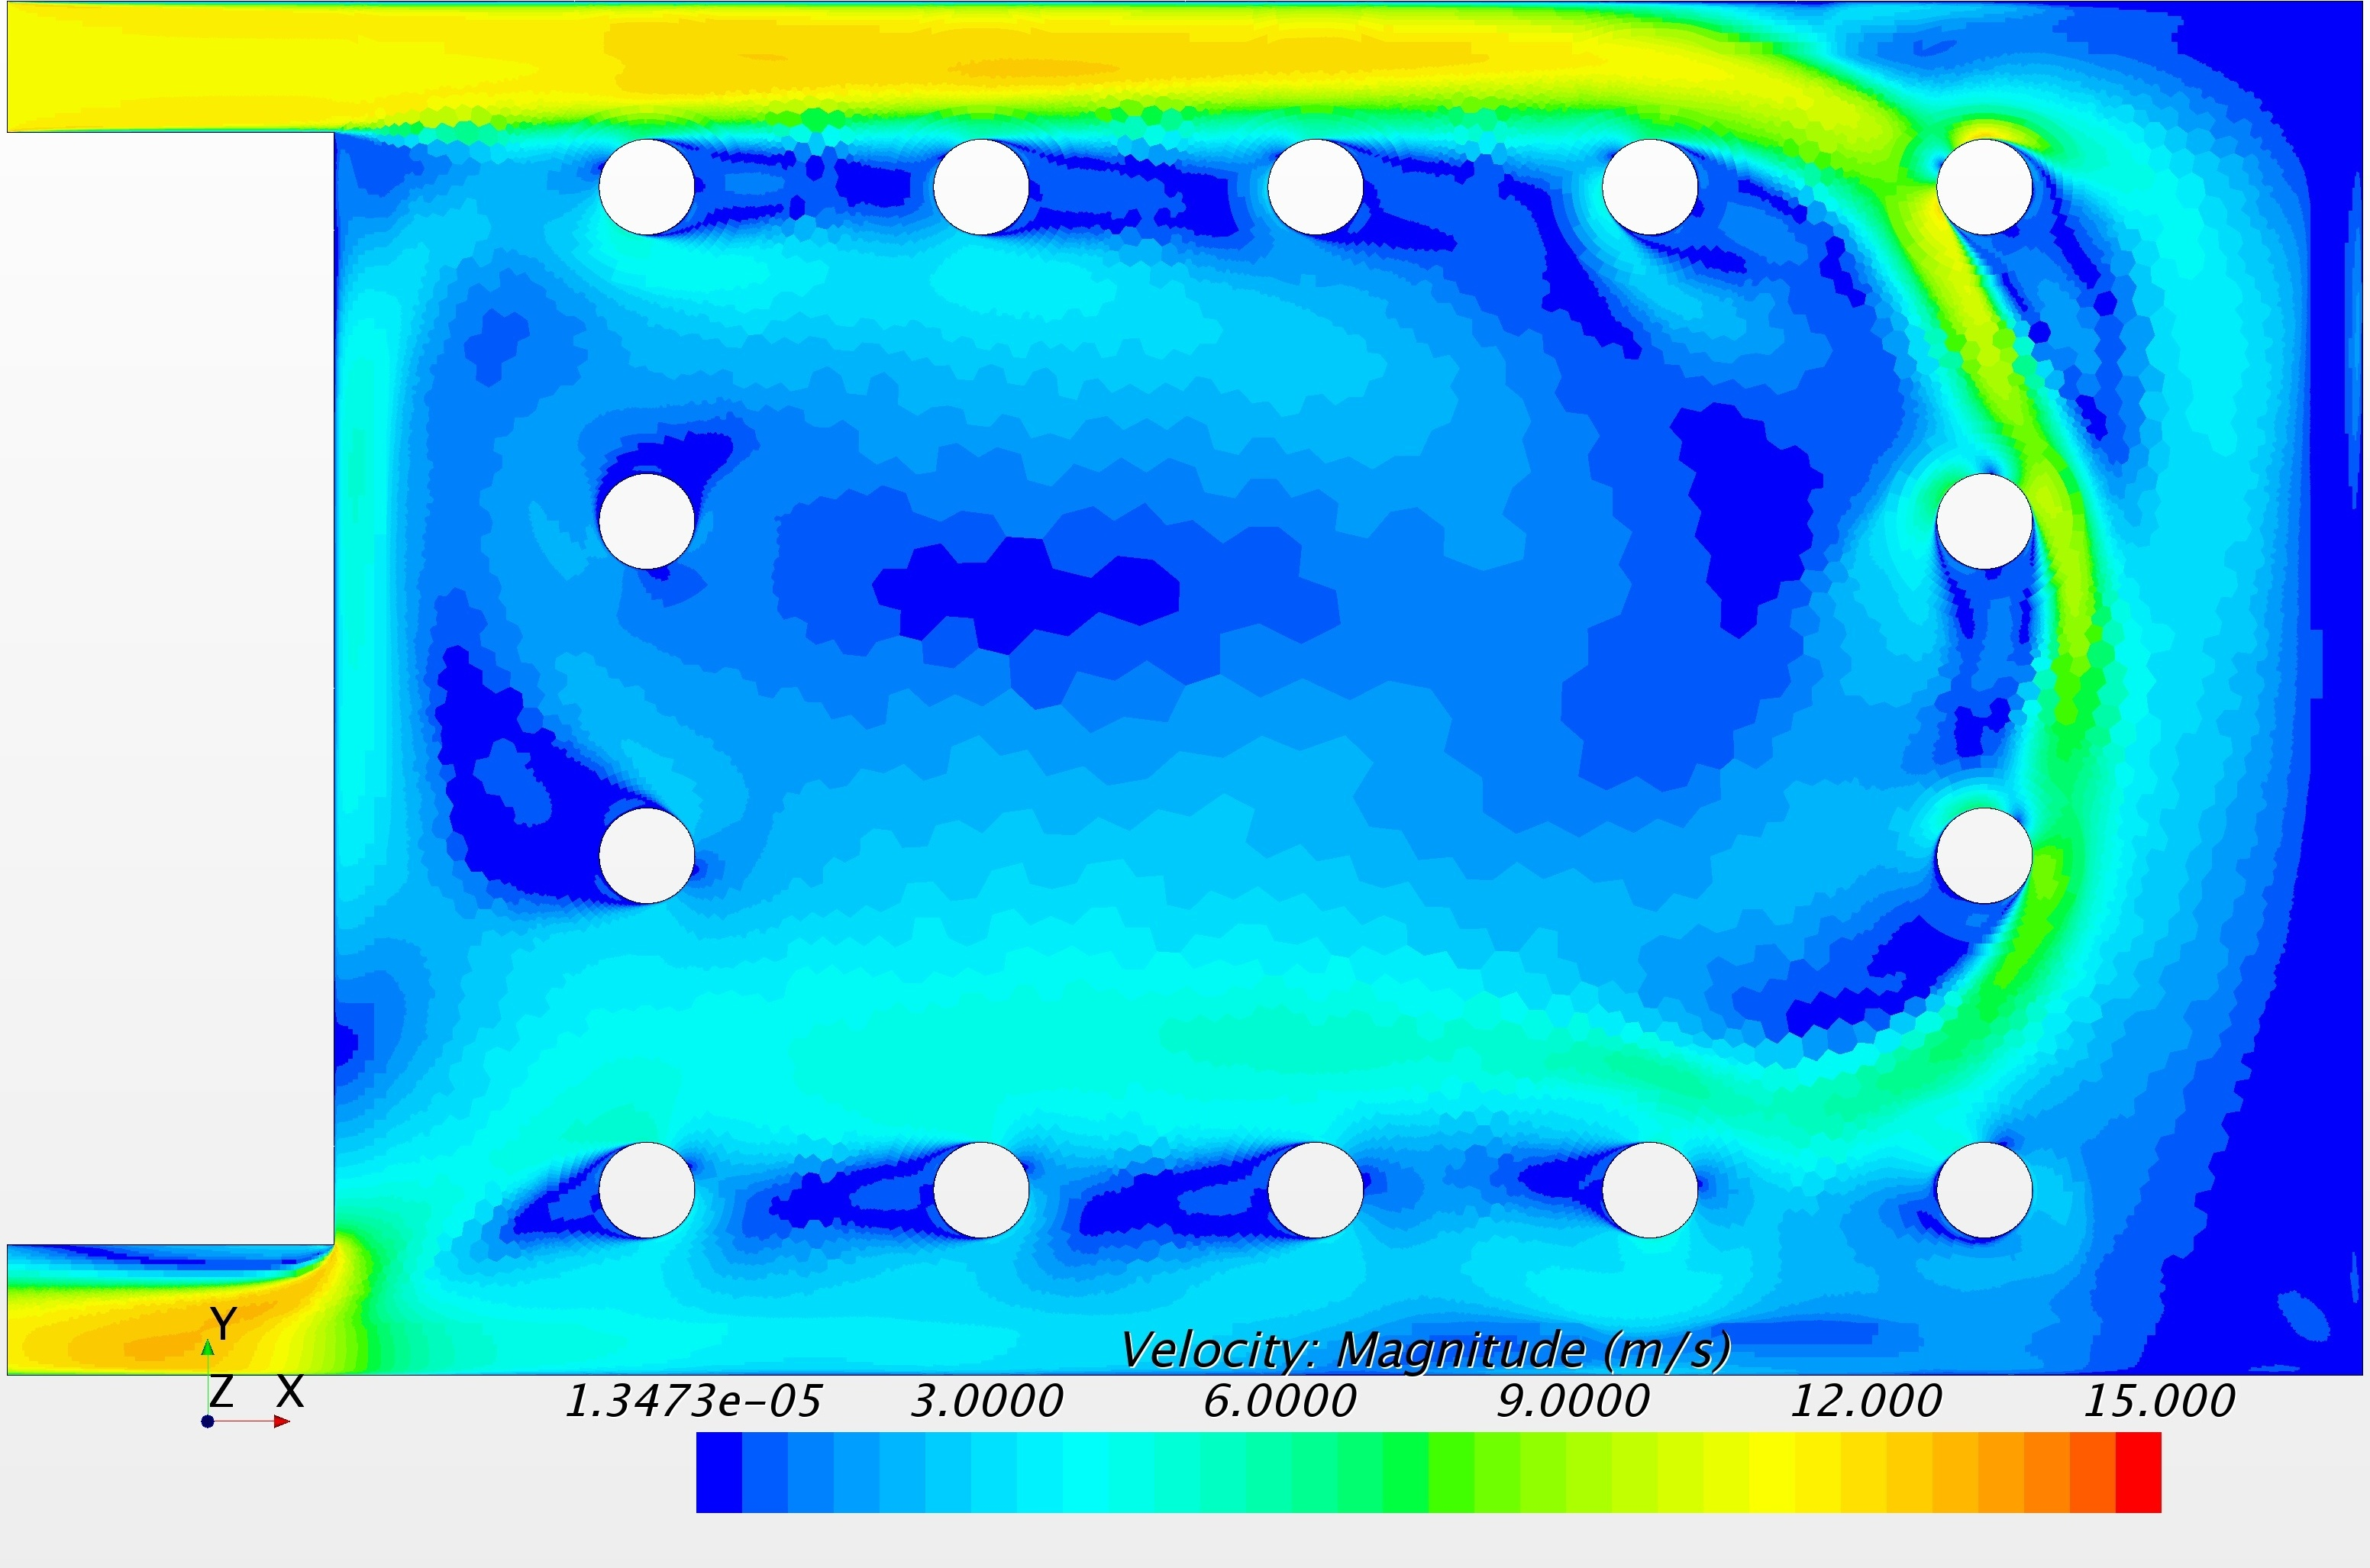
\includegraphics[height=3.8cm]{sources/figure8/c-vel_10.jpg}};
\node (n11a) [below=0cm of n10a,anchor=north] {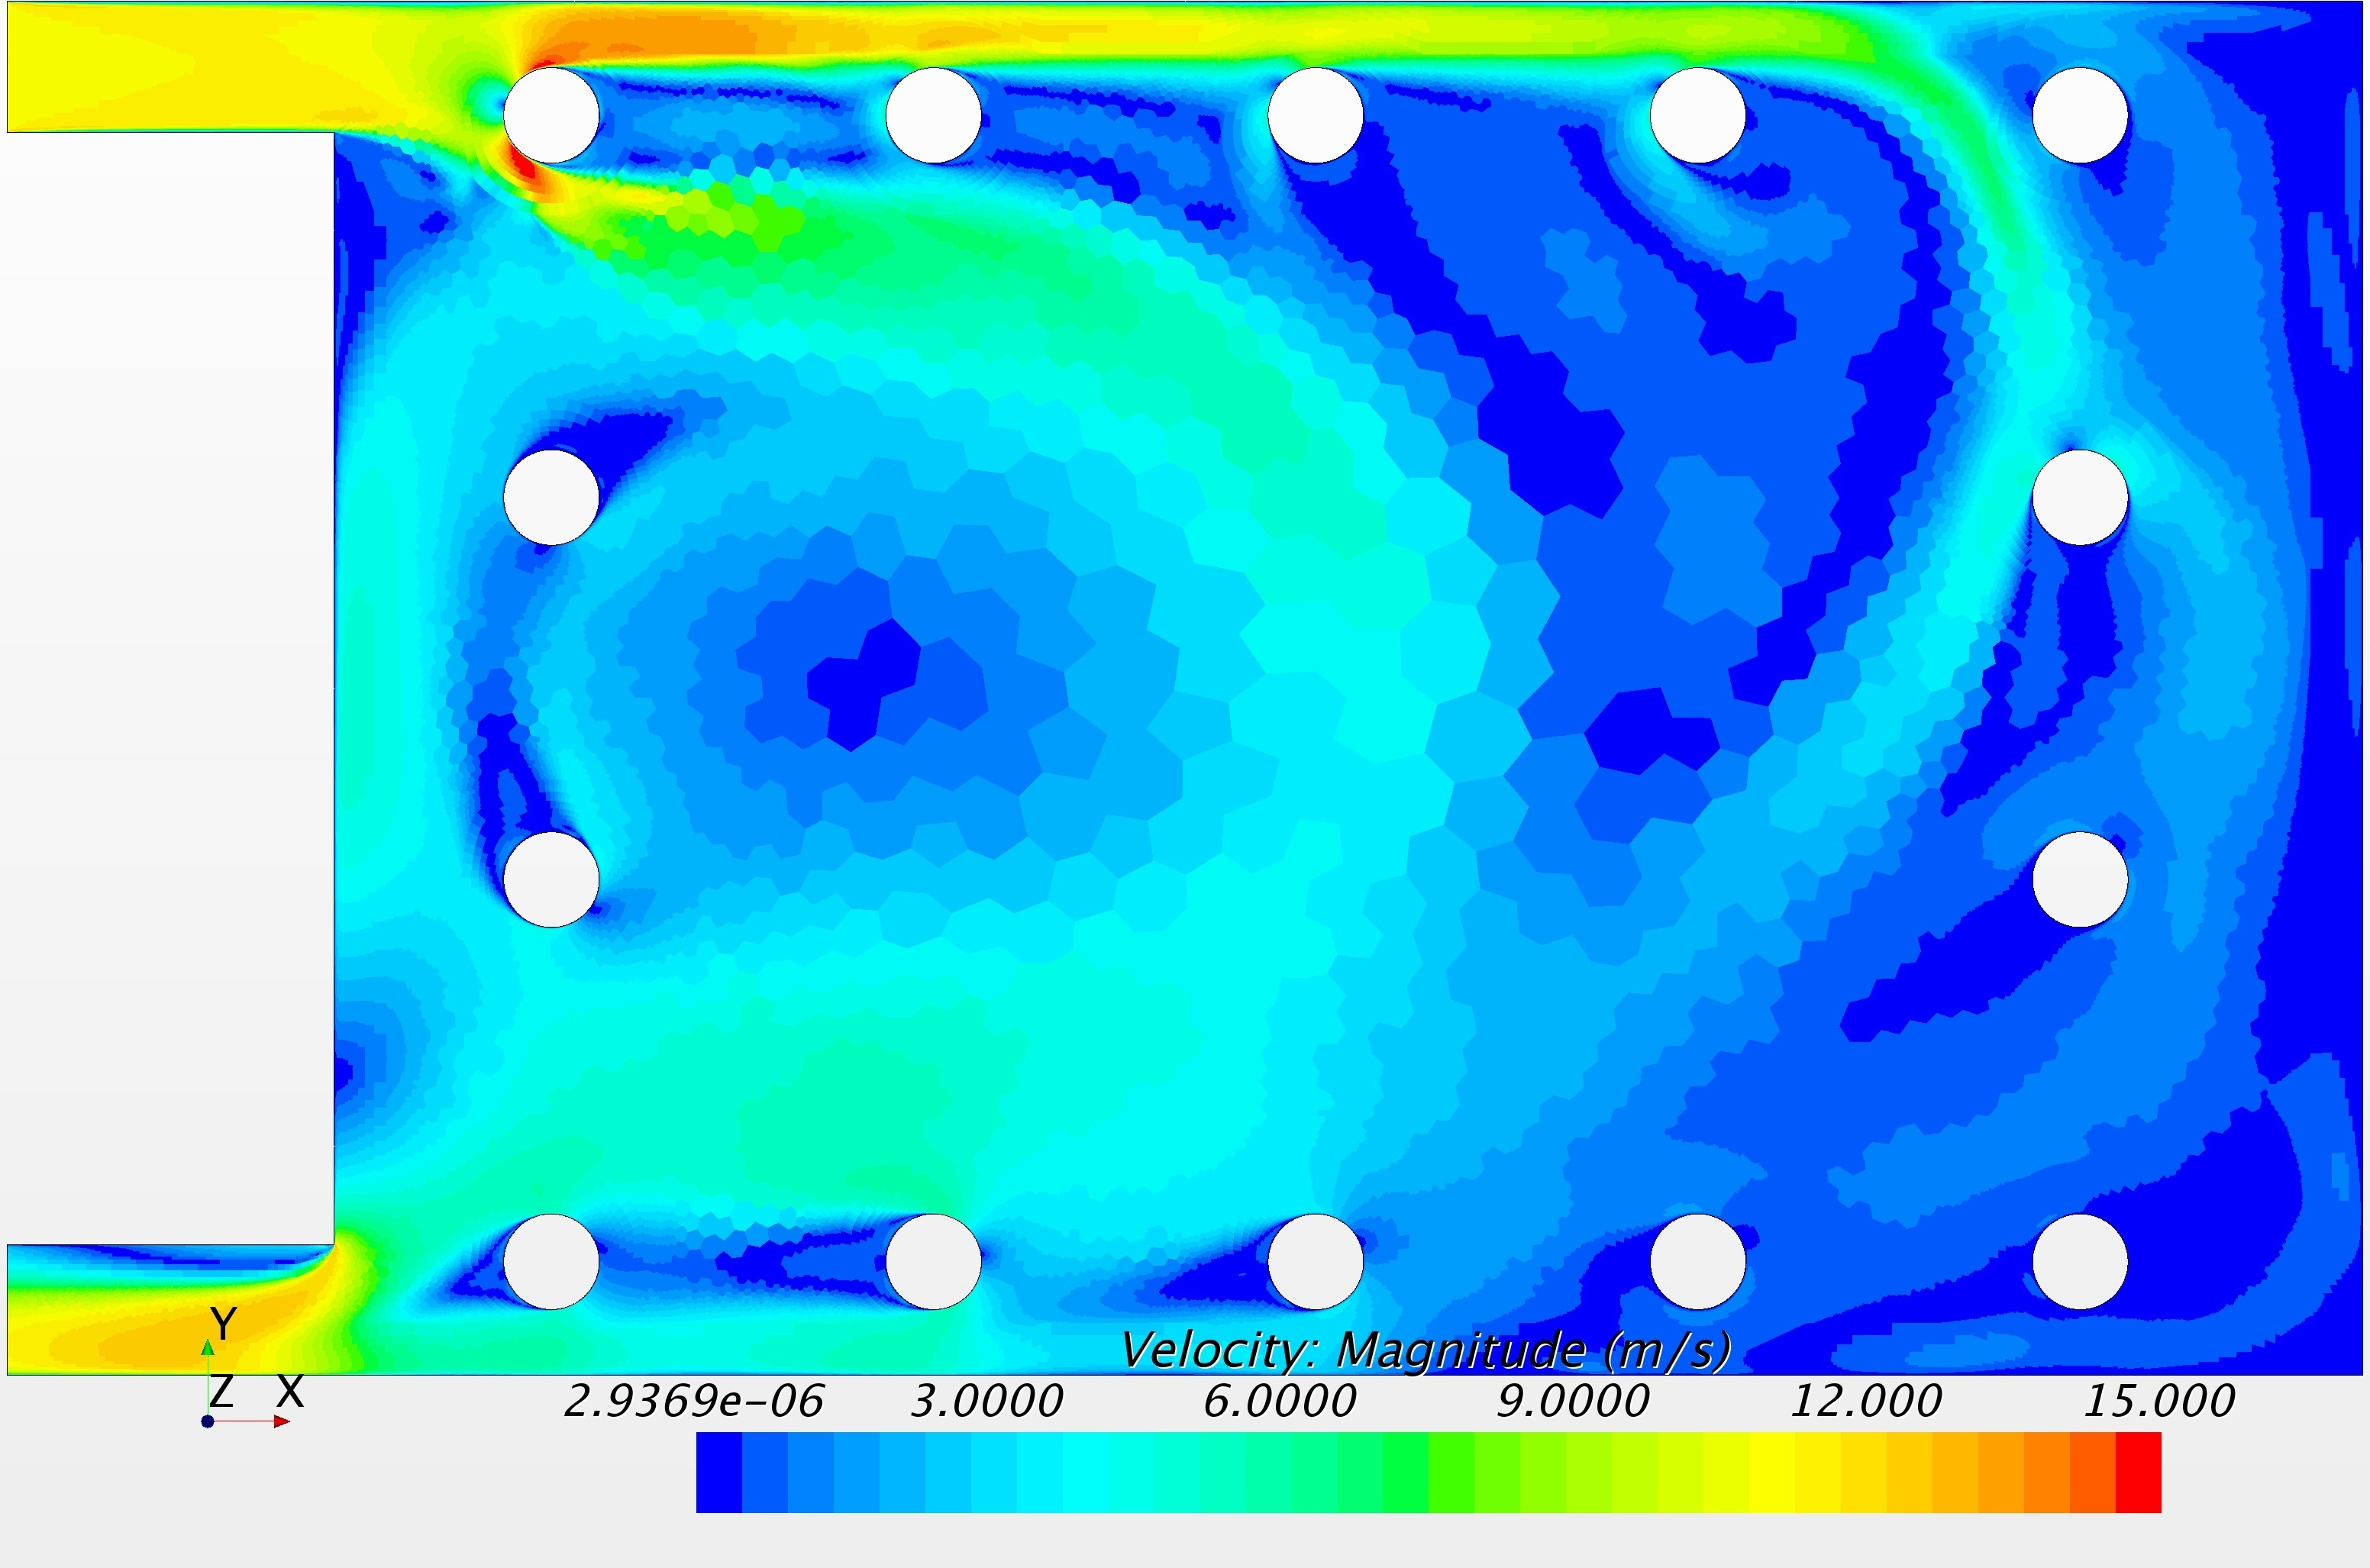
\includegraphics[height=3.8cm]{sources/figure8/c-vel_11.jpg}};
% \node (n12a) [below=0cm of n11a,anchor=north] {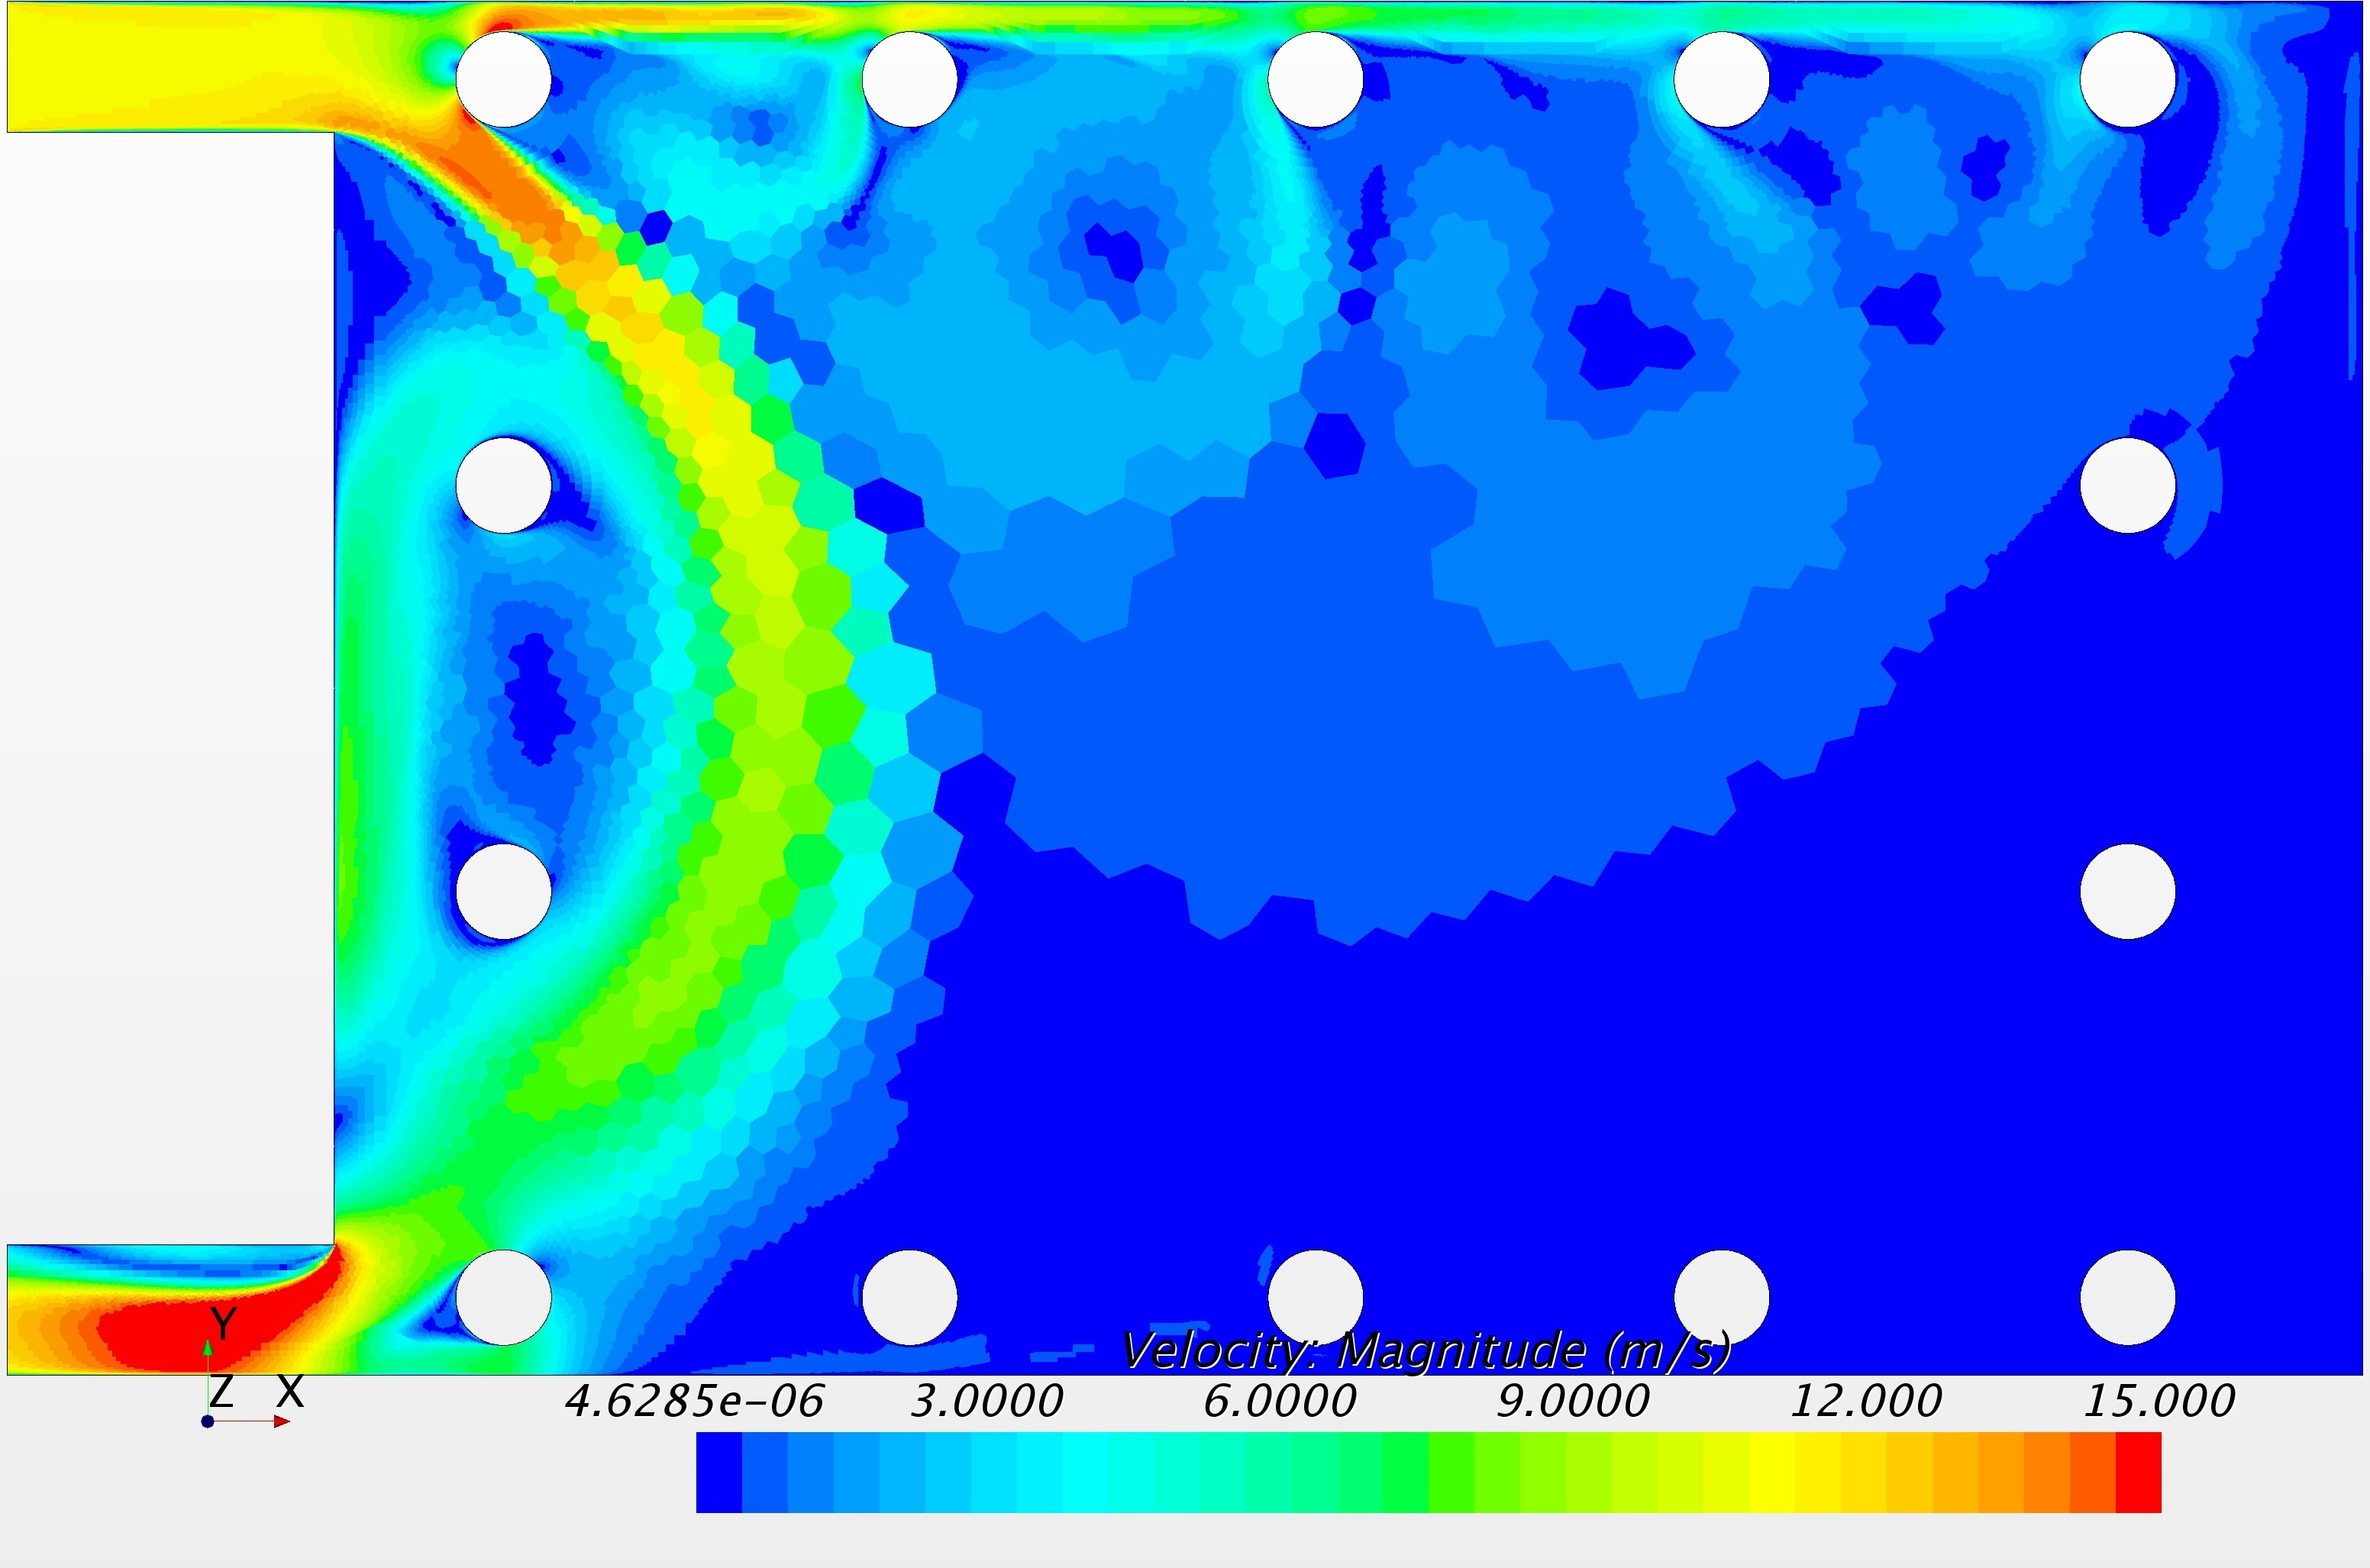
\includegraphics[height=3.8cm]{sources/figure8/c-vel_12.jpg}};


\node (n1b)  [right=0.05cm of n1a]   {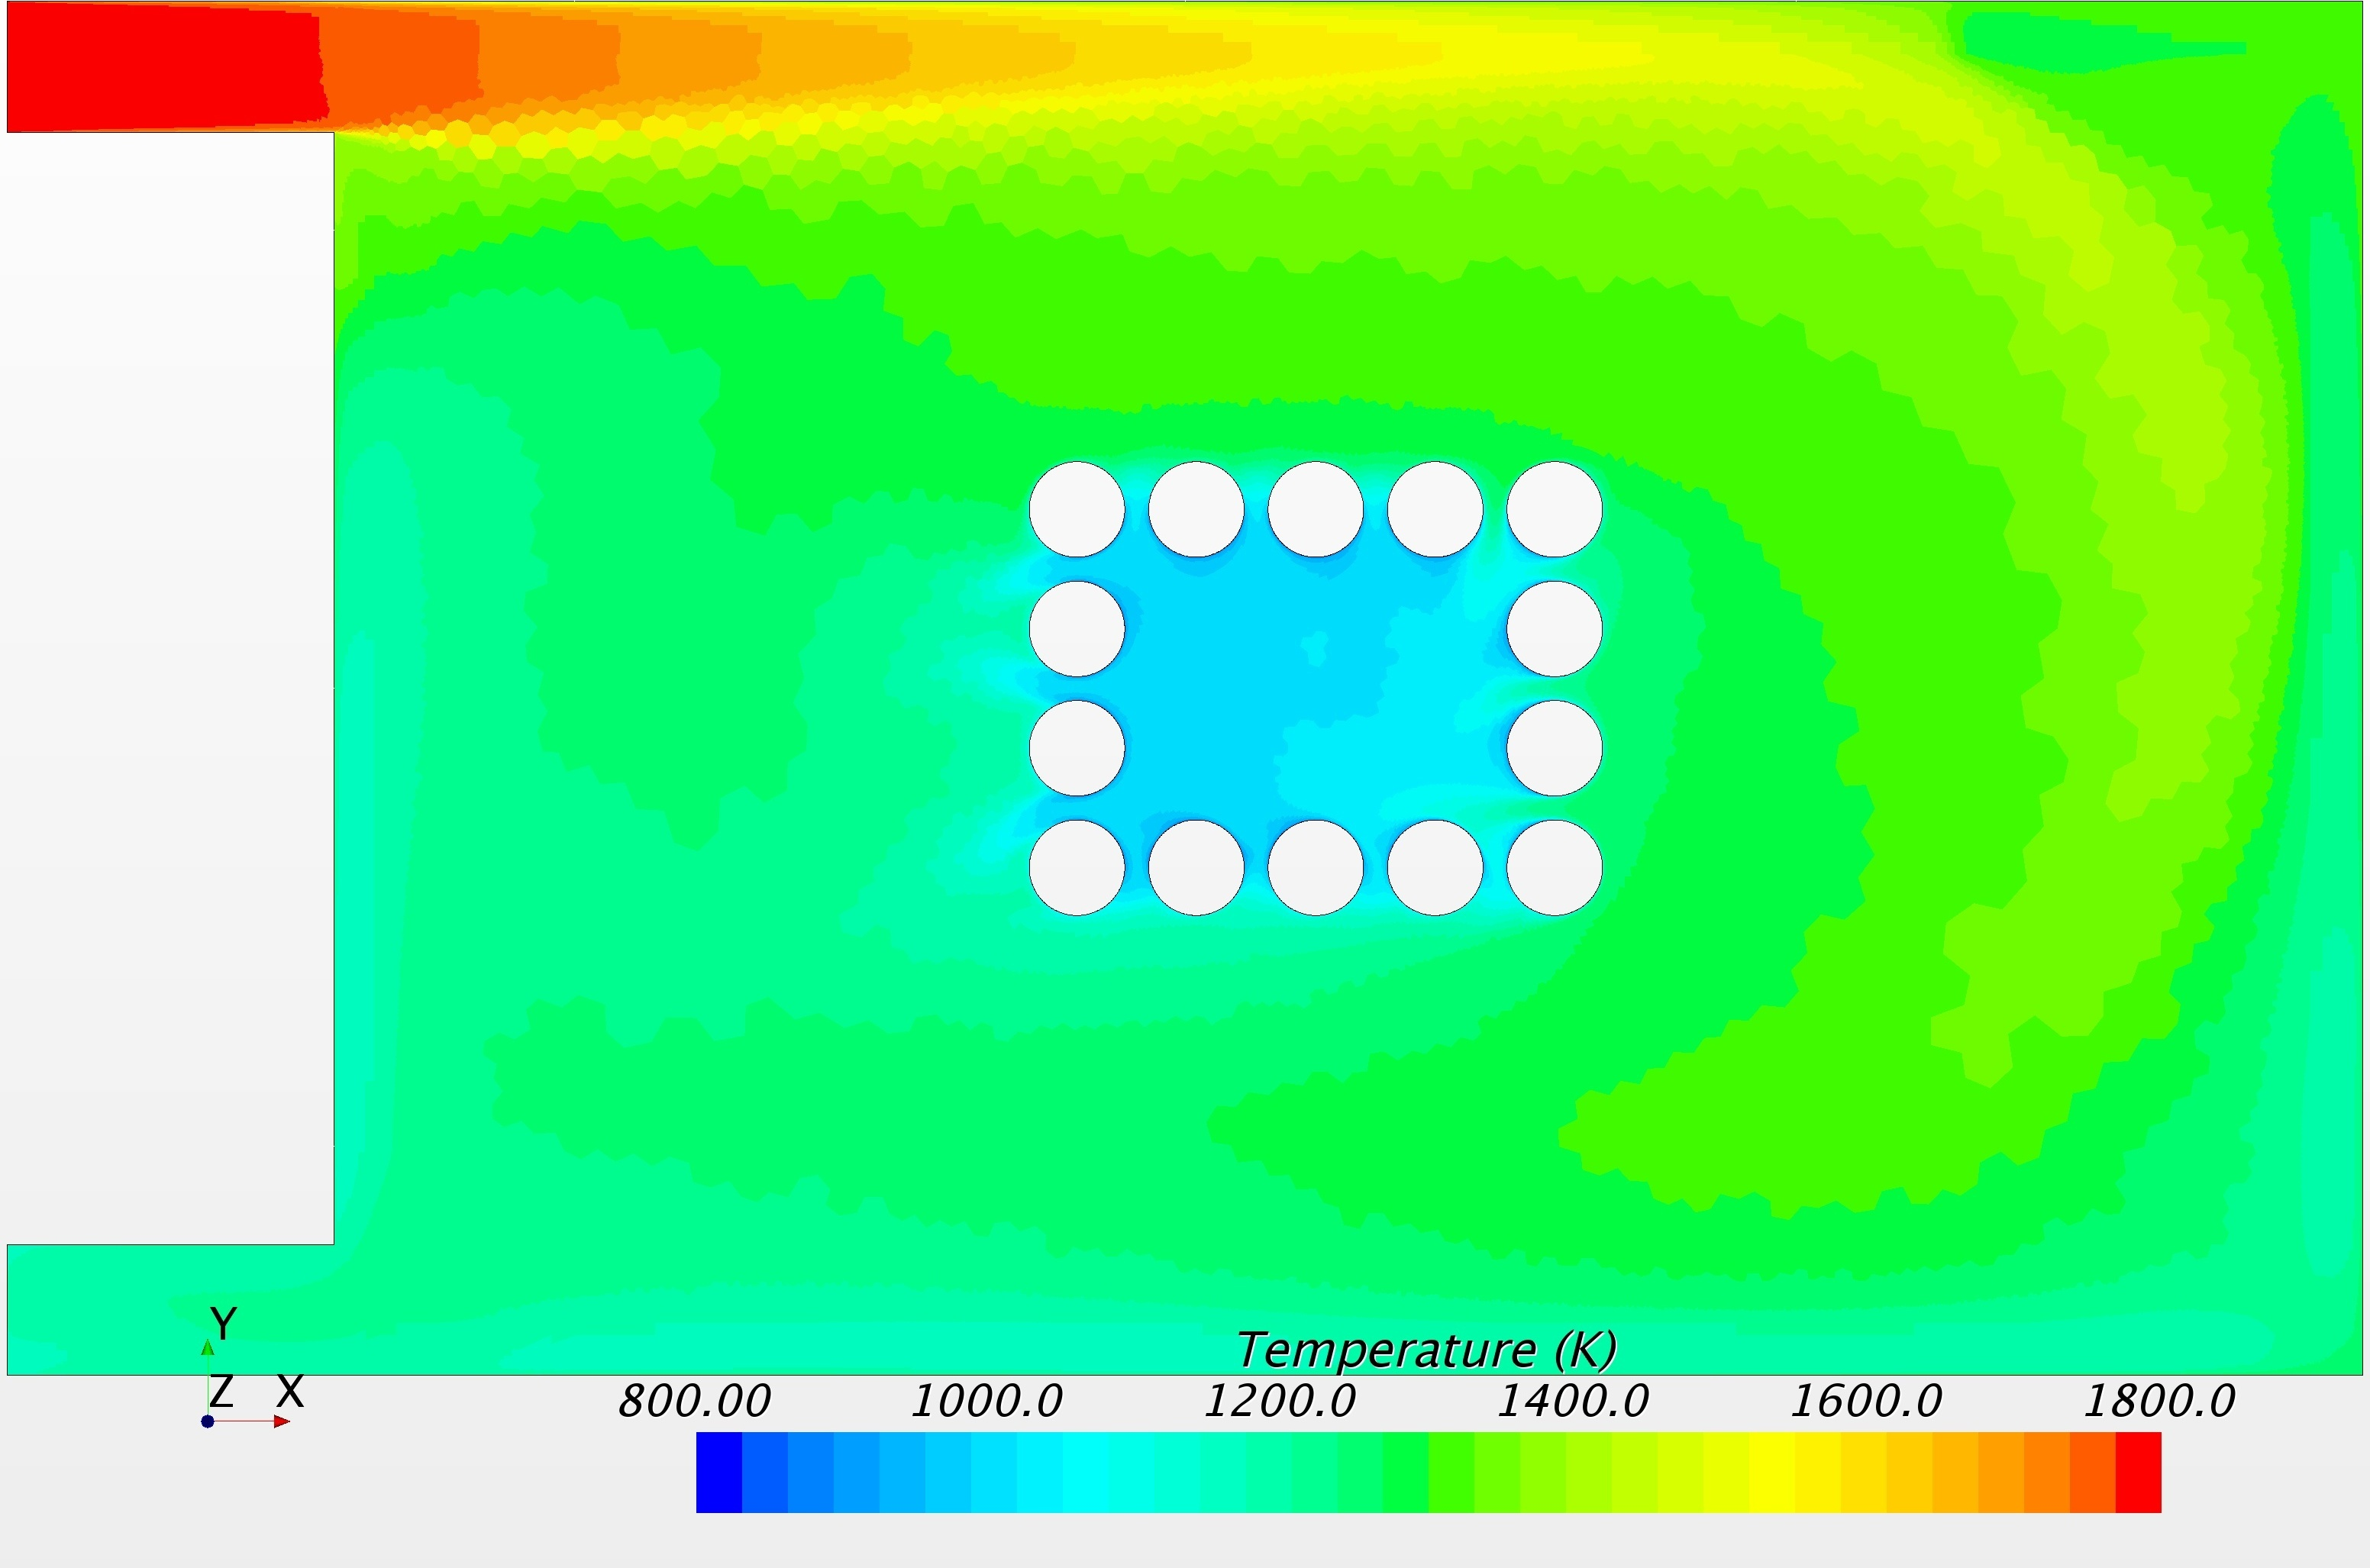
\includegraphics[height=3.8cm]{sources/figure8/c-temp_1.jpg}};
% \node (n2b)  [right=0.05cm of n2a]   {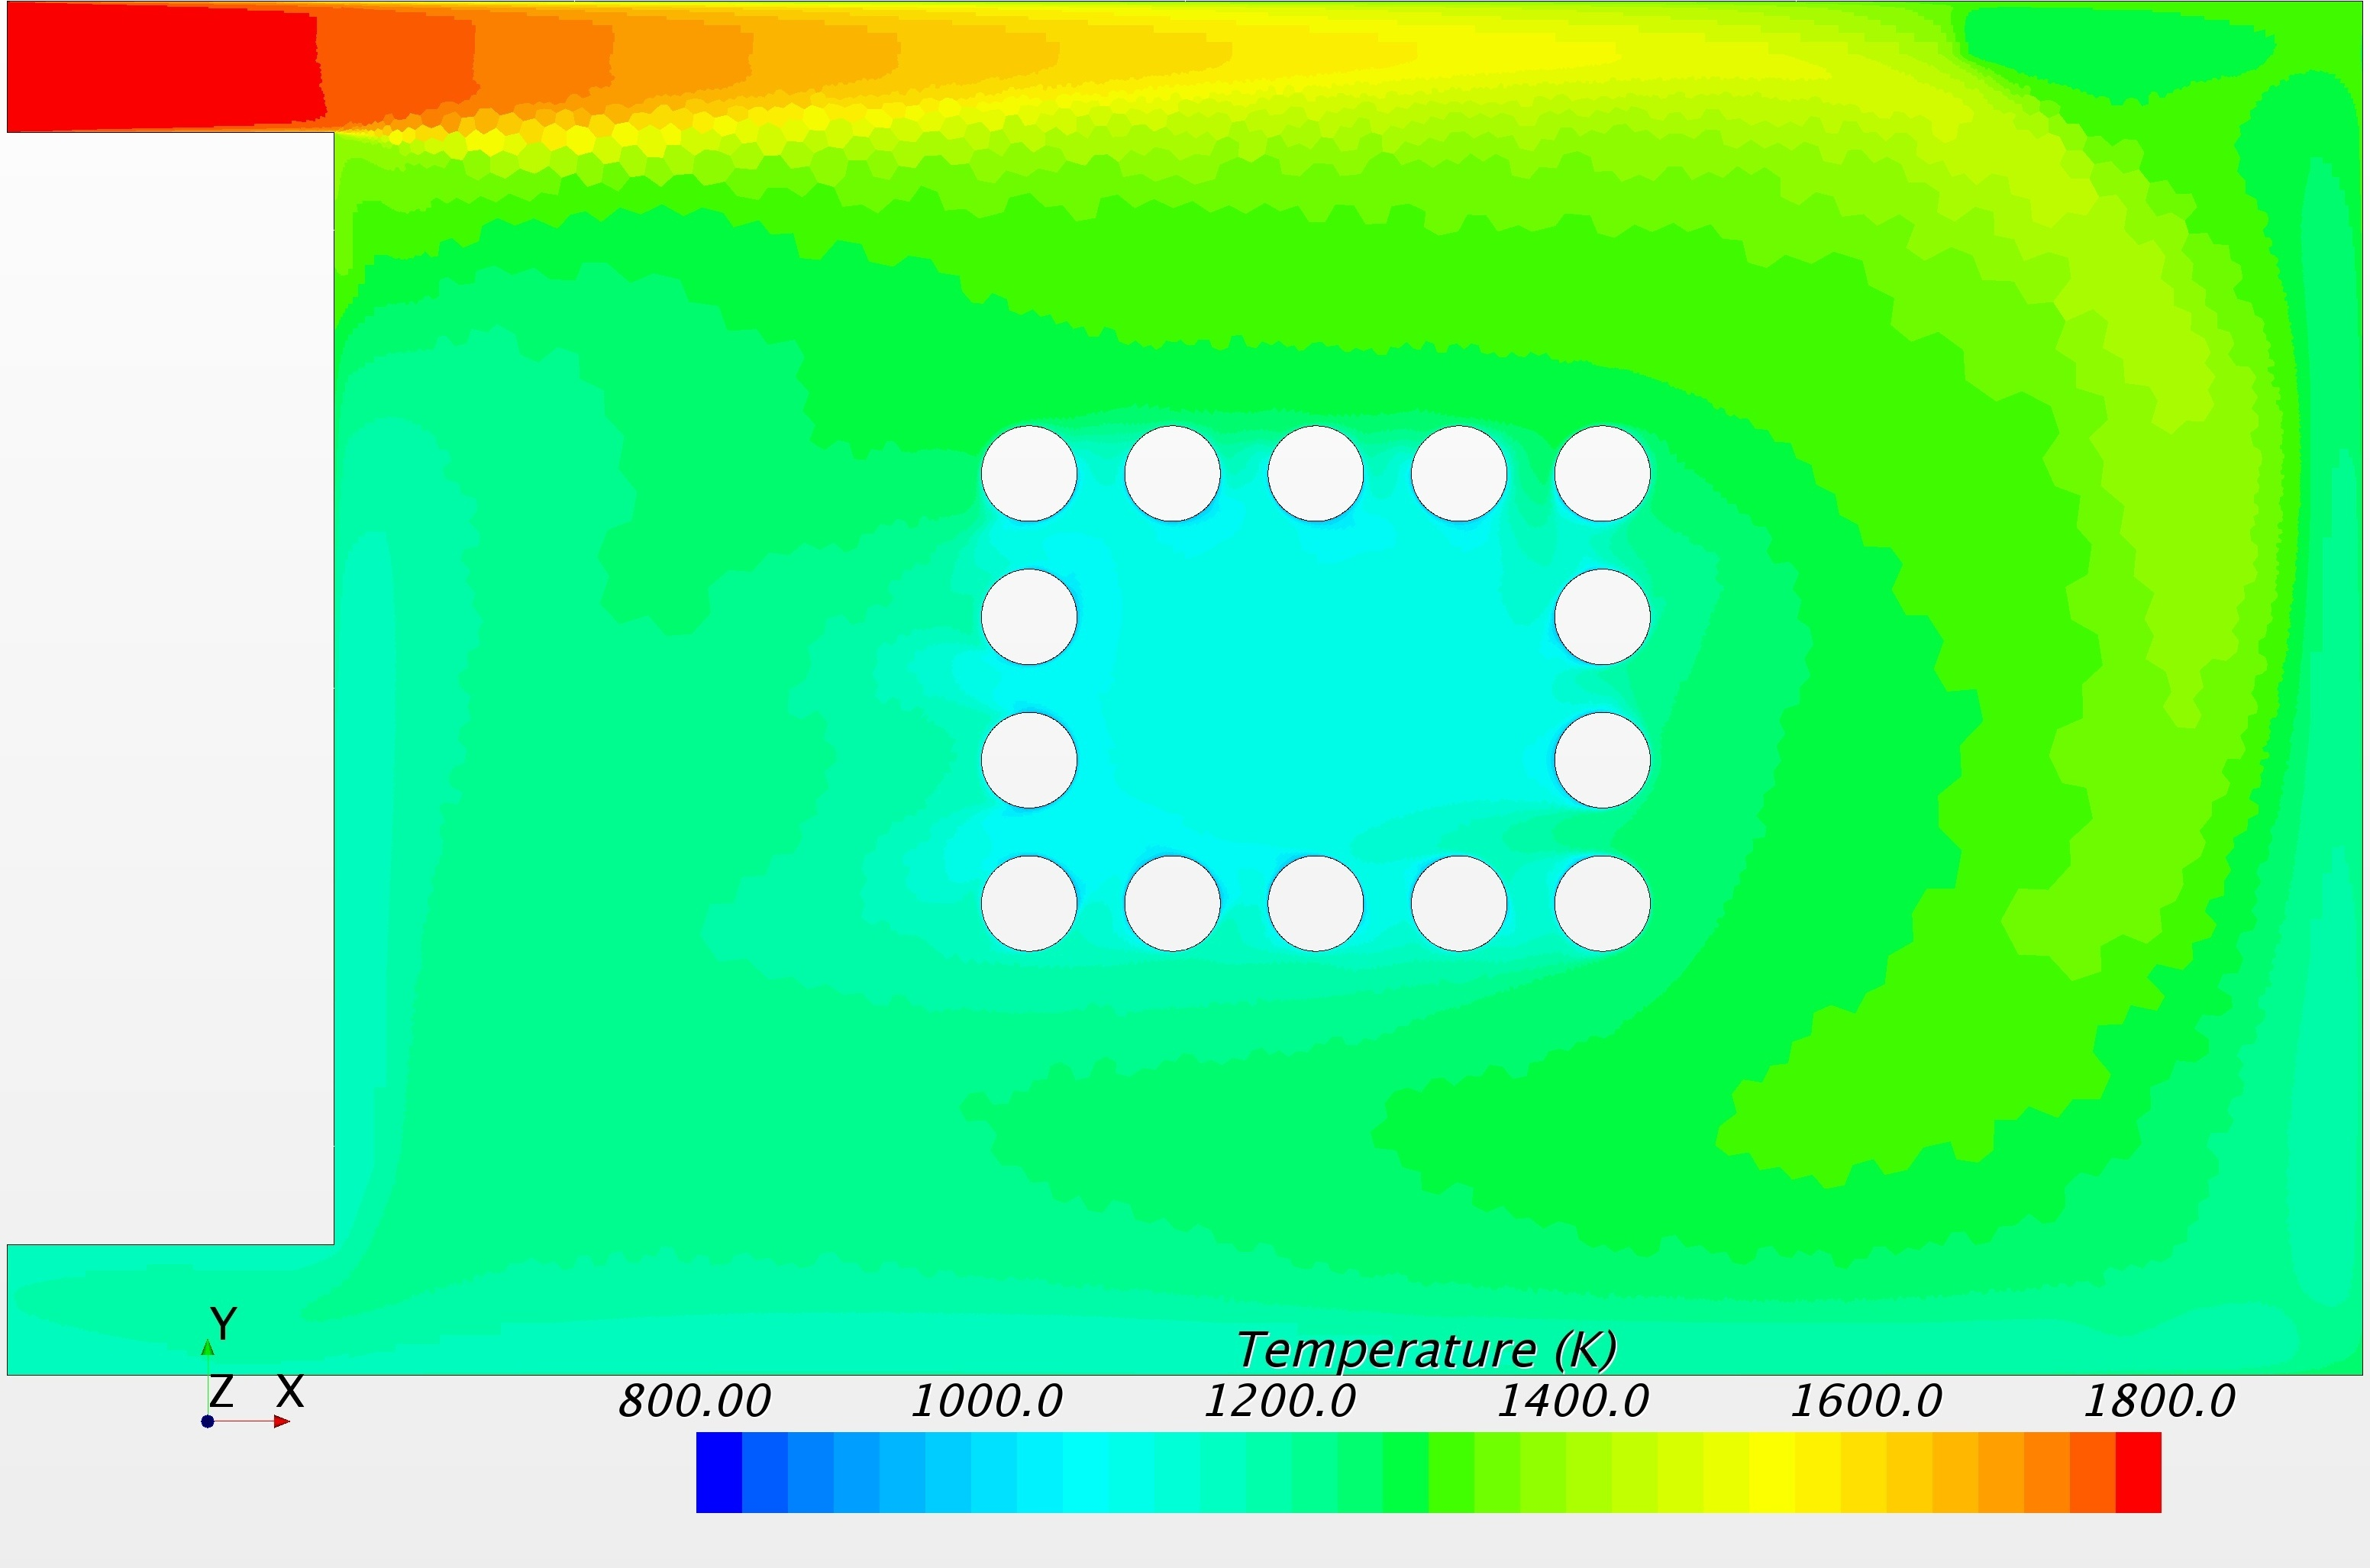
\includegraphics[height=3.8cm]{sources/figure8/c-temp_2.jpg}};
\node (n3b)  [right=0.05cm of n3a]   {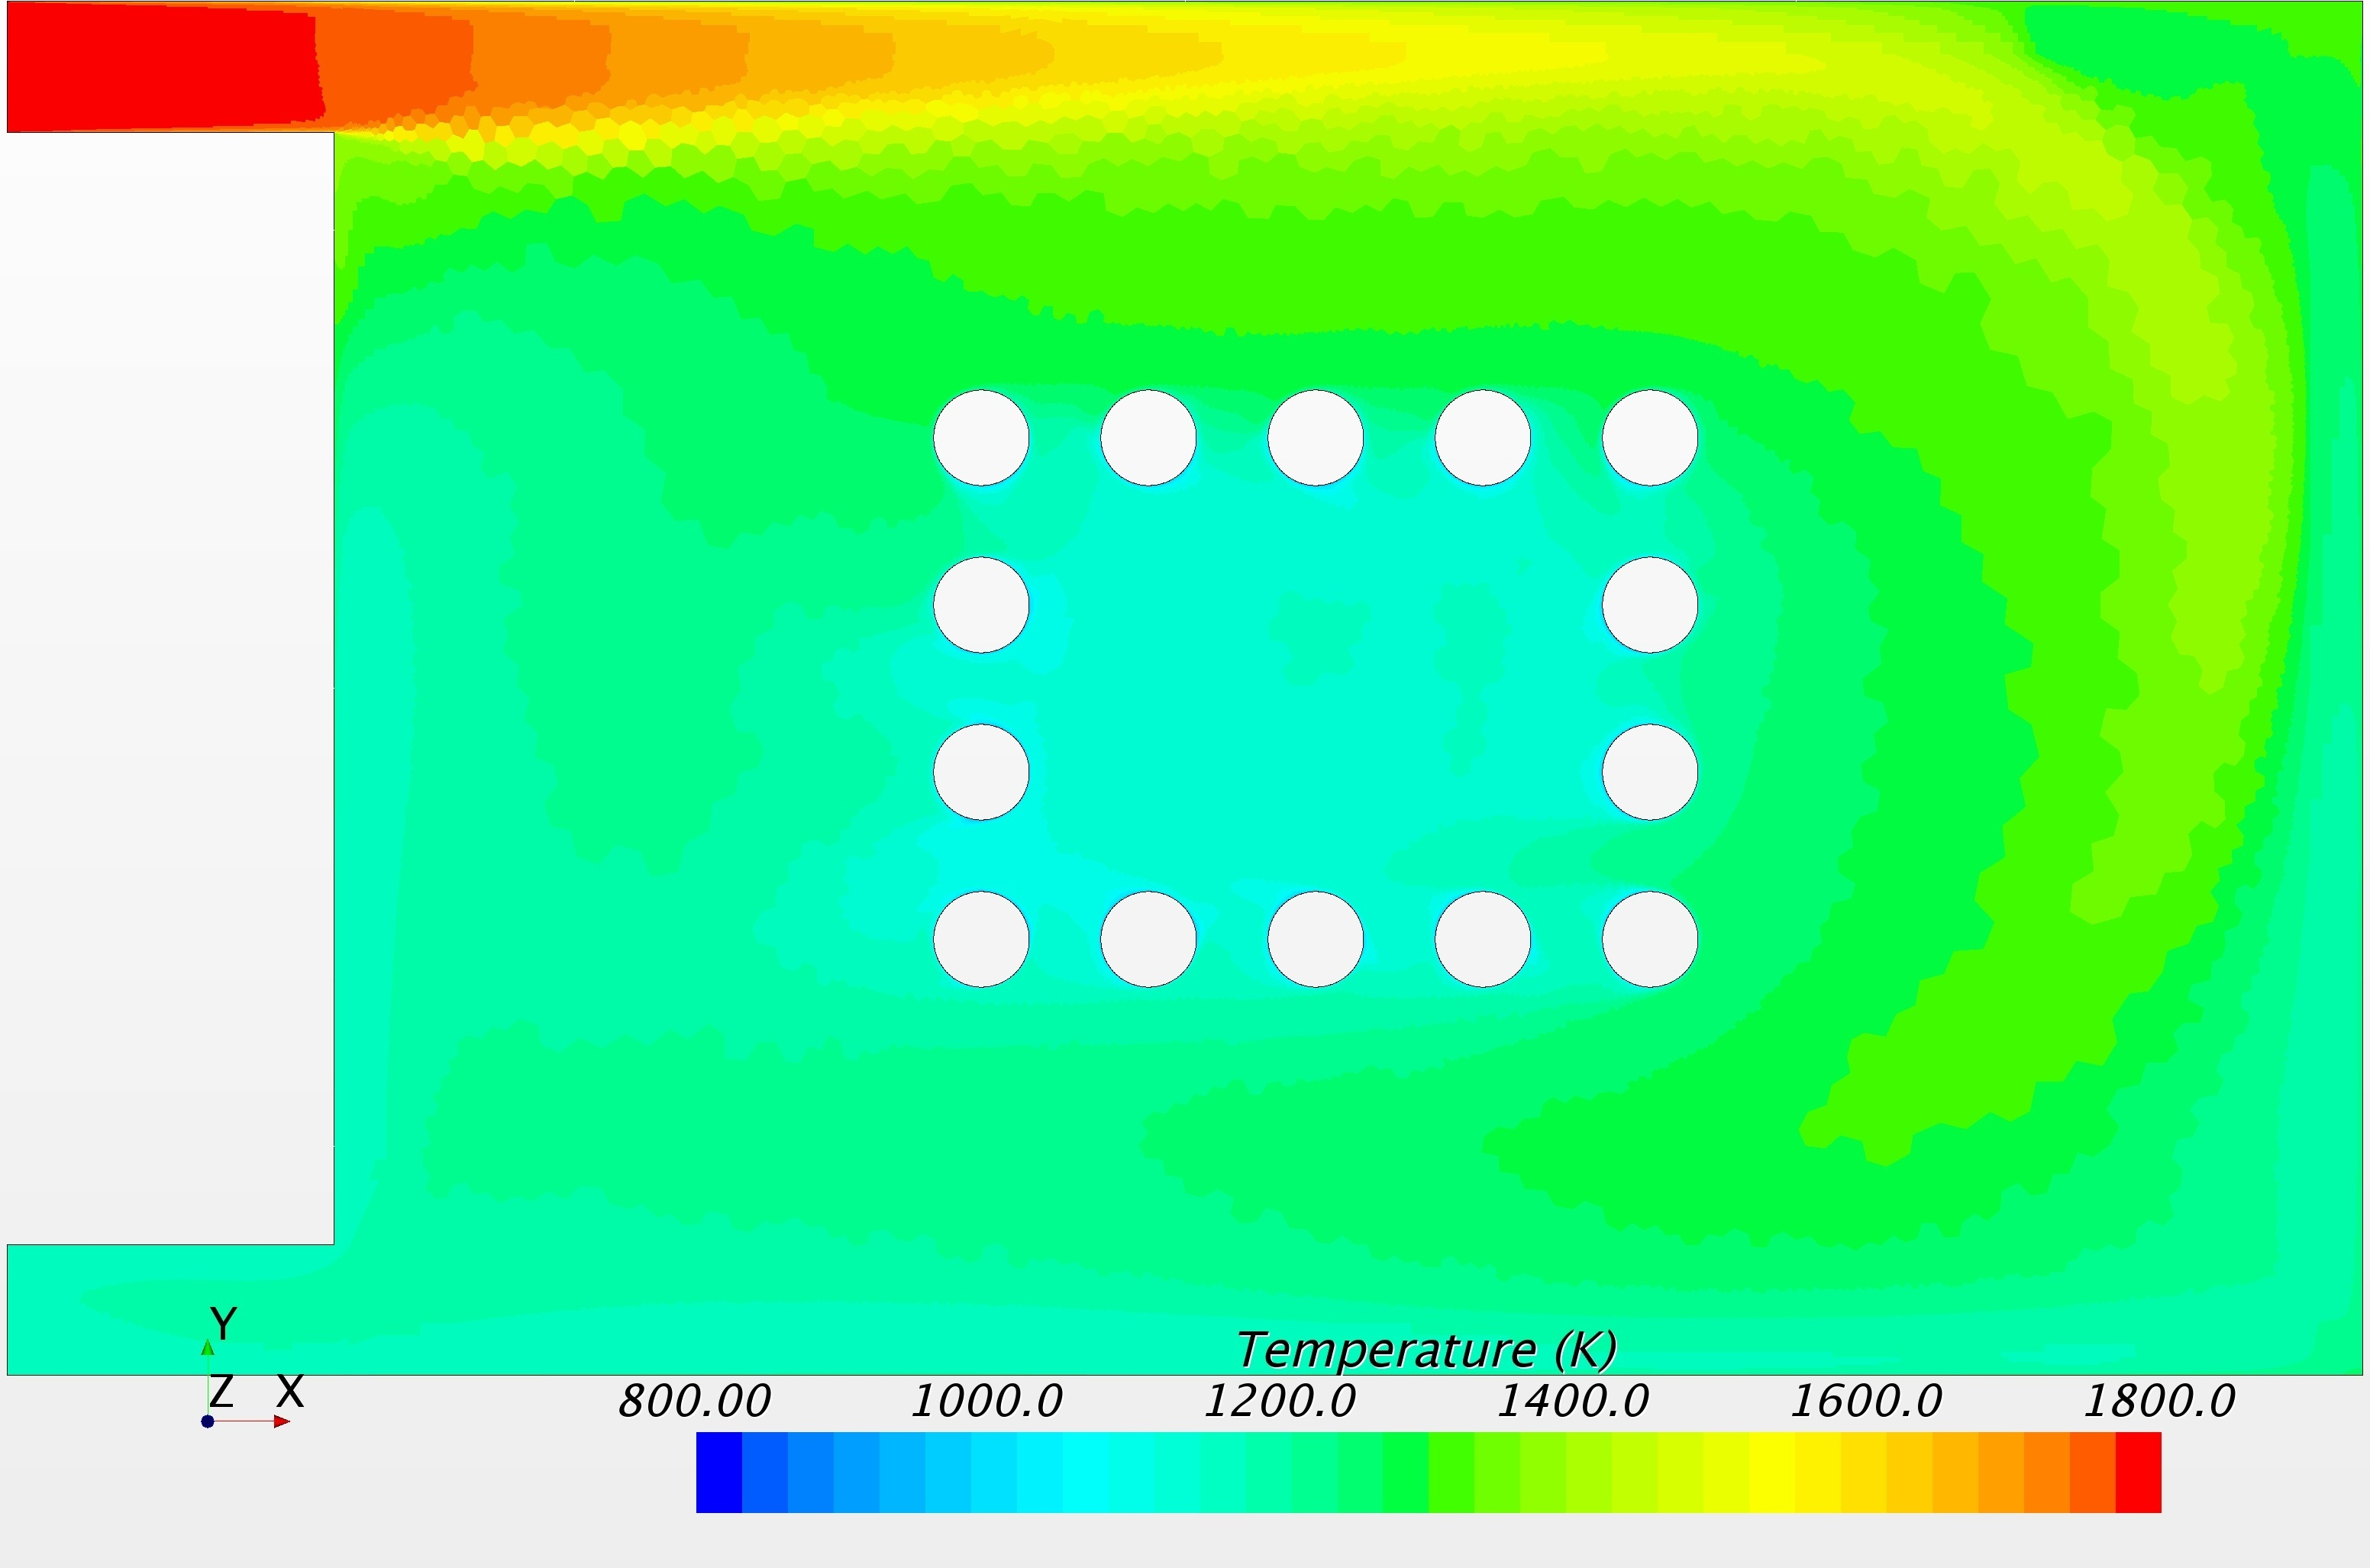
\includegraphics[height=3.8cm]{sources/figure8/c-temp_3.jpg}};
% \node (n4b)  [right=0.05cm of n4a]   {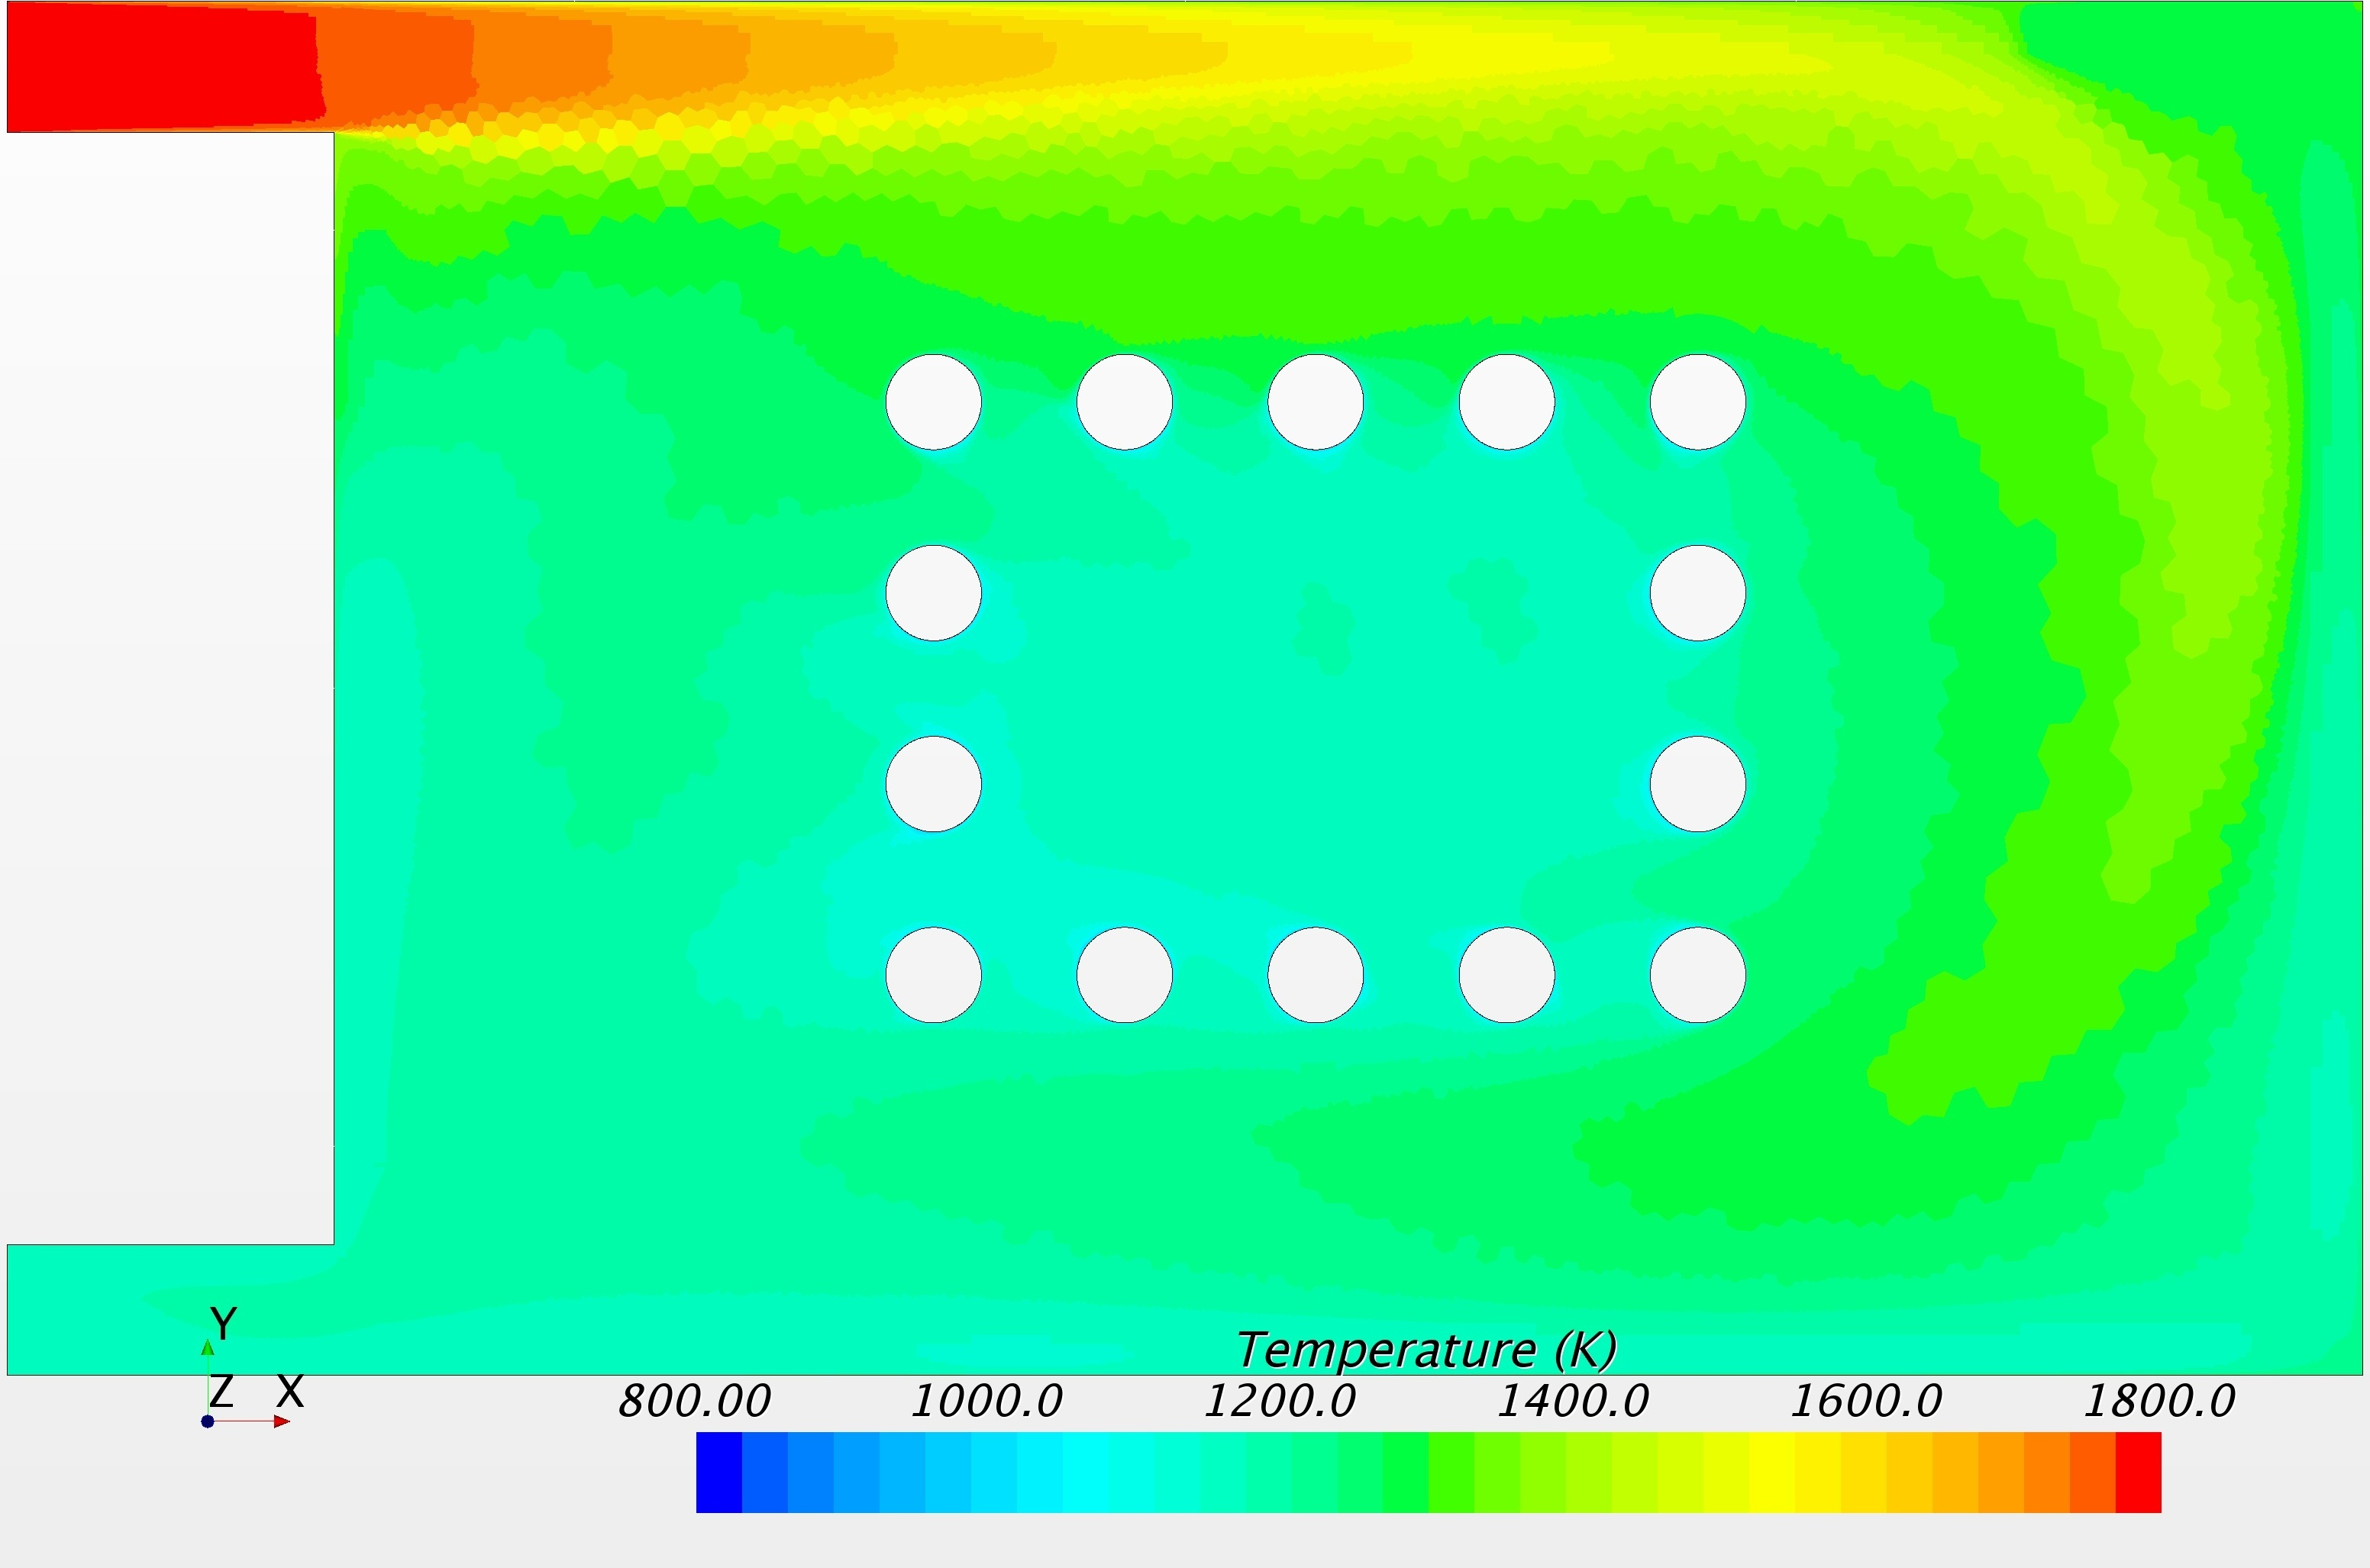
\includegraphics[height=3.8cm]{sources/figure8/c-temp_4.jpg}};
\node (n5b)  [right=0.05cm of n5a]   {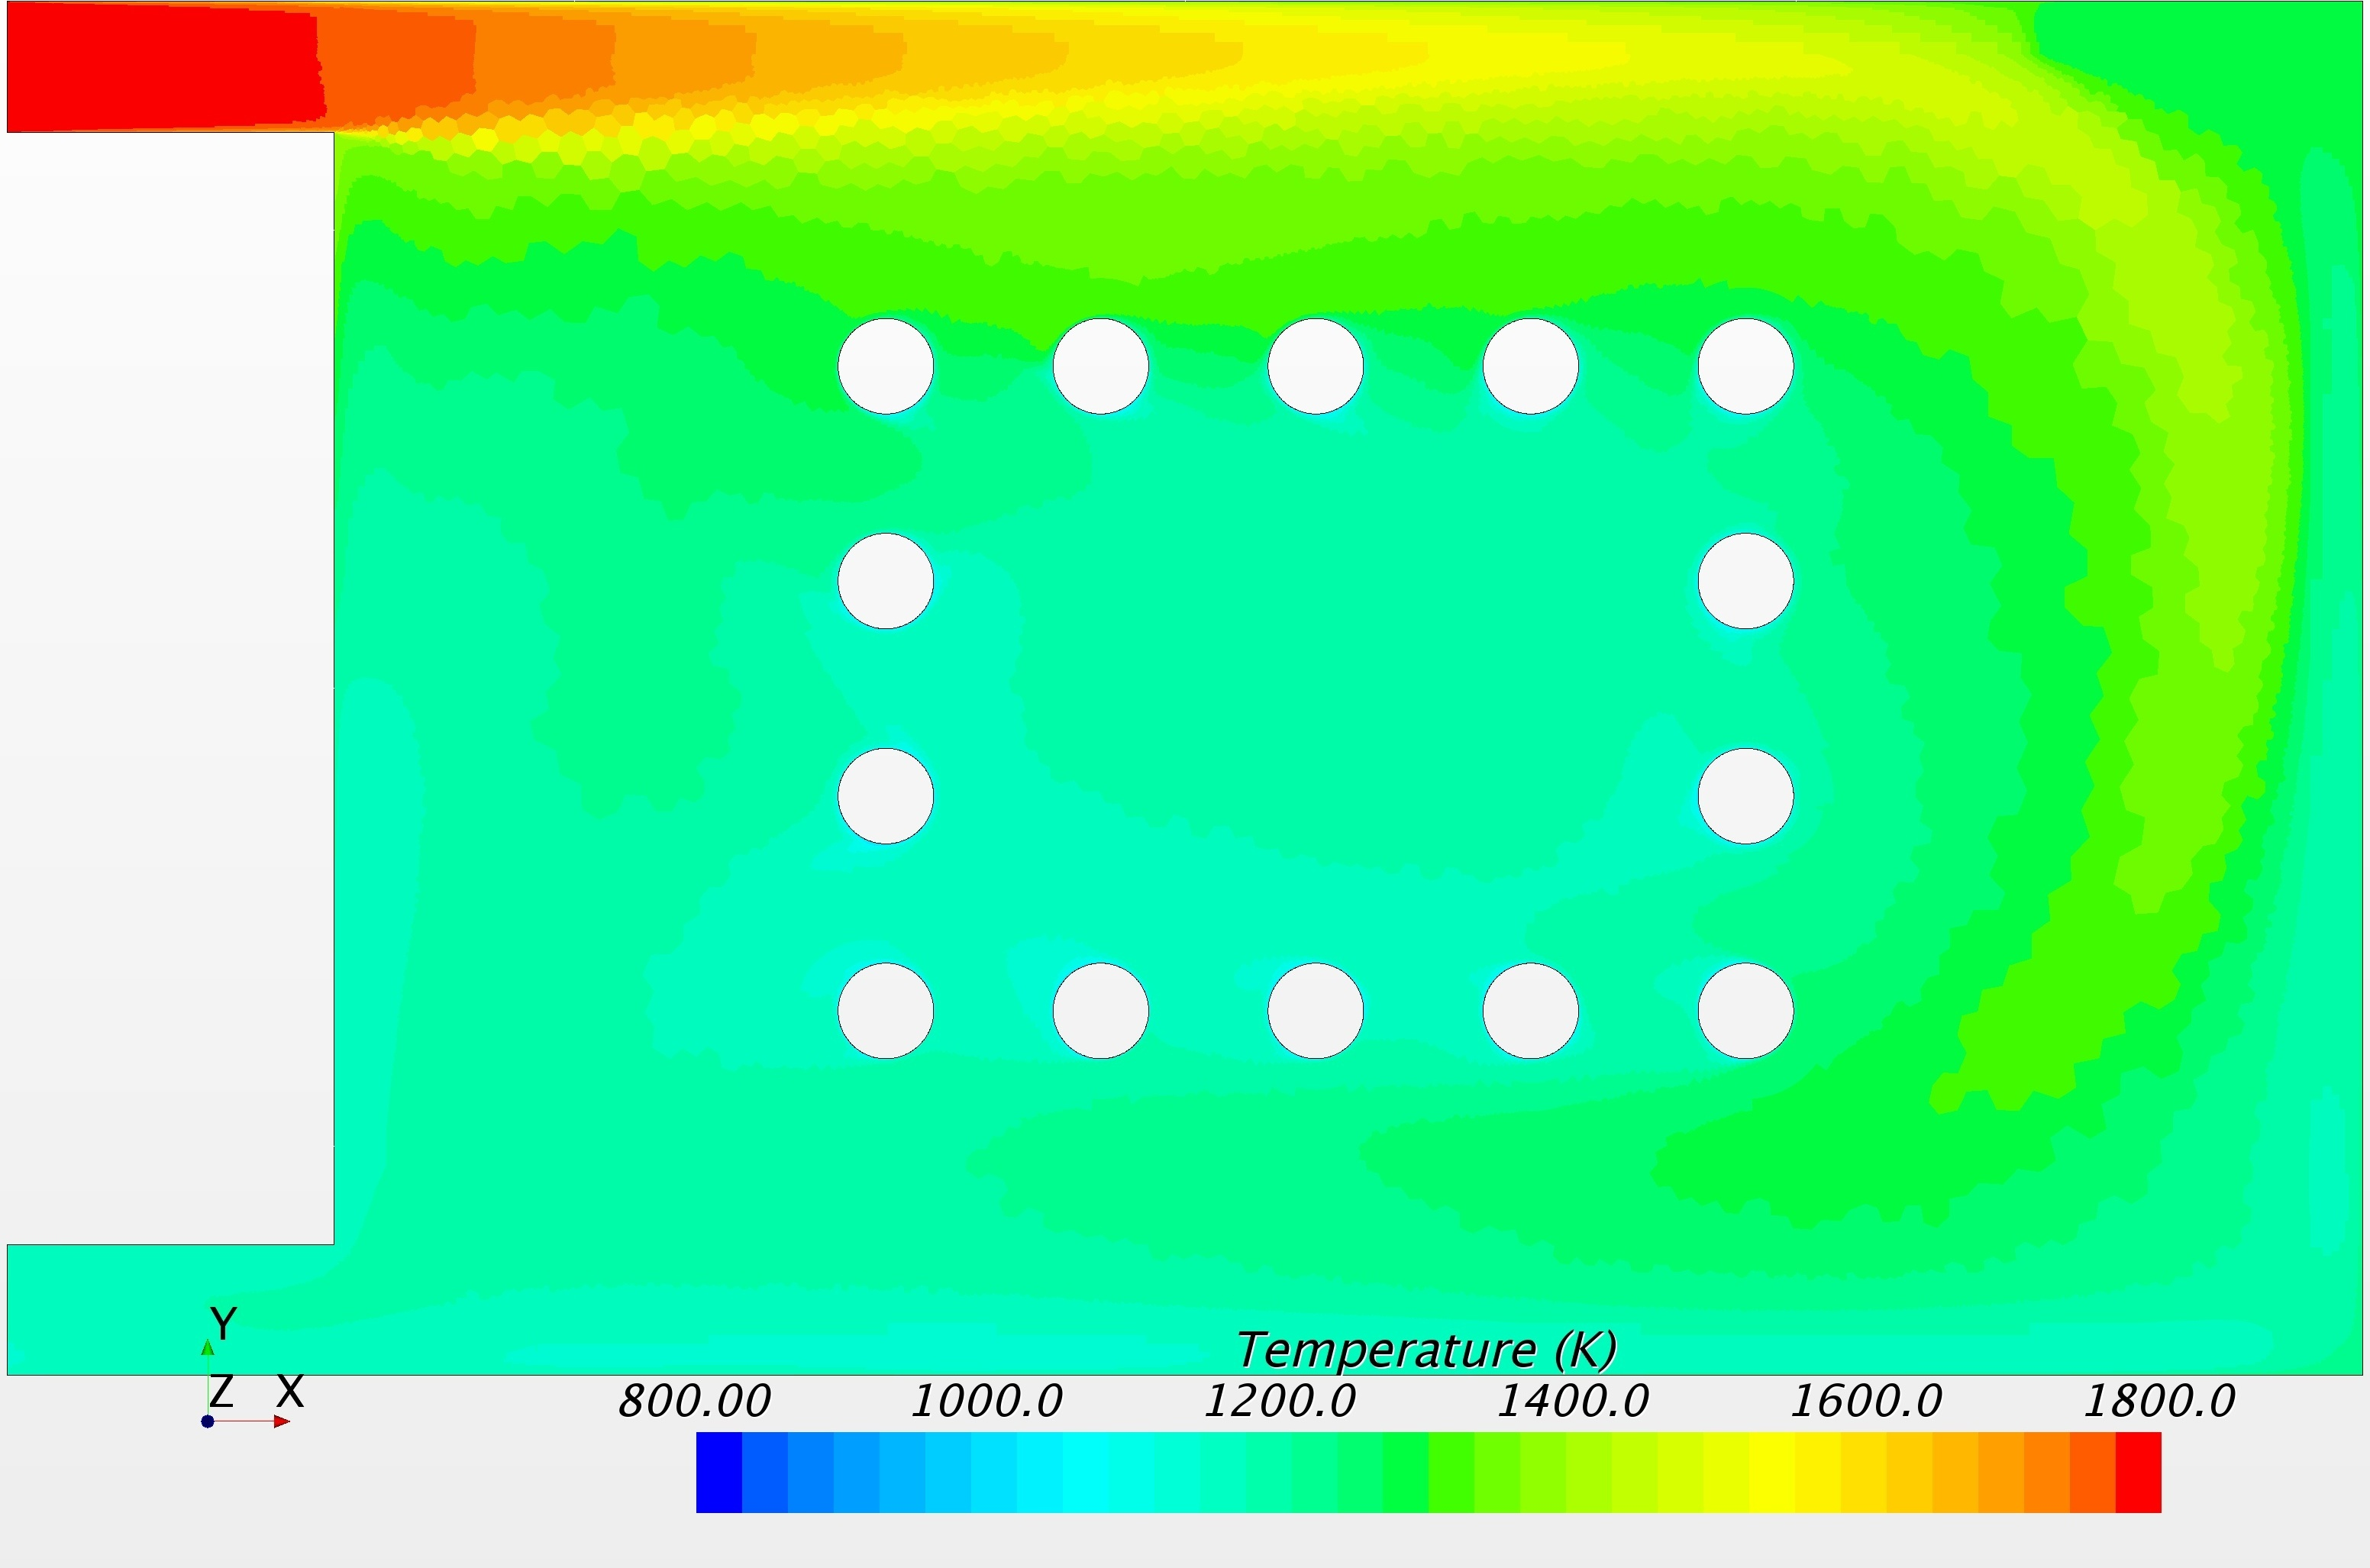
\includegraphics[height=3.8cm]{sources/figure8/c-temp_5.jpg}};
% \node (n6b)  [right=0.05cm of n6a]   {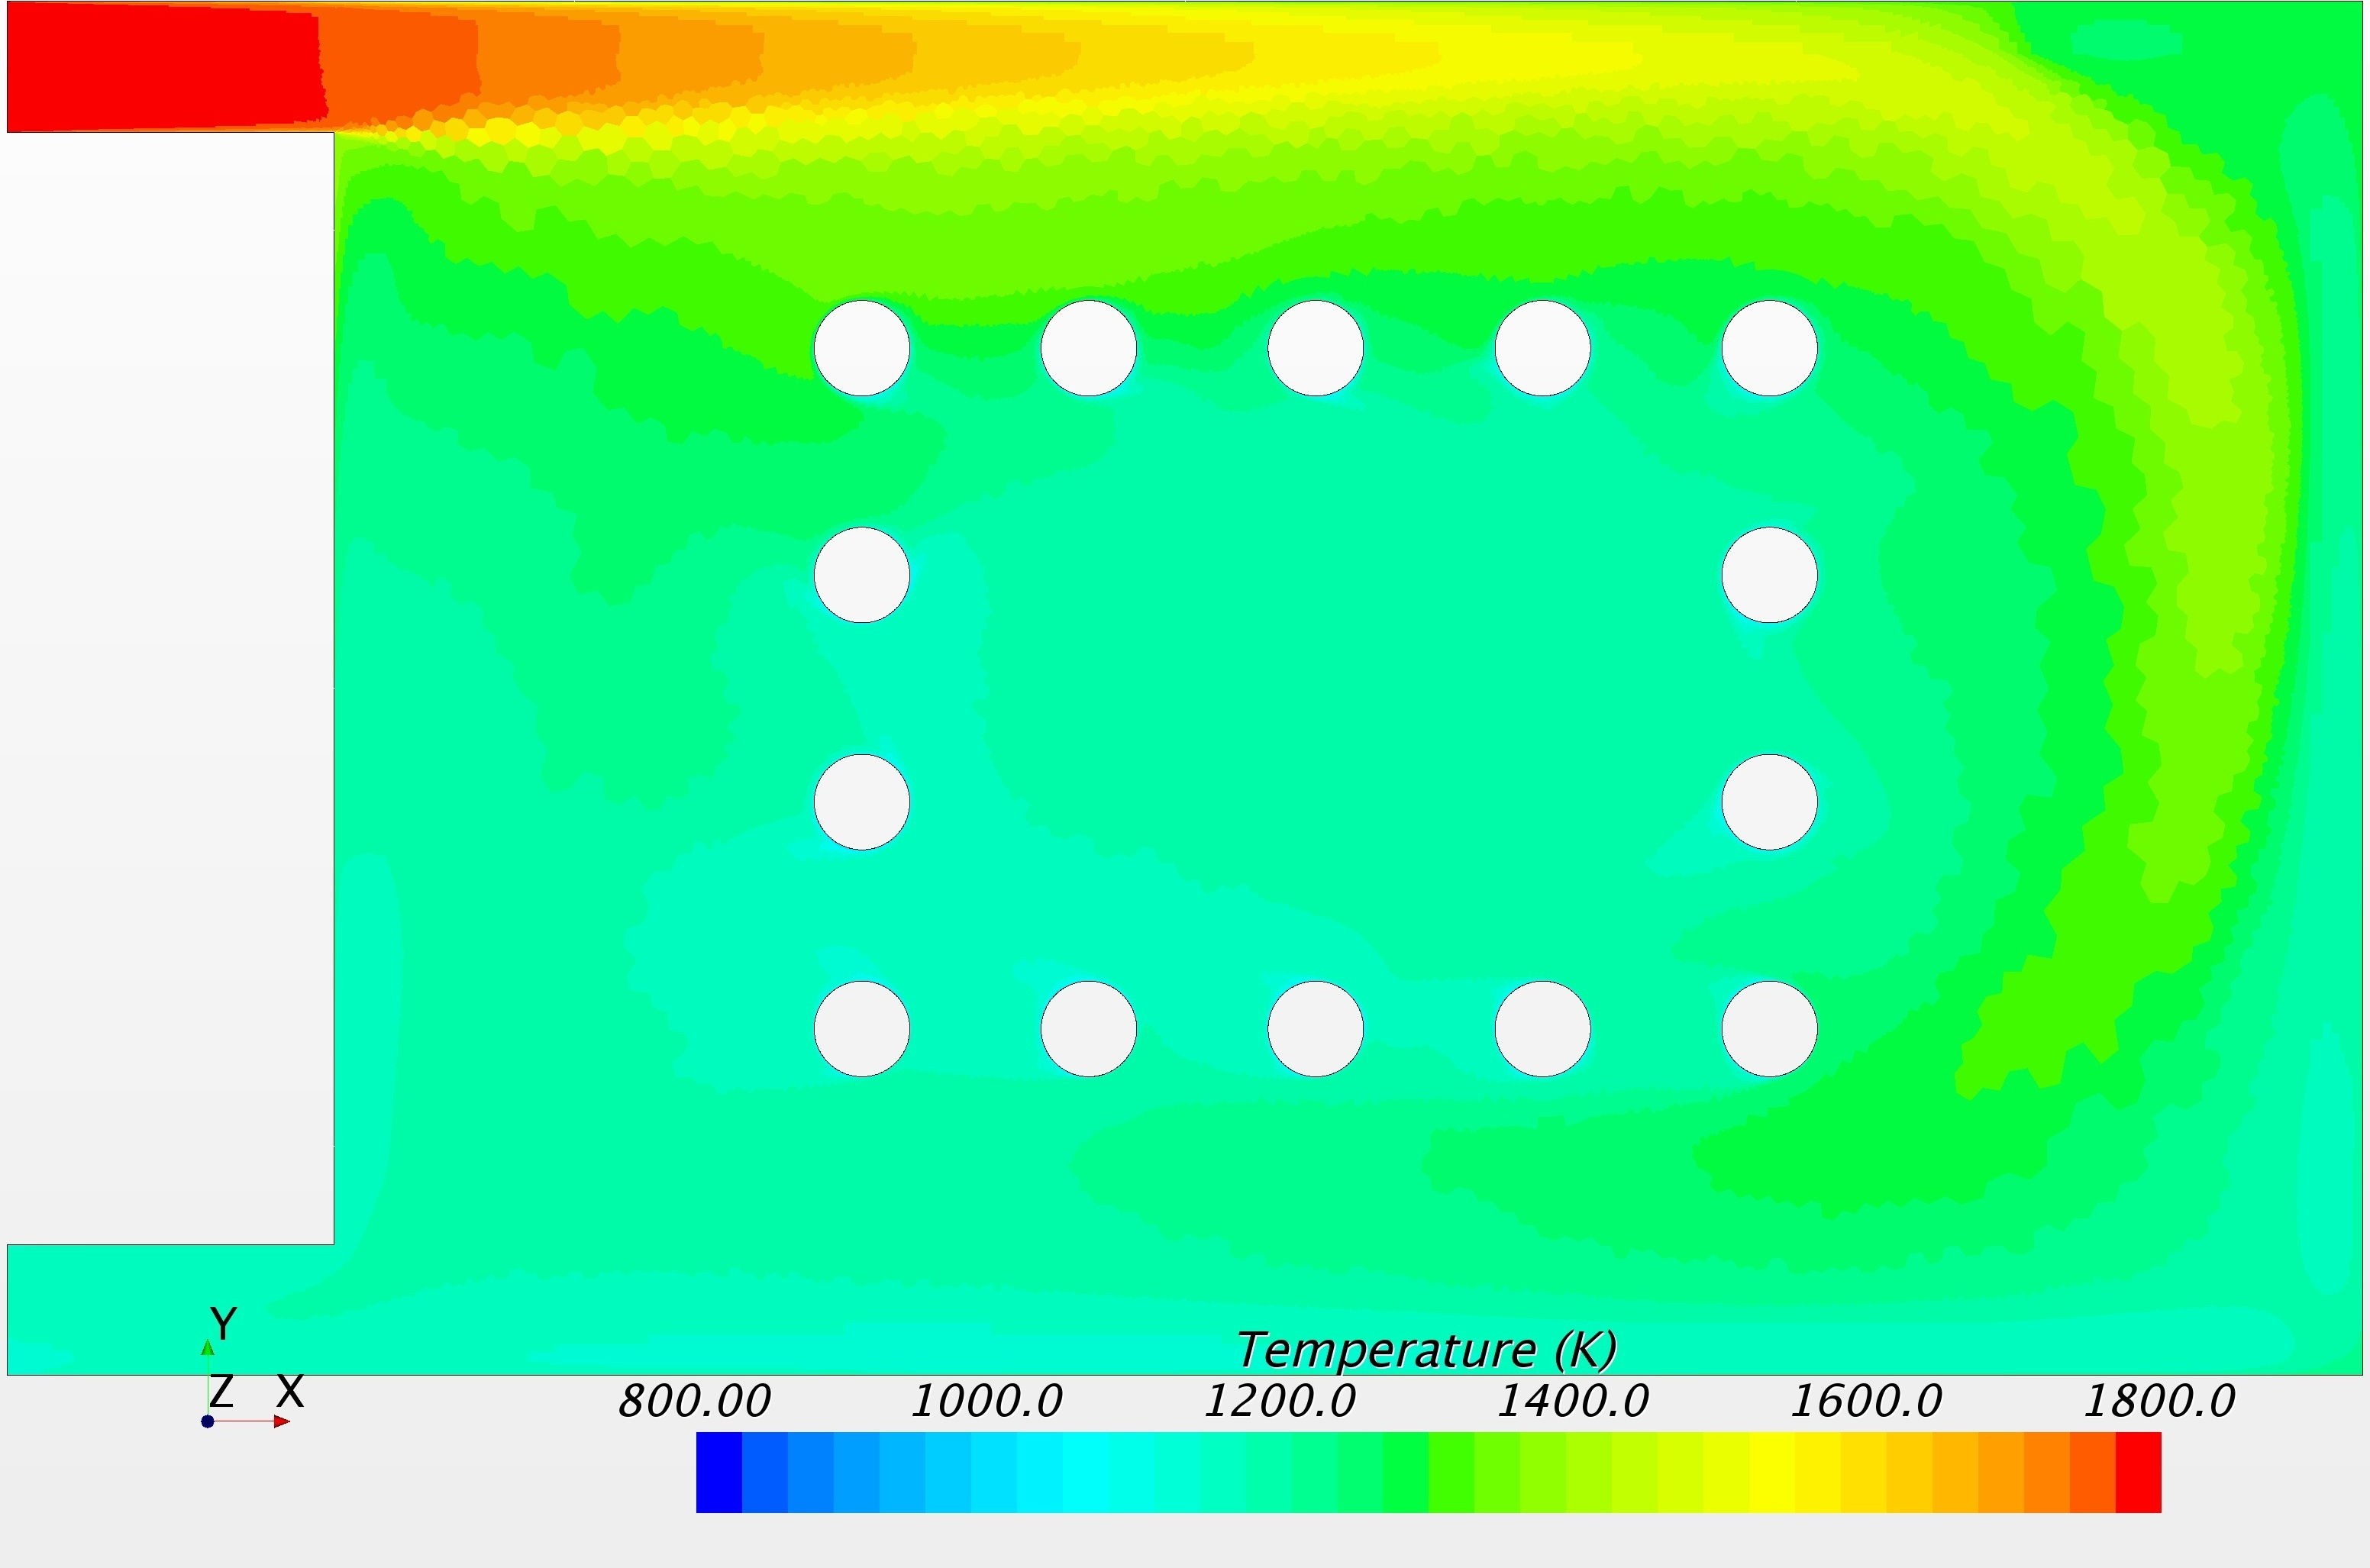
\includegraphics[height=3.8cm]{sources/figure8/c-temp_6.jpg}};
\node (n7b)  [right=0.05cm of n7a]   {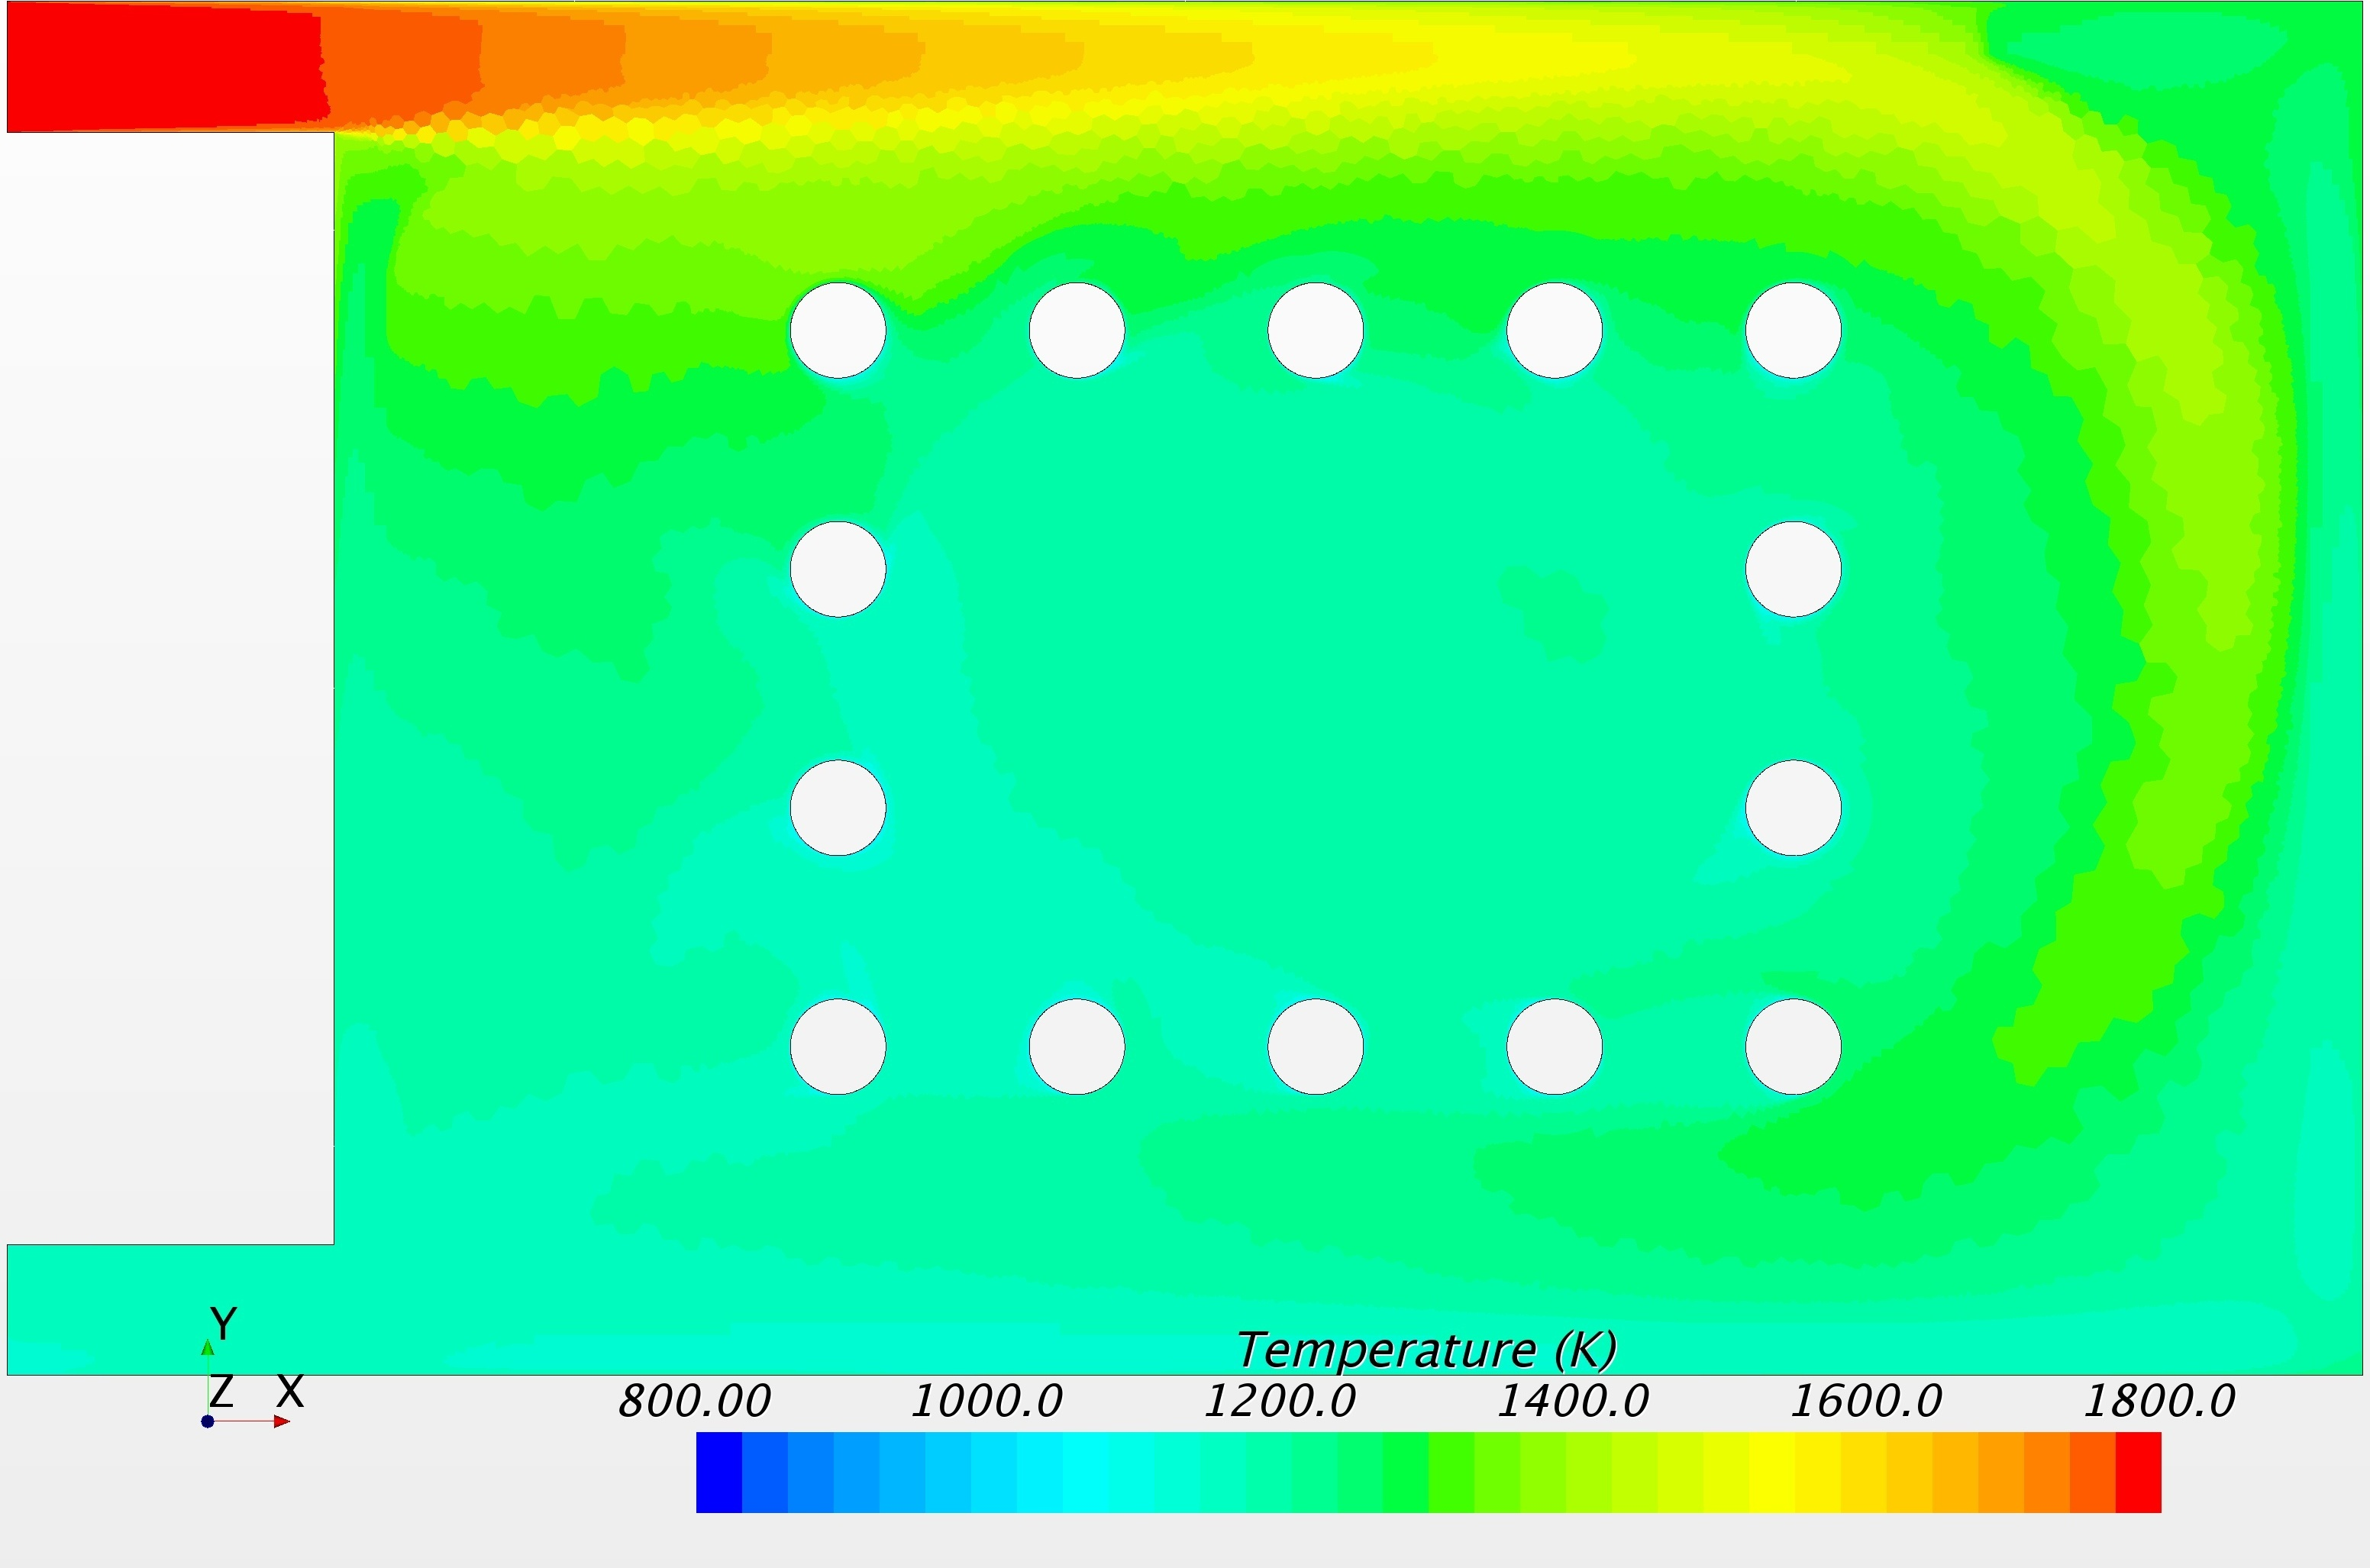
\includegraphics[height=3.8cm]{sources/figure8/c-temp_7.jpg}};
% \node (n8b)  [right=0.05cm of n8a]   {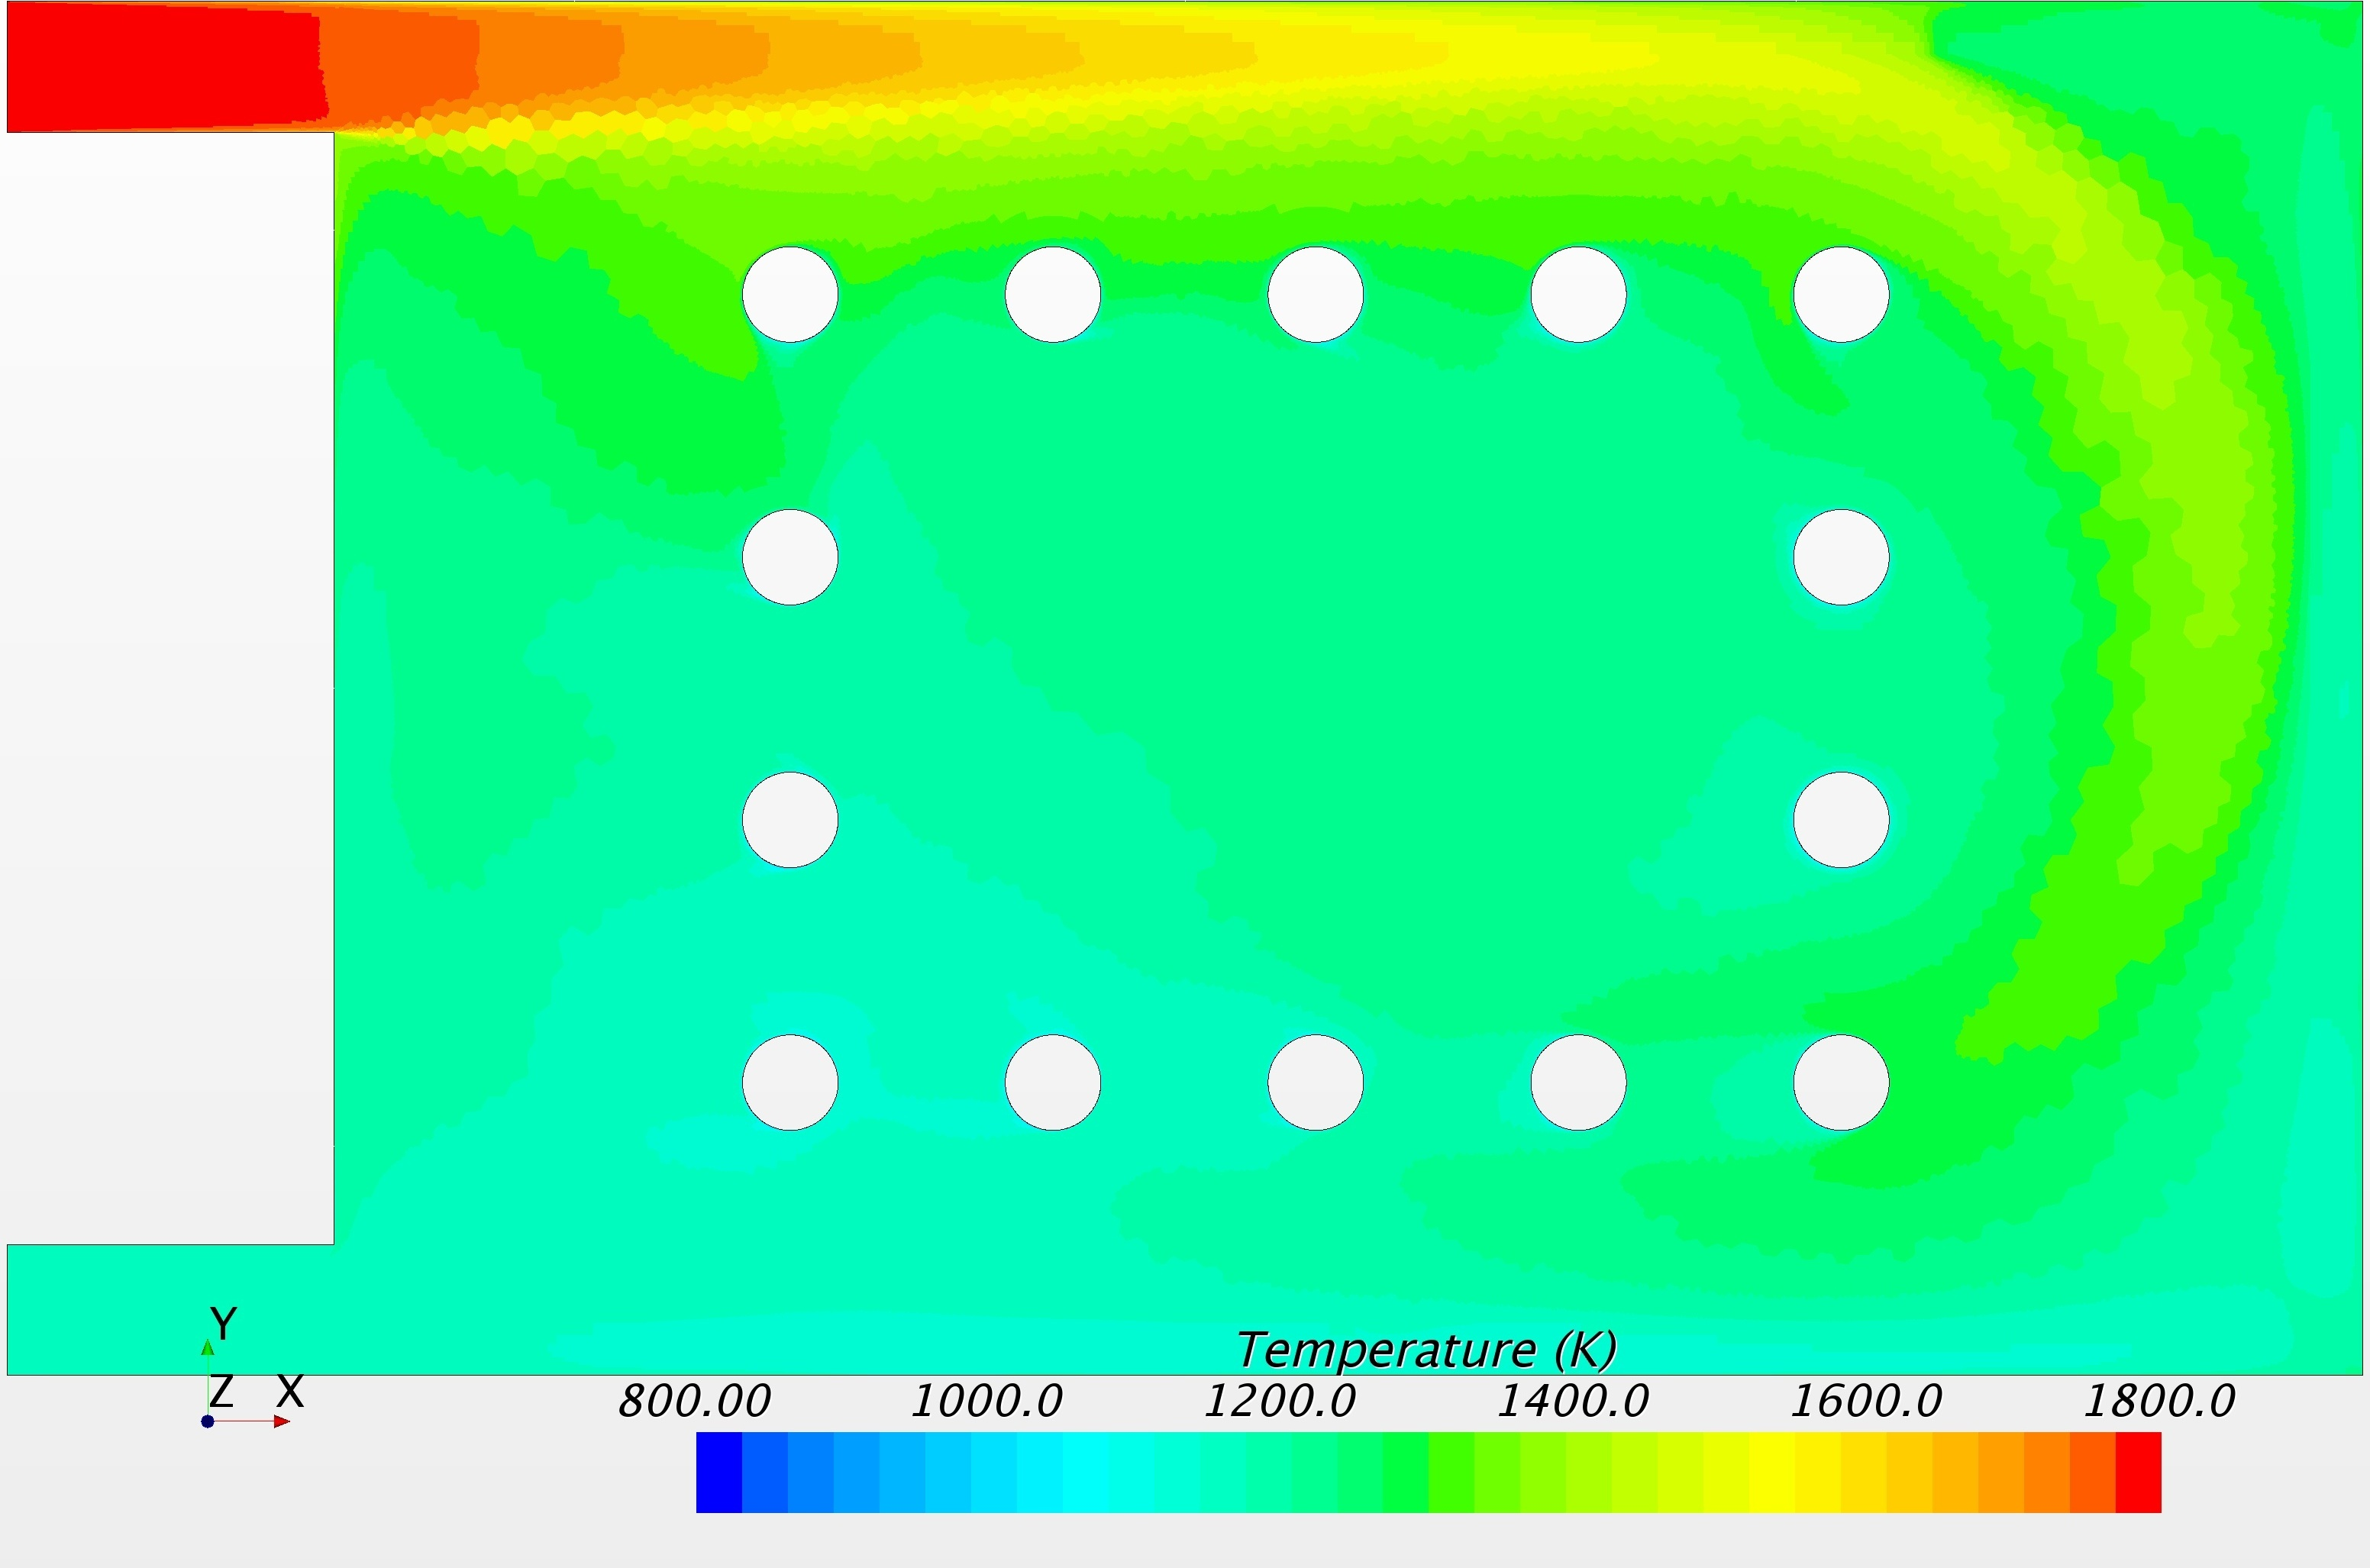
\includegraphics[height=3.8cm]{sources/figure8/c-temp_8.jpg}};
% \node (n9b)  [right=0.05cm of n9a]   {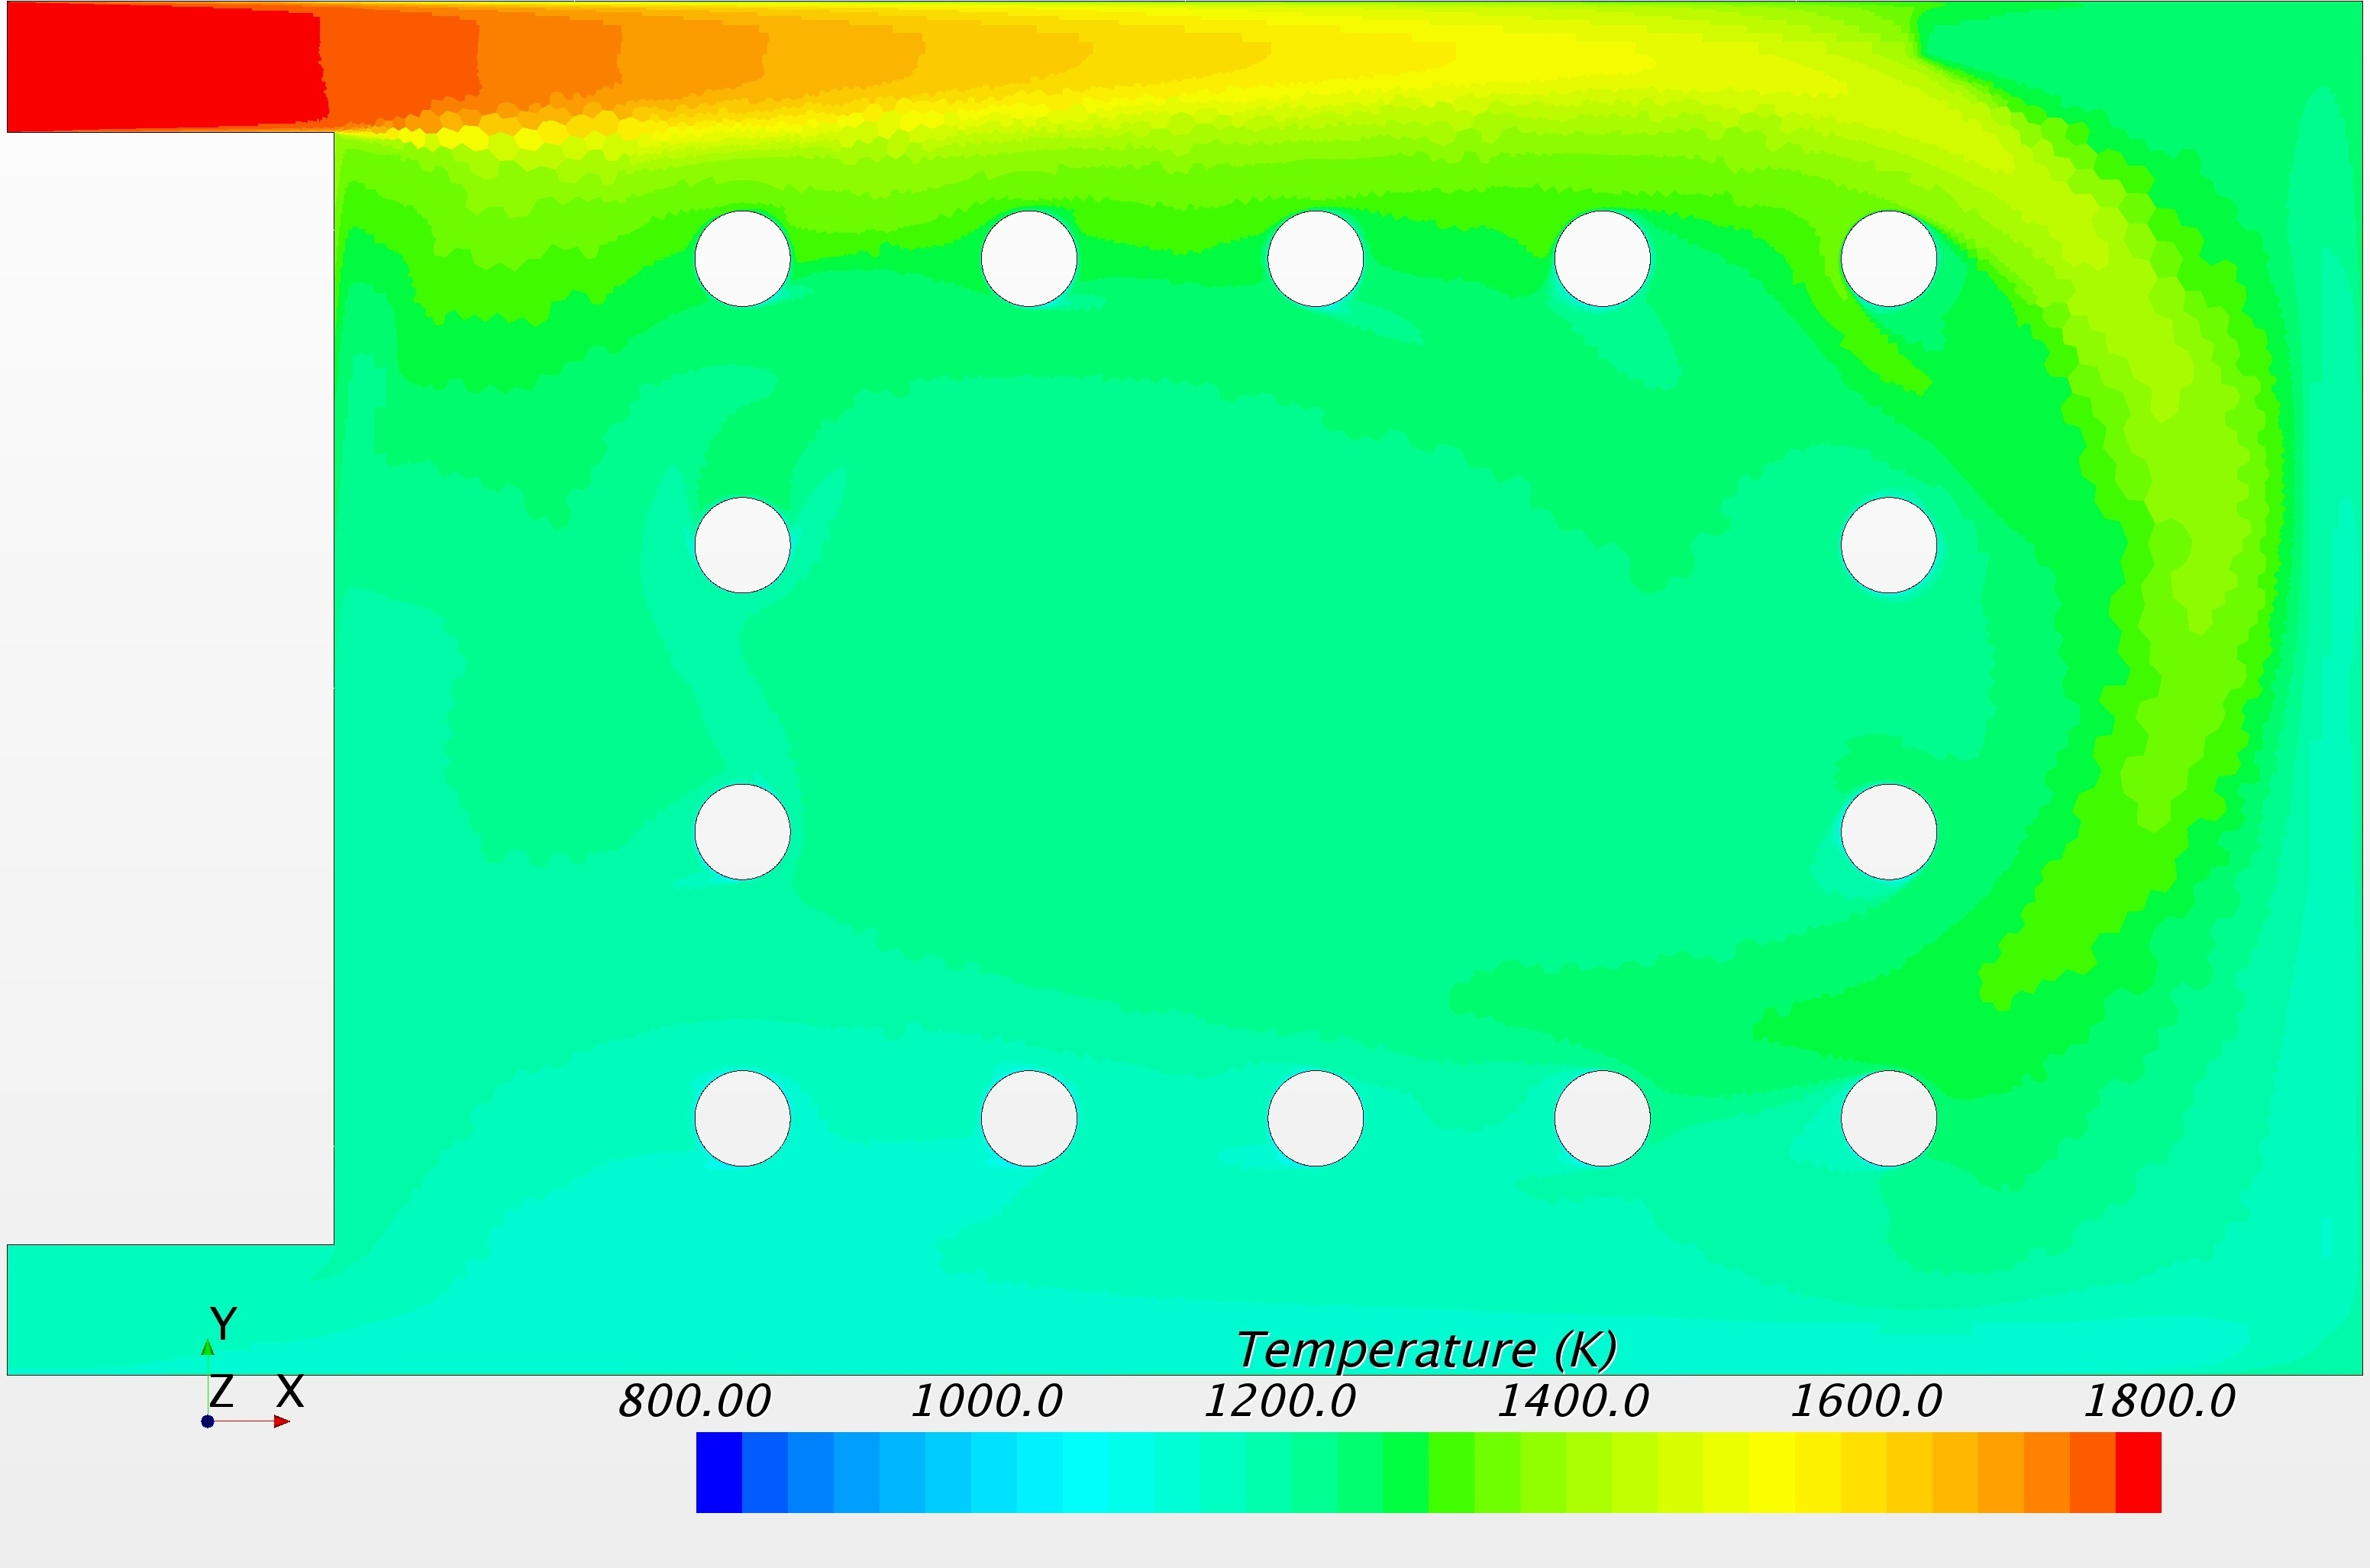
\includegraphics[height=3.8cm]{sources/figure8/c-temp_9.jpg}};
\node (n10b) [right=0.05cm of n10a]  {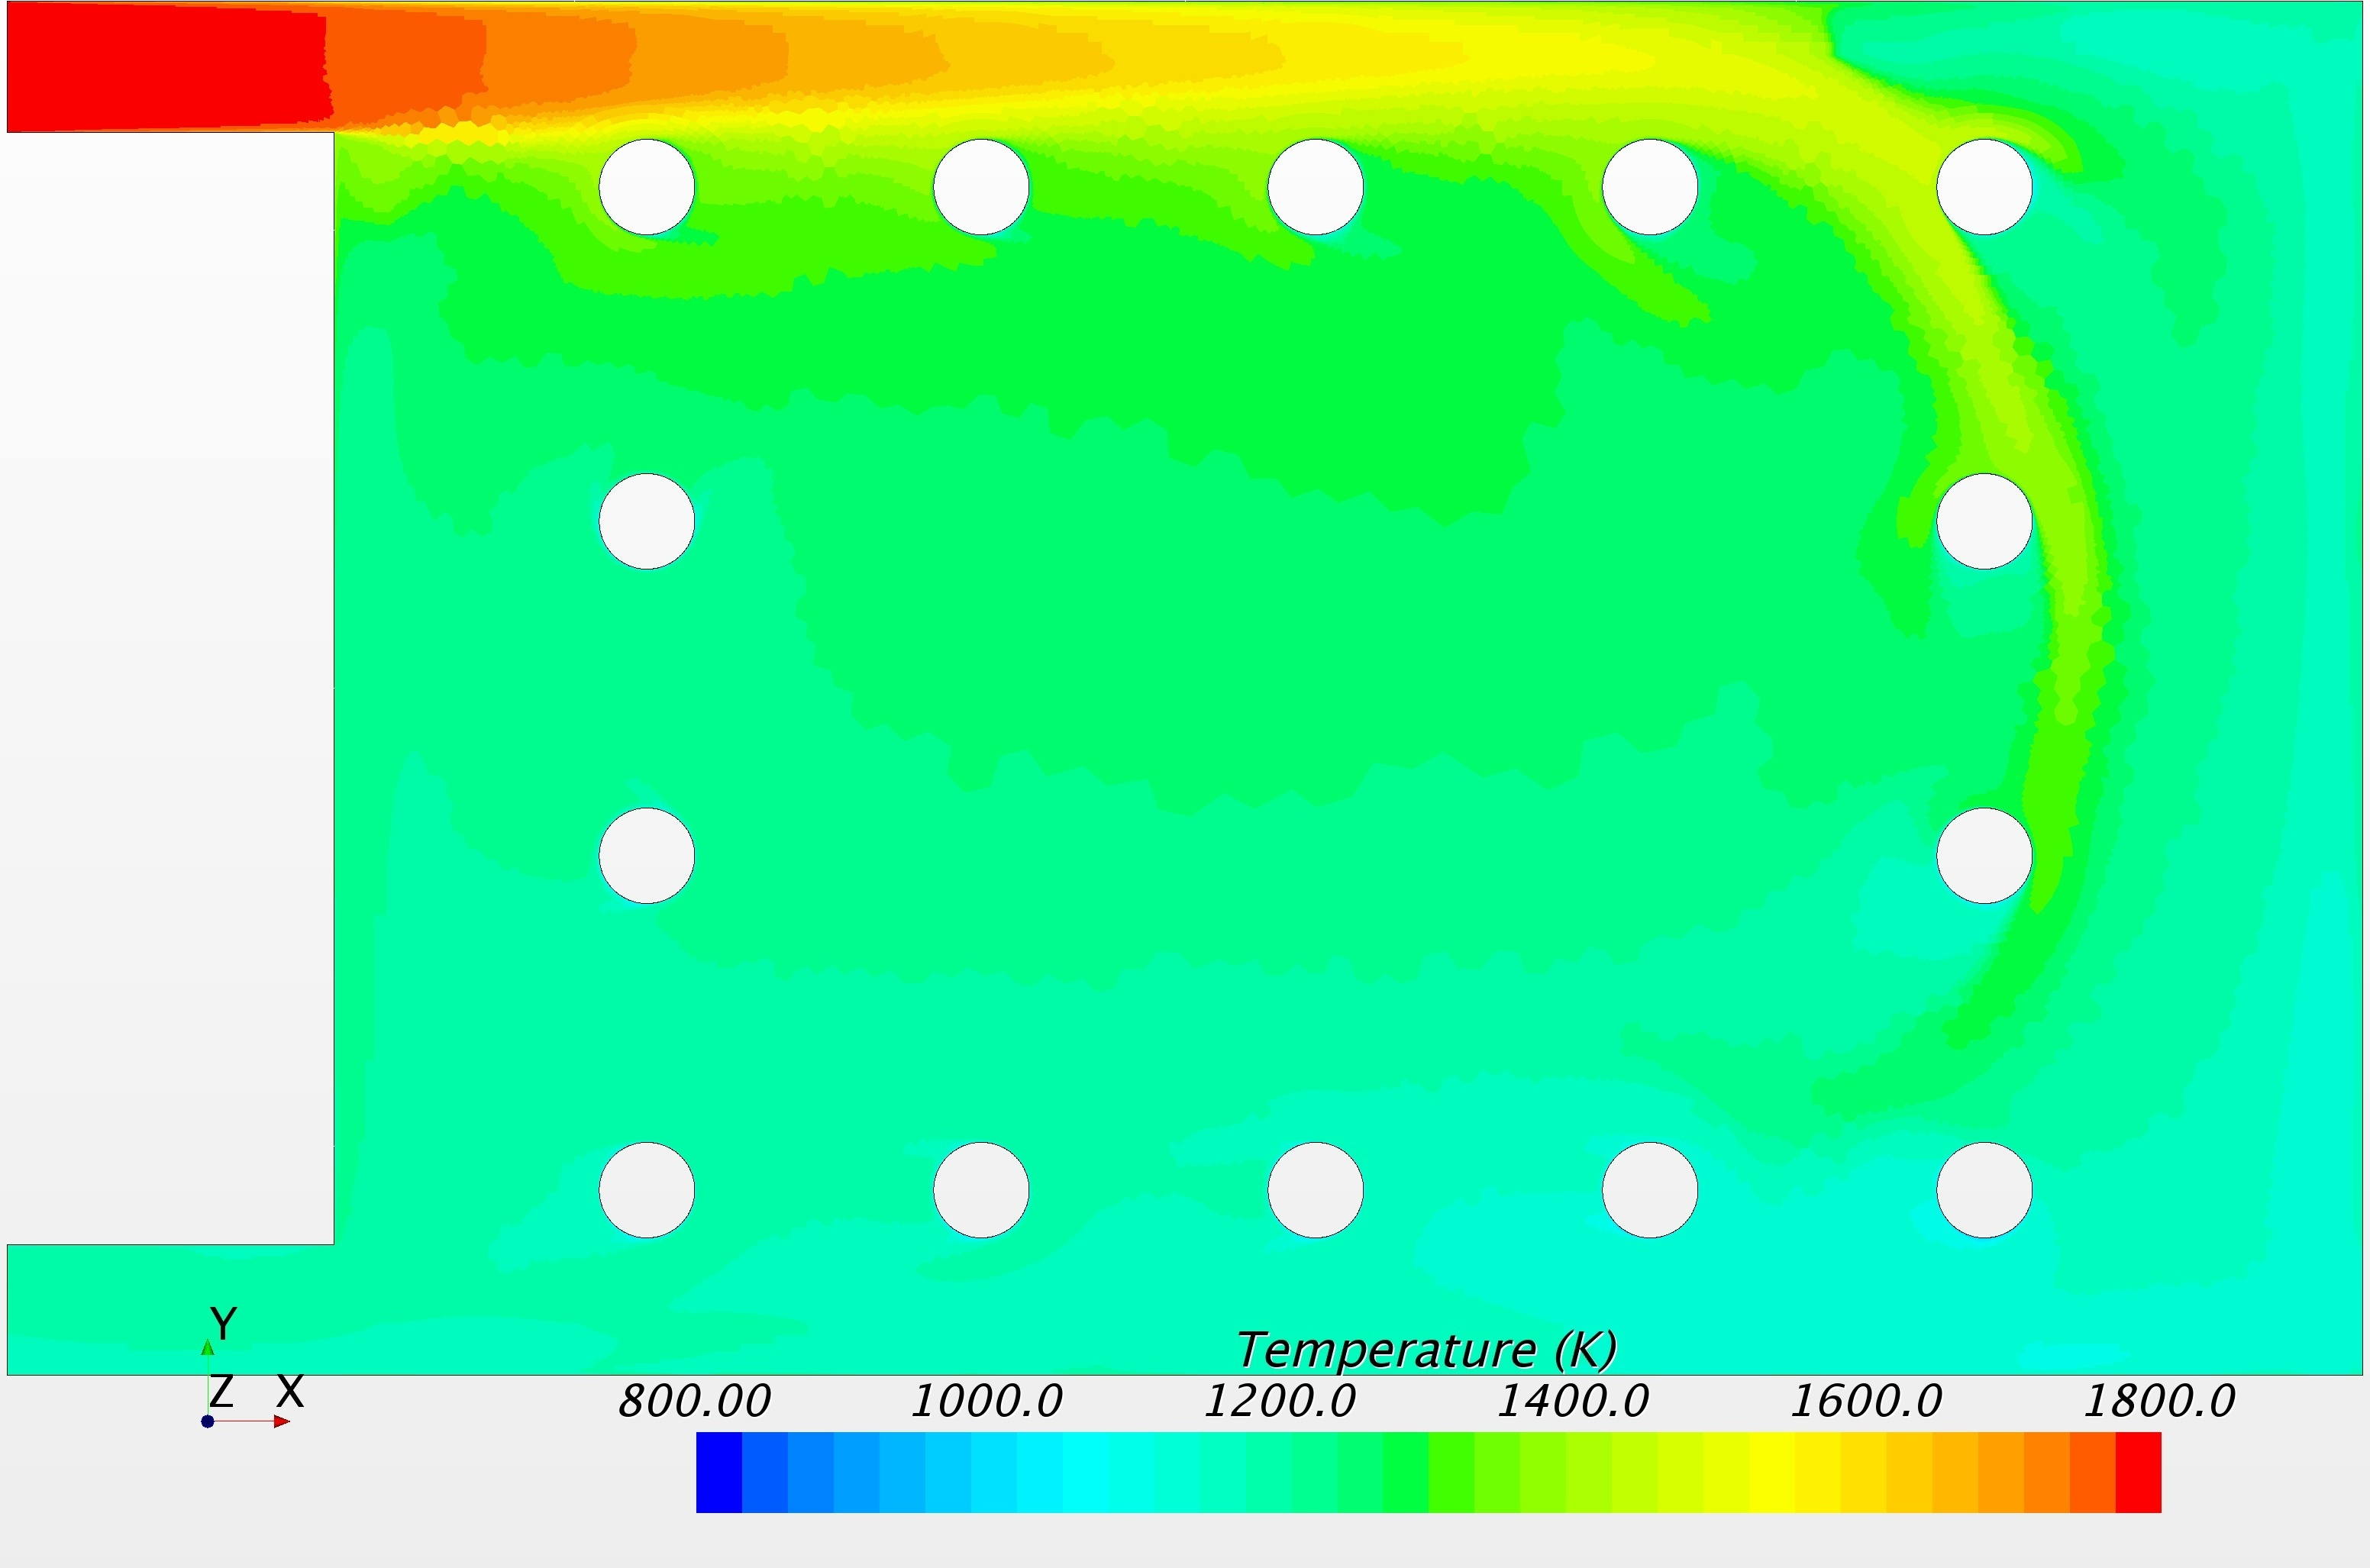
\includegraphics[height=3.8cm]{sources/figure8/c-temp_10.jpg}};
\node (n11b) [right=0.05cm of n11a]  {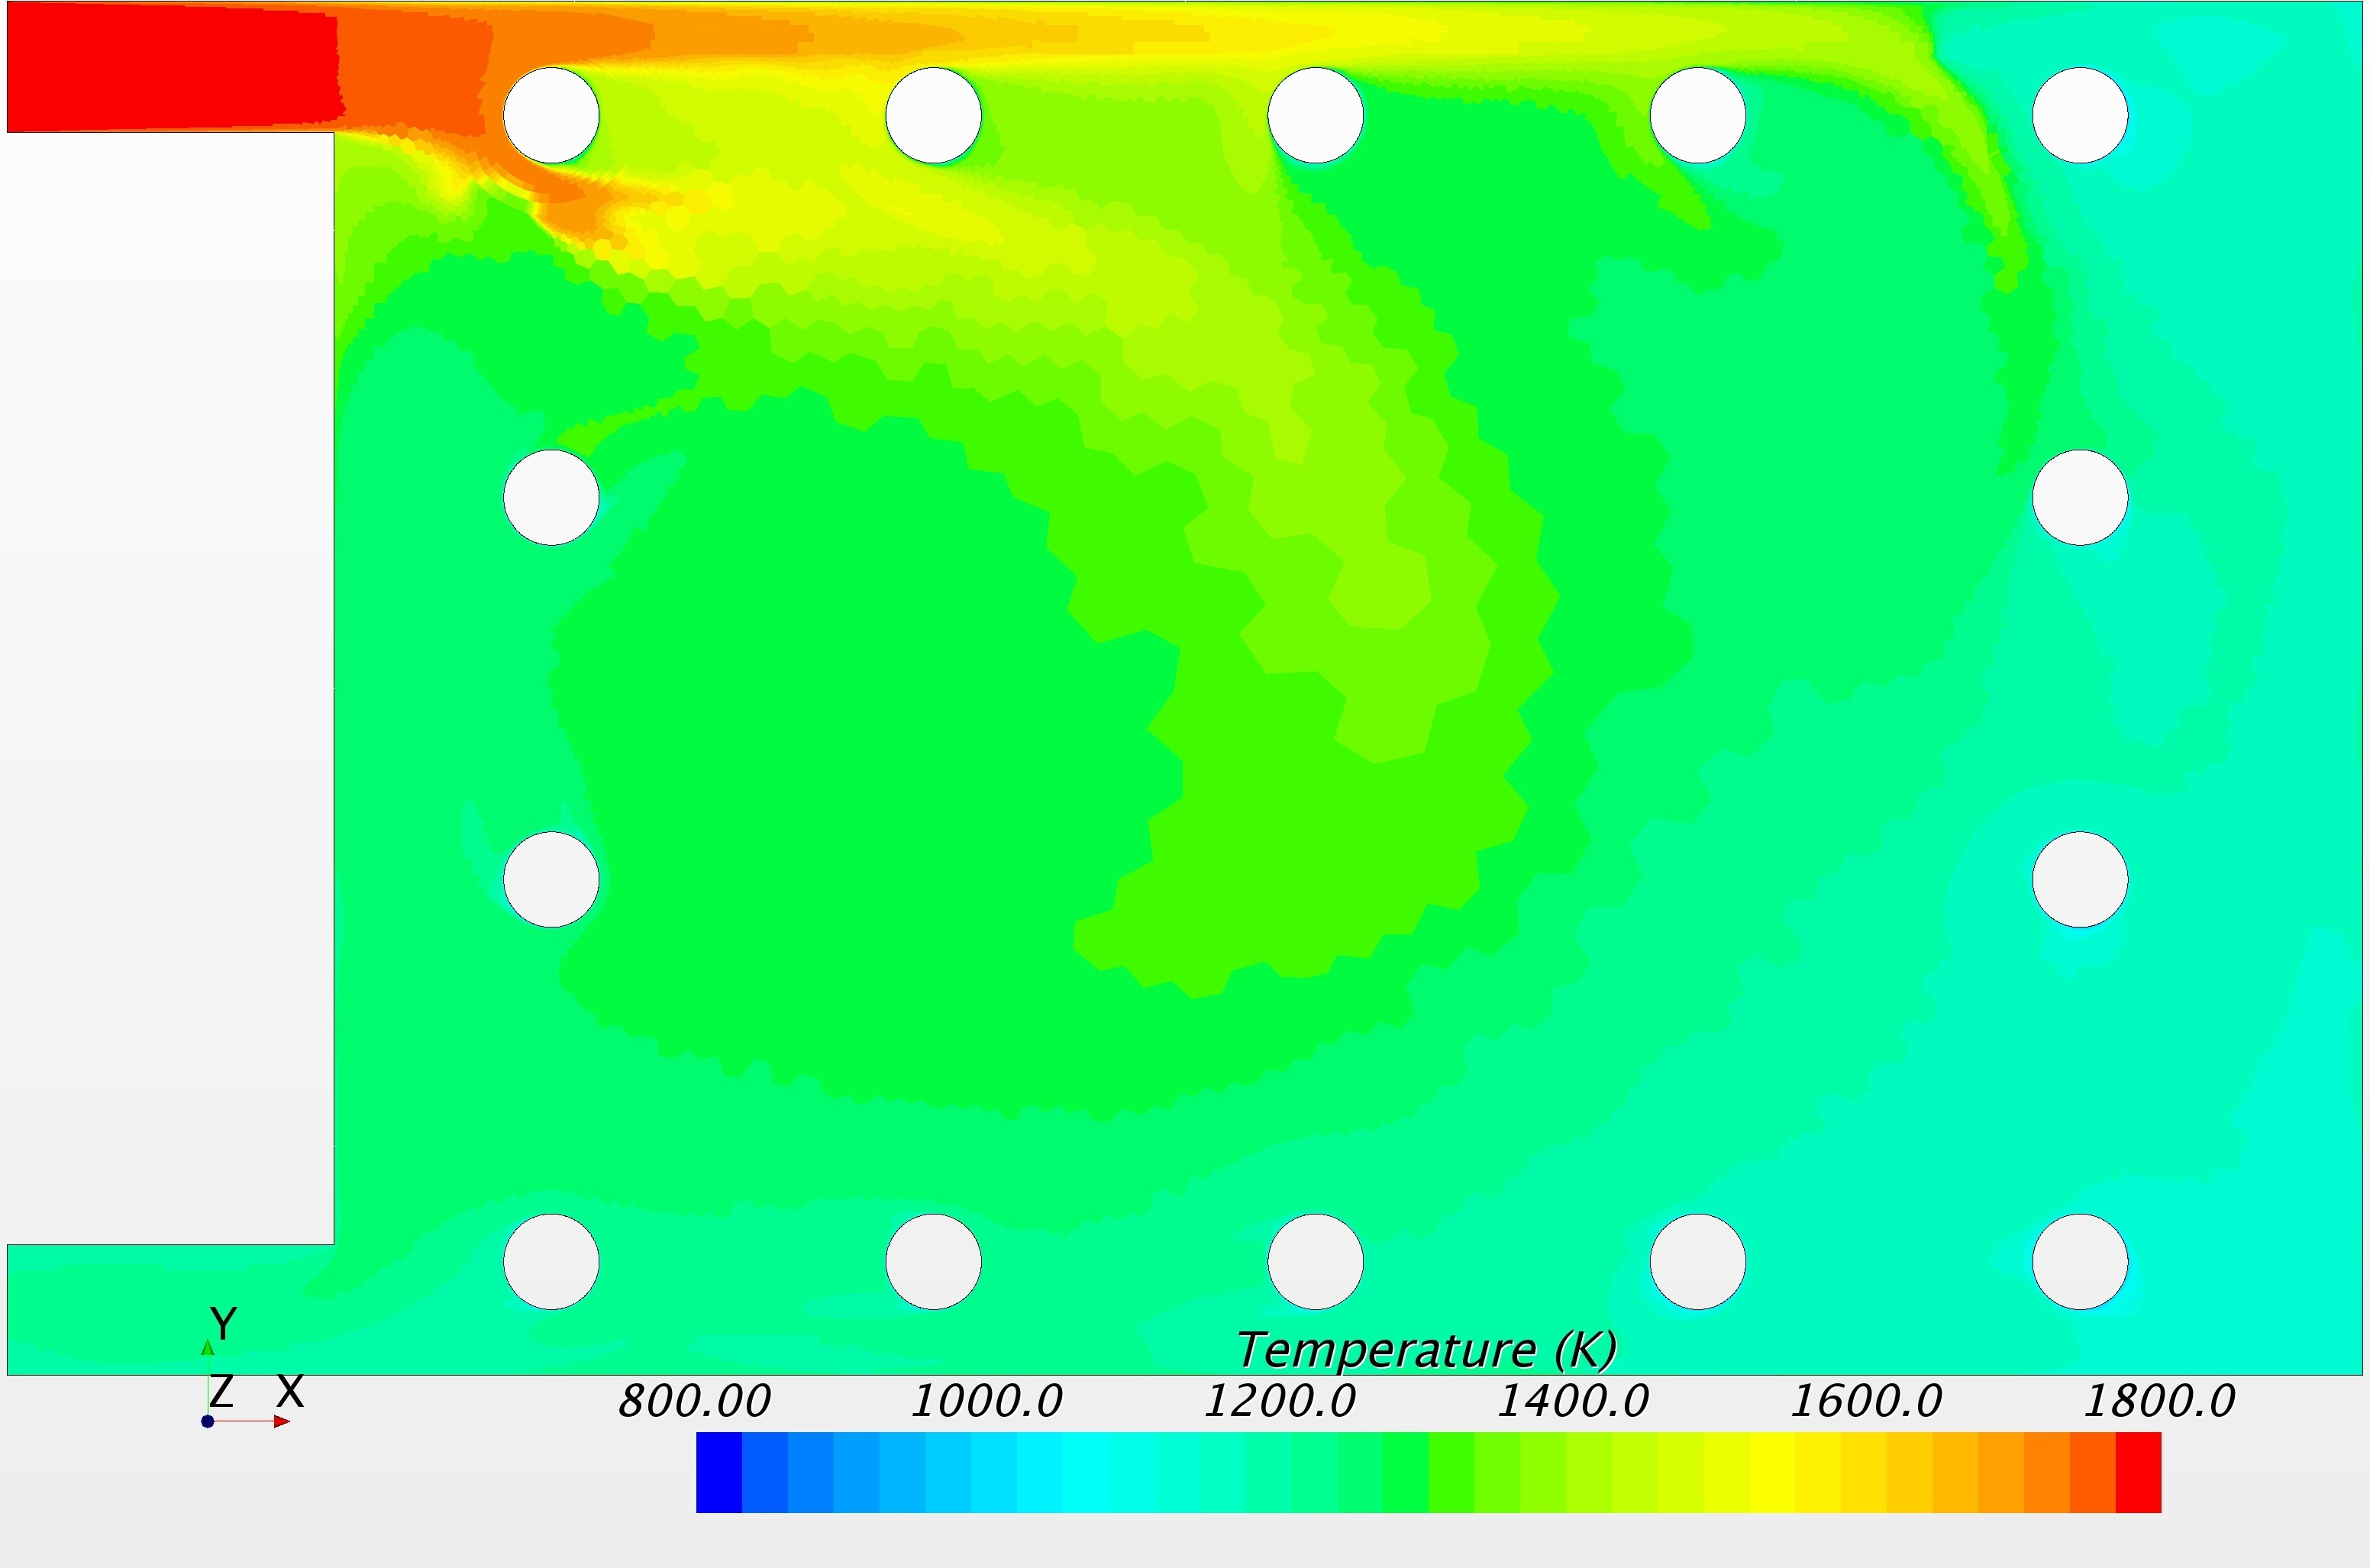
\includegraphics[height=3.8cm]{sources/figure8/c-temp_11.jpg}};
% \node (n12b) [right=0.05cm of n12a] {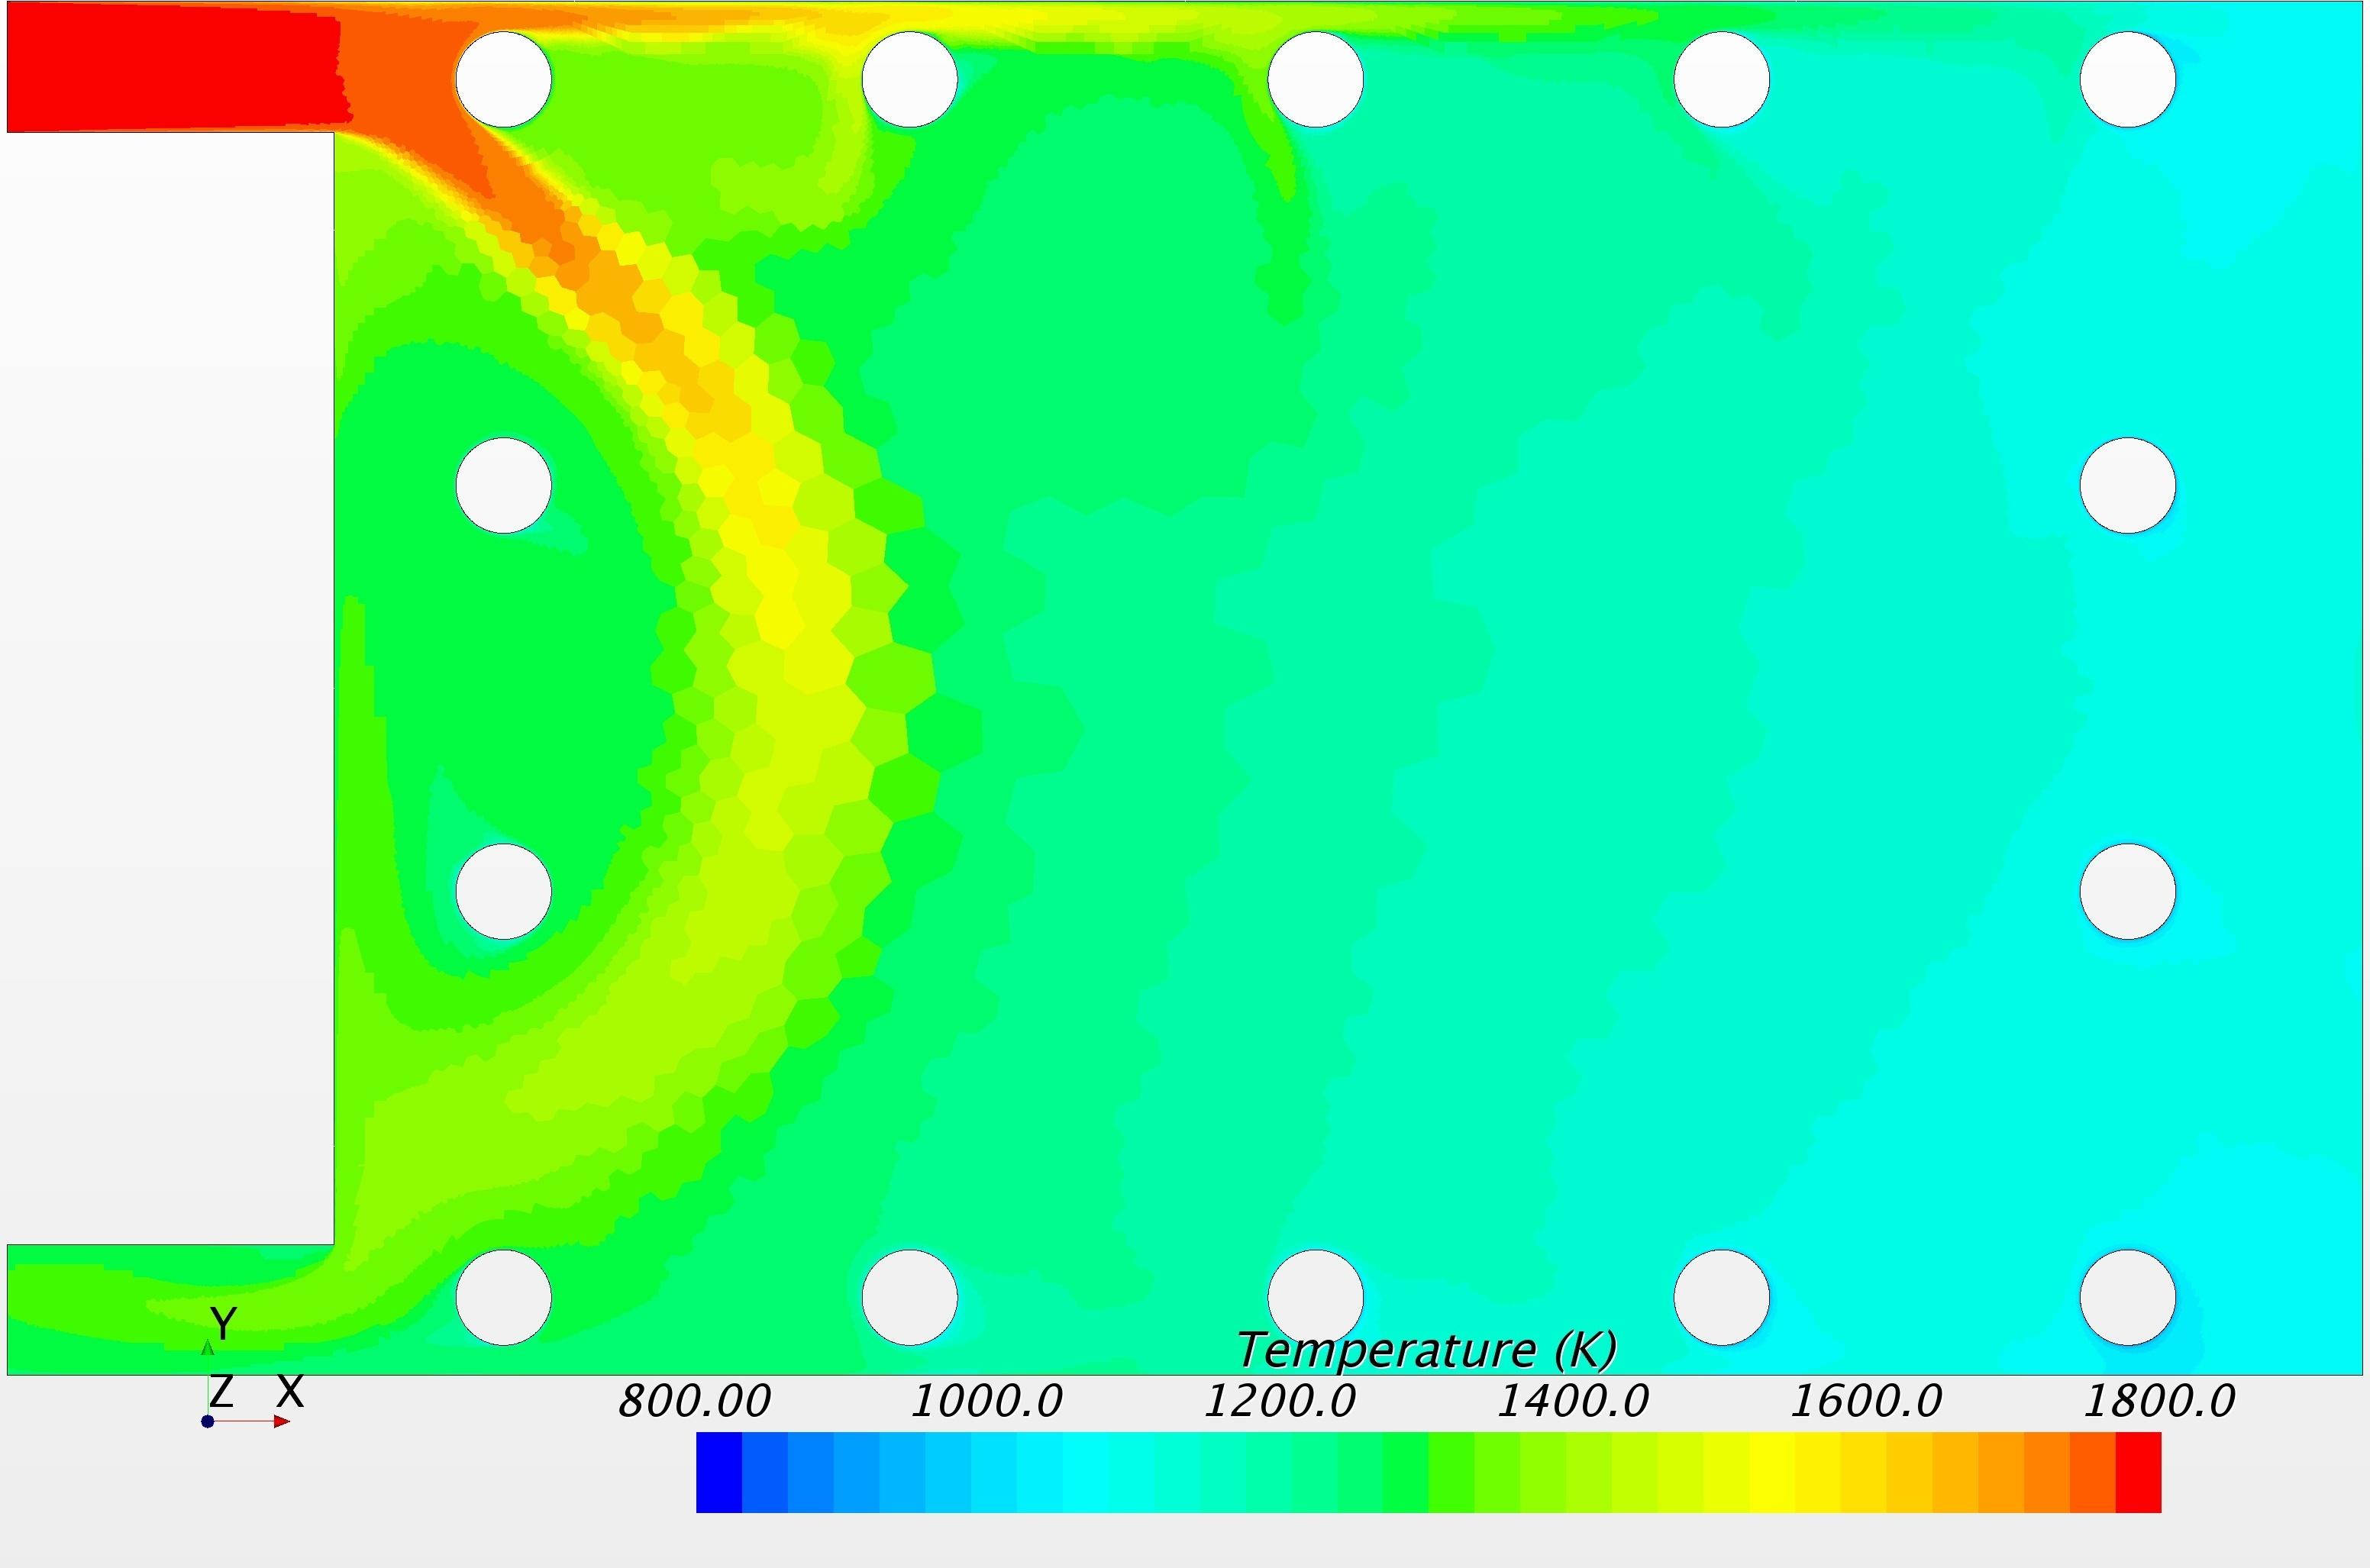
\includegraphics[height=3.8cm]{sources/figure8/c-temp_12.jpg}};



\node (n1c) [right=0.25cm of n1b,align=left] {\renewcommand\arraystretch{0.8}\setlength{\tabcolsep}{1pt}{\scalebox{1.0}{\begin{tabular}{ll}\gls{distancefactor}&$=1.25$ \\ $\gls{heatfluxratio}$&$=95.24\%$ \\ $\gls{heatfluxmean}$&$=11870\si{\watt}$ \\ $\gls{viewfactormean}$&$=0.52$ \\ \end{tabular}}}};
% \node (n2c) [right=0.25cm of n2b,align=left] {\renewcommand\arraystretch{0.8}\setlength{\tabcolsep}{1pt}{\scalebox{1.0}{\begin{tabular}{ll}\gls{distancefactor}&$=1.50$ \\ $\gls{heatfluxratio}$&$=95.60\%$ \\ $\gls{heatfluxmean}$&$=13233\si{\watt}$ \\ $\gls{viewfactormean}$&$=0.46$ \\ \end{tabular}}}};
\node (n3c) [right=0.25cm of n3b,align=left] {\renewcommand\arraystretch{0.8}\setlength{\tabcolsep}{1pt}{\scalebox{1.0}{\begin{tabular}{ll}\gls{distancefactor}&$=1.75$ \\ $\gls{heatfluxratio}$&$=95.78\%$ \\ $\gls{heatfluxmean}$&$=14166\si{\watt}$ \\ $\gls{viewfactormean}$&$=0.41$ \\ \end{tabular}}}};
% \node (n4c) [right=0.25cm of n4b,align=left] {\renewcommand\arraystretch{0.8}\setlength{\tabcolsep}{1pt}{\scalebox{1.0}{\begin{tabular}{ll}\gls{distancefactor}&$=2.00$ \\ $\gls{heatfluxratio}$&$=95.61\%$ \\ $\gls{heatfluxmean}$&$=15006\si{\watt}$ \\ $\gls{viewfactormean}$&$=0.37$ \\ \end{tabular}}}};
\node (n5c) [right=0.25cm of n5b,align=left] {\renewcommand\arraystretch{0.8}\setlength{\tabcolsep}{1pt}{\scalebox{1.0}{\begin{tabular}{ll}\gls{distancefactor}&$=2.25$ \\ $\gls{heatfluxratio}$&$=95.47\%$ \\ $\gls{heatfluxmean}$&$=15711\si{\watt}$ \\ $\gls{viewfactormean}$&$=0.33$ \\ \end{tabular}}}};
% \node (n6c) [right=0.25cm of n6b,align=left] {\renewcommand\arraystretch{0.8}\setlength{\tabcolsep}{1pt}{\scalebox{1.0}{\begin{tabular}{ll}\gls{distancefactor}&$=2.375$ \\ $\gls{heatfluxratio}$&$=95.23\%$ \\ $\gls{heatfluxmean}$&$=16018\si{\watt}$ \\ $\gls{viewfactormean}$&$=0.31$ \\ \end{tabular}}}};
\node (n7c) [right=0.25cm of n7b,align=left] {\renewcommand\arraystretch{0.8}\setlength{\tabcolsep}{1pt}{\scalebox{1.0}{\begin{tabular}{ll}\gls{distancefactor}&$=2.50$ \\ $\gls{heatfluxratio}$&$=94.69\%$ \\ $\gls{heatfluxmean}$&$=16200\si{\watt}$ \\ $\gls{viewfactormean}$&$=0.30$ \\ \end{tabular}}}};
% \node (n8c) [right=0.25cm of n8b,align=left] {\renewcommand\arraystretch{0.8}\setlength{\tabcolsep}{1pt}{\scalebox{1.0}{\begin{tabular}{ll}\gls{distancefactor}&$=2.75$ \\ $\gls{heatfluxratio}$&$=93.31\%$ \\ $\gls{heatfluxmean}$&$=16718\si{\watt}$ \\ $\gls{viewfactormean}$&$=0.27$ \\ \end{tabular}}}};
% \node (n9c) [right=0.25cm of n9b,align=left] {\renewcommand\arraystretch{0.8}\setlength{\tabcolsep}{1pt}{\scalebox{1.0}{\begin{tabular}{ll}\gls{distancefactor}&$=3.00$ \\ $\gls{heatfluxratio}$&$=92.89\%$ \\ $\gls{heatfluxmean}$&$=17118\si{\watt}$ \\ $\gls{viewfactormean}$&$=0.25$ \\ \end{tabular}}}};
\node (n10c) [right=0.25cm of n10b,align=left] {\renewcommand\arraystretch{0.8}\setlength{\tabcolsep}{1pt}{\scalebox{1.0}{\begin{tabular}{ll}\gls{distancefactor}&$=3.50$ \\ $\gls{heatfluxratio}$&$=91.88\%$ \\ $\gls{heatfluxmean}$&$=17319\si{\watt}$ \\ $\gls{viewfactormean}$&$=0.22$ \\ \end{tabular}}}};
\node (n11c) [right=0.25cm of n11b,align=left] {\renewcommand\arraystretch{0.8}\setlength{\tabcolsep}{1pt}{\scalebox{1.0}{\begin{tabular}{ll}\gls{distancefactor}&$=4.00$ \\ $\gls{heatfluxratio}$&$=91.92\%$ \\ $\gls{heatfluxmean}$&$=17920\si{\watt}$ \\ $\gls{viewfactormean}$&$=0.19$ \\ \end{tabular}}}};
% \node (n12c) [right=0.25cm of n12b,align=left] {\renewcommand\arraystretch{0.8}\setlength{\tabcolsep}{1pt}{\scalebox{1.0}{\begin{tabular}{ll}\gls{distancefactor}&$=4.25$ \\ $\gls{heatfluxratio}$&$=91.31\%$ \\ $\gls{heatfluxmean}$&$=15506\si{\watt}$ \\ $\gls{viewfactormean}$&$=0.18$ \\ \end{tabular}}}};

\end{tikzpicture}

%	\caption{
%		Velocity magnitude (left column) and temperature fields (right column) for the configuration \gls{caseD} at different distance factors with an inner tube radius of $\gls{radius}=\SI{0.063}{\meter}$, and a flue gas mass flow of $\gls{massflow}=\SI{0.03}{\kilogram\per\second\per{tube}}$.
%	}%
%	\label{f:matrix}
\end{figure}
\efloatseparator
%%
\textwidth=85mm
\begin{figure}
	\centering
	
\usetikzlibrary{plotmarks,fit}
\begin{tikzpicture}
%\pgfplotsset{set layers=default};
\begin{axis}[
		width=80mm,
		height=60mm,     % size of the image
		grid = major,
		grid style={line width=.1pt, draw=gray!10},
		xmin=4000,     % start the diagram at this x-coordinate
		xmax=28000,    % end   the diagram at this x-coordinate
		ymin=0,     % start the diagram at this y-coordinate
		ymax=0.7,   % end   the diagram at this y-coordinate
		axis background/.style={fill=white},
		xlabel={\gls{heatfluxmean} / \si{\watt}},
		ylabel={\gls{viewfactormean} / --},
		ylabel style={align=center},
		tick align=inside,
		cycle list name=mpiovgucolors2d,
		scaled x ticks=true,
		every x tick label/.append style={alias=XTick,inner xsep=0pt},
		every x tick scale label/.style={at=(XTick.base east),anchor=base west},
		% change `clip mode' to `individual' to avoid unwanted clipping
		clip mode=individual,
	]

	%% import the correct data from a CSV file
	\addplot+[scatter=true,only marks, on layer=leins,point meta=explicit symbolic,scatter/@pre marker code/.style={/tikz/mark size=sqrt(\pgfplotspointmeta/\PI)*25}, scatter/@post marker code/.style={}]  table[x=HeatTransferMean(W),y=Approximated View Factor Per Tube (-),meta=MassFlowPerTube (kg/s),col sep=semicolon] {sources/figure9/resultsCaseA-0.04.csv};
		\label{p:vfvmhf_a4}
	\addplot+[scatter=true,only marks, on layer=leins,point meta=explicit symbolic,scatter/@pre marker code/.style={/tikz/mark size=sqrt(\pgfplotspointmeta/\PI)*25}, scatter/@post marker code/.style={}]  table[x=HeatTransferMean(W),y=Approximated View Factor Per Tube (-),meta=MassFlowPerTube (kg/s),col sep=semicolon] {sources/figure9/resultsCaseA-0.063.csv};
		\label{p:vfvmhf_a6}
	\addplot+[scatter=true,only marks, on layer=leins,point meta=explicit symbolic,scatter/@pre marker code/.style={/tikz/mark size=sqrt(\pgfplotspointmeta/\PI)*25}, scatter/@post marker code/.style={}]  table[x=HeatTransferMean(W),y=Approximated View Factor Per Tube (-),meta=MassFlowPerTube (kg/s),col sep=semicolon] {sources/figure9/resultsCaseA-0.08.csv};
		\label{p:vfvmhf_a8}
	\addplot+[scatter=true,only marks, on layer=lzwei,point meta=explicit symbolic,scatter/@pre marker code/.style={/tikz/mark size=sqrt(\pgfplotspointmeta/\PI)*25}, scatter/@post marker code/.style={}]  table[x=HeatTransferMean(W),y=Approximated View Factor Per Tube (-),meta=MassFlowPerTube (kg/s),col sep=semicolon] {sources/figure9/resultsCaseB-0.04.csv};
		\label{p:vfvmhf_b4}
	\addplot+[scatter=true,only marks, on layer=lzwei,point meta=explicit symbolic,scatter/@pre marker code/.style={/tikz/mark size=sqrt(\pgfplotspointmeta/\PI)*25}, scatter/@post marker code/.style={}]  table[x=HeatTransferMean(W),y=Approximated View Factor Per Tube (-),meta=MassFlowPerTube (kg/s),col sep=semicolon] {sources/figure9/resultsCaseB-0.063.csv};
		\label{p:vfvmhf_b6}
	\addplot+[scatter=true,only marks, on layer=lzwei,point meta=explicit symbolic,scatter/@pre marker code/.style={/tikz/mark size=sqrt(\pgfplotspointmeta/\PI)*25}, scatter/@post marker code/.style={}]  table[x=HeatTransferMean(W),y=Approximated View Factor Per Tube (-),meta=MassFlowPerTube (kg/s),col sep=semicolon] {sources/figure9/resultsCaseB-0.08.csv};
		\label{p:vfvmhf_b8}
	\addplot+[scatter=true,only marks, on layer=ldrei,point meta=explicit symbolic,scatter/@pre marker code/.style={/tikz/mark size=sqrt(\pgfplotspointmeta/\PI)*25}, scatter/@post marker code/.style={}]  table[x=HeatTransferMean(W),y=Approximated View Factor Per Tube (-),meta=MassFlowPerTube (kg/s),col sep=semicolon] {sources/figure9/resultsCaseC-0.04.csv};
		\label{p:vfvmhf_c4}
	\addplot+[scatter=true,only marks, on layer=ldrei,point meta=explicit symbolic,scatter/@pre marker code/.style={/tikz/mark size=sqrt(\pgfplotspointmeta/\PI)*25}, scatter/@post marker code/.style={}]  table[x=HeatTransferMean(W),y=Approximated View Factor Per Tube (-),meta=MassFlowPerTube (kg/s),col sep=semicolon] {sources/figure9/resultsCaseC-0.063.csv};
		\label{p:vfvmhf_c6}
	\addplot+[scatter=true,only marks, on layer=ldrei,point meta=explicit symbolic,scatter/@pre marker code/.style={/tikz/mark size=sqrt(\pgfplotspointmeta/\PI)*25}, scatter/@post marker code/.style={}]  table[x=HeatTransferMean(W),y=Approximated View Factor Per Tube (-),meta=MassFlowPerTube (kg/s),col sep=semicolon] {sources/figure9/resultsCaseC-0.08.csv};
		\label{p:vfvmhf_c8}
	\addplot+[scatter=true,only marks, on layer=lvier,point meta=explicit symbolic,scatter/@pre marker code/.style={/tikz/mark size=sqrt(\pgfplotspointmeta/\PI)*25}, scatter/@post marker code/.style={}]  table[x=HeatTransferMean(W),y=Approximated View Factor Per Tube (-),meta=MassFlowPerTube (kg/s),col sep=semicolon] {sources/figure9/resultsCaseD-0.04.csv};
		\label{p:vfvmhf_d4}
	\addplot+[scatter=true,only marks, on layer=lvier,point meta=explicit symbolic,scatter/@pre marker code/.style={/tikz/mark size=sqrt(\pgfplotspointmeta/\PI)*25}, scatter/@post marker code/.style={}]  table[x=HeatTransferMean(W),y=Approximated View Factor Per Tube (-),meta=MassFlowPerTube (kg/s),col sep=semicolon] {sources/figure9/resultsCaseD-0.063.csv};
		\label{p:vfvmhf_d6}
	\addplot+[scatter=true,only marks, on layer=lvier,point meta=explicit symbolic,scatter/@pre marker code/.style={/tikz/mark size=sqrt(\pgfplotspointmeta/\PI)*25}, scatter/@post marker code/.style={}]  table[x=HeatTransferMean(W),y=Approximated View Factor Per Tube (-),meta=MassFlowPerTube (kg/s),col sep=semicolon] {sources/figure9/resultsCaseD-0.08.csv};
		\label{p:vfvmhf_d8}

	\coordinate (xcenter) at (axis description cs:0.5,0);
\end{axis};

%% Multi legend
\node[
below,
rectangle,
draw=black, thin,
inner sep=1pt,
] at (xcenter |- current bounding box.south) {
	\tikz{
		\node (L1) {
			\renewcommand\arraystretch{0.8}\setlength{\tabcolsep}{3pt}
			\begin{tabular}{rccc}
				\rotatebox{90}{~\rotatebox{-90}{\scriptsize \gls{radius} / \si{\meter}}}& \rotatebox{90}{\scriptsize 0.04} & \rotatebox{90}{\scriptsize 0.063} & \rotatebox{90}{\scriptsize 0.08} \\
			\scriptsize  line 		& \ref*{p:vfvmhf_a4} 	& \ref*{p:vfvmhf_a6} 	& \ref*{p:vfvmhf_a8} \\
			\scriptsize staggered 	& \ref*{p:vfvmhf_b4} 	& \ref*{p:vfvmhf_b6} 	& \ref*{p:vfvmhf_b8} \\
			\scriptsize aligned 		& \ref*{p:vfvmhf_c4} 	& \ref*{p:vfvmhf_c6} 	& \ref*{p:vfvmhf_c8} \\
			\scriptsize rectangle 	& \ref*{p:vfvmhf_d4} 	& \ref*{p:vfvmhf_d6} 	& \ref*{p:vfvmhf_d8} \\
			\end{tabular}
		};
		\node[right of=L1,xshift=1cm,anchor=west] {
			\tikz[]{
				\draw(0,0)--(0,1.5);
				\foreach \y/\ytext in {0/~,0.25/0.01,0.50/~,0.75/0.02,1.00/~,1.25/0.03,1.50/~}
				\draw(-2pt,\y)--(2pt,\y) node[right] {\tiny\ytext};
				
				\foreach \y/\ytext in {0/1.00pt,.25/1.41pt,.50/1.73pt,.75/1.99pt,1.00/2.23pt,1.25/2.44pt,1.50/2.64pt}
				\draw[black!40] (-6pt,\y) circle (\ytext);
				
				\node[anchor=south,rotate=90,inner sep=0pt] at (-15pt,0.75) {\scriptsize\gls{massflow} / \si{\kilogram\per\second\per{tube}}}
			}
		};
	}
};

\end{tikzpicture}

%	\caption{
%		Average view factor \gls{viewfactormean} versus mean heat flux \gls{heatfluxmean}.
%		The symbol (and its color family) indicates the configuration of the data point.
%		Shades of the respective color indicate the inner tube radius~\gls{radius}.
%		Symbol size indicates the mass flow rate~\gls{massflow} of flue gas per reforming tube.
%	}%
%	\label{f:viewfactor2meanheatflux}
\end{figure}
\efloatseparator
%%

\begin{figure}
	\centering
	\begin{tikzpicture}
	\begin{axis}[
			width=16.5pc, 
			height=15pc,     % size of the image
			grid = major,
			grid style={line width=.1pt, draw=gray!10},	     	
			xmin=1.2,     % start the diagram at this x-coordinate
			xmax=4.3,    % end   the diagram at this x-coordinate	    
			ymin=900,     % start the diagram at this y-coordinate
			ymax=1100,   % end   the diagram at this y-coordinate
			axis background/.style={fill=white},
			xlabel={\gls{distancefactor} / --},
			ylabel={\gls{tempmean} / \si{\kelvin}},
			ylabel style={align=center},
			tick align=inside,
			minor y tick num=3,
			minor x tick num=3,
			% change `clip mode' to `individual' to avoid unwanted clipping
			%clip mode=individual,
			]

			%% import the correct data from a CSV file
			\addplot+[only marks, on layer=lzwei, scatter=true, point meta=explicit symbolic,scatter/@pre marker code/.style={/tikz/mark size=sqrt(\pgfplotspointmeta/\PI)*25}, scatter/@post marker code/.style={}, mpiblue, 	every mark/.append style={solid}, mark=otimes]  table[col sep=semicolon,x=DistanceFactor,y=MeanTubeTemps(K), meta=MassFlowPerTube (kg/s)] {sources/figure10/resultsCaseB-0.063.csv};
			\label{p:dvmtb6}
			\addplot+[only marks, on layer=ldrei, scatter=true, point meta=explicit symbolic,scatter/@pre marker code/.style={/tikz/mark size=sqrt(\pgfplotspointmeta/\PI)*25}, scatter/@post marker code/.style={},vstred100, 	every mark/.append style={solid}, mark=triangle]  table[col sep=semicolon,x=DistanceFactor,y=MeanTubeTemps(K), meta=MassFlowPerTube (kg/s)] {sources/figure10/resultsCaseC-0.063.csv};
			\label{p:dvmtc6}
			\addplot+[only marks, on layer=leins, black, every mark/.append style={solid}, mark=otimes, mark size=1.41pt] table[col sep=semicolon,x=DistanceFactor, y=MeanTemperature,] {sources/rad_model_aligned.csv};
			\label{p:dvmt_mb}
			\addplot+[only marks, on layer=leins, black, every mark/.append style={solid}, mark=triangle, mark size=1.41pt] table[col sep=semicolon,x=DistanceFactor, y=MeanTemperature,] {sources/rad_model_staggered.csv};
			\label{p:dvmt_mc}


			\coordinate (xcenter) at (axis description cs:0.5,0.98); 
			
			\node [anchor=east]at (rel axis cs:1,0.08) {\scalebox{.6}{$0.005$}};
			\node [anchor=east]at (rel axis cs:1,0.35) {\scalebox{.6}{$0.010$}};
			\node [anchor=east]at (rel axis cs:1,0.63) {\scalebox{.6}{$0.015$}};
	\end{axis};
	% Multi legend
	\node[
		below,
		rectangle,
		draw=black, thin,
		fill=white,
		inner sep=1pt,
	%] at (xcenter |- current bounding box.south) {
		anchor=north,
	] at (xcenter) {
		\tikz{
			\node (L1) {
				\renewcommand\arraystretch{0.5}\setlength{\tabcolsep}{3pt}
				\begin{tabular}{rcc}
					& \scalebox{.6}{CFD} & \scalebox{.6}{Liesche (2019)} \\
					\scalebox{.6}{staggered} 	& \ref*{p:dvmtb6} & \ref*{p:dvmt_mb} \\
					\scalebox{.6}{aligned} 		& \ref*{p:dvmtc6} & \ref*{p:dvmt_mc}\\
				\end{tabular}
				};
				\node[right of=L1,xshift=2pc,anchor=west] {
					\tikz[]{
						\draw(0,0)--(1,0);
						\foreach \x/\xtext in {0/0.005,0.5/0.010,1/0.015}
						\draw(\x,2pt)--(\x,-2pt) node[below,anchor=north] {\scalebox{.4}{\xtext}};

						\foreach \x/\xtext in {0/1.00pt,.5/1.41pt,1/1.73pt}
						\draw[black!40] (\x,6pt) circle (\xtext);

						\node[anchor=south,inner sep=0pt] at (0.5,10pt) {\scalebox{.6}{\gls{massflow} / \si{\kilogram\per\second\per{tube}}}};
					}
				};
			}
		};


\end{tikzpicture}

%	\caption{
%		Mean tube surface temperature of all tubes in the bundle \gls{tempmean} versus distance factor \gls{distancefactor} for staggered and aligned arrangements.
%		Results from the radiation-based model~\citep{Liesche.2019b} are marked with black symbols of the respective staggered and aligned arrangements.
%	}%
%	\label{f:T_sta_vs_ali}
\end{figure}
\efloatseparator
%%

\textwidth=180mm
\begin{figure}
	\centering
	\begin{tikzpicture}
	\begin{axis}[
			name=plot1,
			width=45mm,
			height=45mm,     % size of the image
			scale only axis=true,
			grid = major,
			grid style={line width=.1pt, draw=gray!10},	     	
			xmin=1.8,     % start the diagram at this x-coordinate
			xmax=6.3,    % end   the diagram at this x-coordinate	    
			ymin=900,     % start the diagram at this y-coordinate
			ymax=1150,   % end   the diagram at this y-coordinate
			axis background/.style={fill=white},
			xlabel={\gls{distancefactor} / --},
			ylabel={\gls{tempmean} / \si{\kelvin}},
			ylabel style={align=center},
			tick align=inside,
			minor y tick num=1,
			minor x tick num=1,
			% change `clip mode' to `individual' to avoid unwanted clipping
			clip mode=individual,
			]

			%% import the correct data from a CSV file
			\addplot+[scatter=true, point meta=explicit symbolic,scatter/@pre marker code/.style={/tikz/mark size=sqrt(\pgfplotspointmeta/\PI)*25}, scatter/@post marker code/.style={},mpiblue150, every mark/.append style={solid}, mark=otimes, error bars/.cd, y dir=both, y explicit,]  table[col sep=semicolon,x=DistanceFactor,y=MeanTubeTemps(K), meta=MassFlowPerTube (kg/s), y error=stdTubeTemps(K)] {sources/figure11/resultsCaseB-0.04.csv};
			\label{p:teb_b4};
			\addplot+[black, every mark/.append style={solid}, mark=otimes, mark size=1.41pt, error bars/.cd, y dir=both, y explicit, ] table[col sep=comma,x=distanceFactor, y=meanTemp,y error=meanTempSD] {sources/figure11/rad_results_staggered_040_transposed.csv};
	\end{axis};
	\begin{axis}[
			name=plot2,
			at={($(plot1.south east)+(1pc,0)$)},
			anchor=south west,
			width=45mm,
			height=45mm,     % size of the image
			scale only axis=true,
			grid = major,
			grid style={line width=.1pt, draw=gray!10},	     	
			xmin=1.2,     % start the diagram at this x-coordinate
			xmax=4.3,    % end   the diagram at this x-coordinate	    
			ymin=900,     % start the diagram at this y-coordinate
			ymax=1050,   % end   the diagram at this y-coordinate
			axis background/.style={fill=white},
			xlabel={\gls{distancefactor} / --},
			tick align=inside,
			minor y tick num=1,
			minor x tick num=1,
%			ylabel={\gls{tempmean} / \si{\kelvin}},
%			ylabel style={align=center},
			yticklabels=\empty,
			% change `clip mode' to `individual' to avoid unwanted clipping
			clip mode=individual,
			]

			%% import the correct data from a CSV file
			\addplot+[scatter=true, point meta=explicit symbolic,scatter/@pre marker code/.style={/tikz/mark size=sqrt(\pgfplotspointmeta/\PI)*25}, scatter/@post marker code/.style={},mpiblue, every mark/.append style={solid}, mark=otimes, error bars/.cd, y dir=both, y explicit,]  table[col sep=semicolon,x=DistanceFactor,y=MeanTubeTemps(K), meta=MassFlowPerTube (kg/s), y error=stdTubeTemps(K)] {sources/figure11/resultsCaseB-0.063.csv};
			\label{p:teb_b6};
			\addplot+[black, every mark/.append style={solid}, mark=otimes, mark size=1.41pt, error bars/.cd, y dir=both, y explicit, ] table[col sep=comma,x=distanceFactor, y=meanTemp,y error=meanTempSD] {sources/figure11/rad_results_staggered_063_transposed.csv};
				\label{p:teb_ref};
	\end{axis};
	\begin{axis}[
			name=plot3,
			at={($(plot2.south east)+(1pc,0)$)},
			anchor=south west,
			width=45mm,
			height=45mm,     % size of the image
			scale only axis=true,
			grid = major,
			grid style={line width=.1pt, draw=gray!10},	     	
			xmin=1,     % start the diagram at this x-coordinate
			xmax=3.5,    % end   the diagram at this x-coordinate	    
			ymin=900,     % start the diagram at this y-coordinate
			ymax=1150,   % end   the diagram at this y-coordinate
			axis background/.style={fill=white},
			xlabel={\gls{distancefactor} / --},
			tick align=inside,
			minor y tick num=1,
			minor x tick num=1,
			yticklabels=\empty,
			% change `clip mode' to `individual' to avoid unwanted clipping
			clip mode=individual,
			]

			%% import the correct data from a CSV file
			\addplot+[scatter=true, point meta=explicit symbolic,scatter/@pre marker code/.style={/tikz/mark size=sqrt(\pgfplotspointmeta/\PI)*25}, scatter/@post marker code/.style={},mpiblue050, every mark/.append style={solid}, mark=otimes, error bars/.cd, y dir=both, y explicit,]  table[col sep=semicolon,x=DistanceFactor,y=MeanTubeTemps(K), meta=MassFlowPerTube (kg/s), y error=stdTubeTemps(K)] {sources/figure11/resultsCaseB-0.08.csv};
			\label{p:teb_b8};
			\addplot+[black, every mark/.append style={solid}, mark=otimes, mark size=1.41pt, error bars/.cd, y dir=both, y explicit, ] table[col sep=comma,x=distanceFactor, y=meanTemp,y error=meanTempSD] {sources/figure11/rad_results_staggered_080_transposed.csv};
%			\label{p:teb_ref};

			\coordinate (c3) at (rel axis cs:1,1);

\node[
	rectangle,
	draw=black, thin,
	fill=white,
	anchor= north east,
	inner sep=1pt,
	on layer=foreground,
	] at (c3) {
	\tikz[node distance=0.1cm]{
		\node (L1) [inner sep=3pt] {
			\renewcommand\arraystretch{0.5}\setlength{\tabcolsep}{2pt}
			\begin{tabular}{rccc}
				\scalebox{.6}{\gls{radius} / \si{\meter}}& \scalebox{.6}{0.04} & \scalebox{.6}{0.063} & \scalebox{.6}{0.08} \\
				\scalebox{.6}{staggered}	& \ref*{p:teb_b4} 	& \ref*{p:teb_b6} 	& \ref*{p:teb_b8}  \\
			\end{tabular}
		};
	
		\node (L2) [below=0pc and 4pc of L1, anchor=north,inner sep=3pt] {
			\renewcommand\arraystretch{0.5}\setlength{\tabcolsep}{2pt}
			\begin{tabular}{rc}
				\scalebox{.6}{ Liesche (2019)} & \ref{p:teb_ref} \\
			\end{tabular}
		}
	}
};

	\end{axis};

\end{tikzpicture}
%
%	\caption{
%		Mean tube surface temperature \gls{tempmean} versus distance factor \gls{distancefactor} for staggered arrangements (\gls{caseB}) based on the radiation model (black) and CFD model (blue) for three different tube radii.
%		Error bars show the standard deviation of the respective data set.
%	}%
%	\label{f:rad_vs_CFD_2}
\end{figure}
\efloatseparator
%%

\textwidth=85mm
\begin{figure}
	\centering
	
\usetikzlibrary{plotmarks}
\begin{tikzpicture}
\begin{axis}[
			width=75mm,
			height=80mm,     % size of the image
			grid = major,
			grid style={line width=.1pt, draw=gray!10},
			xmin=4000,     % start the diagram at this x-coordinate
			xmax=27000,    % end   the diagram at this x-coordinate
			ymin=650,     % start the diagram at this y-coordinate
			ymax=1400,   % end   the diagram at this y-coordinate
			axis background/.style={fill=white},
			xlabel={\gls{heatfluxmean} / \si{\watt}},
			ylabel={\gls{tempmean} / \si{\kelvin}},
			ylabel style={align=center},
			tick align=inside,
			minor y tick num=3,
			minor x tick num=1,
			cycle list name=mpiovgucolors2d,
%			scaled x ticks=true,
%			every x tick label/.append style={alias=XTick,inner xsep=0pt},
%			every x tick scale label/.style={at=(XTick.base east),anchor=base west},
			% change `clip mode' to `individual' to avoid unwanted clipping
			clip mode=individual,
		]

	%% import the correct data from a CSV file
	\addplot+[only marks, on layer=leins, error bars/.cd, y dir=both, y explicit, error bar style={line width=0.25pt,opacity=1.0,},error mark options={line width=0.25pt,opacity=1.0,}]  table[x=HeatTransferMean(W),y=MeanTubeTemps(K), y error minus expr={\thisrow{MeanTubeTemps(K)}-\thisrow{MinTubeTemp(K)}}, y error plus expr={\thisrow{MaxTubeTemp(K)}-\thisrow{MeanTubeTemps(K)}}, col sep=semicolon] {sources/figure12/resultsCaseA-0.04.csv};
		\label{p:tempa4}
	\addplot+[only marks, on layer=leins, error bars/.cd, y dir=both, y explicit, error bar style={line width=0.25pt,opacity=1.0,},error mark options={line width=0.25pt,opacity=1.0,}]  table[x=HeatTransferMean(W),y=MeanTubeTemps(K), y error minus expr={\thisrow{MeanTubeTemps(K)}-\thisrow{MinTubeTemp(K)}}, y error plus expr={\thisrow{MaxTubeTemp(K)}-\thisrow{MeanTubeTemps(K)}}, col sep=semicolon] {sources/figure12/resultsCaseA-0.063.csv};
		\label{p:tempa6}
	\addplot+[only marks, on layer=leins, error bars/.cd, y dir=both, y explicit, error bar style={line width=0.25pt,opacity=1.0,},error mark options={line width=0.25pt,opacity=1.0,}]  table[x=HeatTransferMean(W),y=MeanTubeTemps(K), y error minus expr={\thisrow{MeanTubeTemps(K)}-\thisrow{MinTubeTemp(K)}}, y error plus expr={\thisrow{MaxTubeTemp(K)}-\thisrow{MeanTubeTemps(K)}}, col sep=semicolon] {sources/figure12/resultsCaseA-0.08.csv};
		\label{p:tempa8}
	\addplot+[only marks, on layer=lzwei, error bars/.cd, y dir=both, y explicit, error bar style={line width=0.25pt,opacity=1.0,},error mark options={line width=0.25pt,opacity=1.0,}]  table[x=HeatTransferMean(W),y=MeanTubeTemps(K), y error minus expr={\thisrow{MeanTubeTemps(K)}-\thisrow{MinTubeTemp(K)}}, y error plus expr={\thisrow{MaxTubeTemp(K)}-\thisrow{MeanTubeTemps(K)}}, col sep=semicolon] {sources/figure12/resultsCaseB-0.04.csv};
		\label{p:tempb4}
	\addplot+[only marks, on layer=lzwei, error bars/.cd, y dir=both, y explicit, error bar style={line width=0.25pt,opacity=1.0,},error mark options={line width=0.25pt,opacity=1.0,}]  table[x=HeatTransferMean(W),y=MeanTubeTemps(K), y error minus expr={\thisrow{MeanTubeTemps(K)}-\thisrow{MinTubeTemp(K)}}, y error plus expr={\thisrow{MaxTubeTemp(K)}-\thisrow{MeanTubeTemps(K)}}, col sep=semicolon] {sources/figure12/resultsCaseB-0.063.csv};
		\label{p:tempb6}
	\addplot+[only marks, on layer=lzwei, error bars/.cd, y dir=both, y explicit, error bar style={line width=0.25pt,opacity=1.0,},error mark options={line width=0.25pt,opacity=1.0,}]  table[x=HeatTransferMean(W),y=MeanTubeTemps(K), y error minus expr={\thisrow{MeanTubeTemps(K)}-\thisrow{MinTubeTemp(K)}}, y error plus expr={\thisrow{MaxTubeTemp(K)}-\thisrow{MeanTubeTemps(K)}}, col sep=semicolon] {sources/figure12/resultsCaseB-0.08.csv};
		\label{p:tempb8}
	\addplot+[only marks, on layer=ldrei, error bars/.cd, y dir=both, y explicit, error bar style={line width=0.25pt,opacity=1.0,},error mark options={line width=0.25pt,opacity=1.0,}]  table[x=HeatTransferMean(W),y=MeanTubeTemps(K), y error minus expr={\thisrow{MeanTubeTemps(K)}-\thisrow{MinTubeTemp(K)}}, y error plus expr={\thisrow{MaxTubeTemp(K)}-\thisrow{MeanTubeTemps(K)}}, col sep=semicolon] {sources/figure12/resultsCaseC-0.04.csv};
		\label{p:tempc4}
	\addplot+[only marks, on layer=ldrei, error bars/.cd, y dir=both, y explicit, error bar style={line width=0.25pt,opacity=1.0,},error mark options={line width=0.25pt,opacity=1.0,}]  table[x=HeatTransferMean(W),y=MeanTubeTemps(K), y error minus expr={\thisrow{MeanTubeTemps(K)}-\thisrow{MinTubeTemp(K)}}, y error plus expr={\thisrow{MaxTubeTemp(K)}-\thisrow{MeanTubeTemps(K)}}, col sep=semicolon] {sources/figure12/resultsCaseC-0.063.csv};
		\label{p:tempc6}
	\addplot+[only marks, on layer=ldrei, error bars/.cd, y dir=both, y explicit, error bar style={line width=0.25pt,opacity=1.0,},error mark options={line width=0.25pt,opacity=1.0,}]  table[x=HeatTransferMean(W),y=MeanTubeTemps(K), y error minus expr={\thisrow{MeanTubeTemps(K)}-\thisrow{MinTubeTemp(K)}}, y error plus expr={\thisrow{MaxTubeTemp(K)}-\thisrow{MeanTubeTemps(K)}}, col sep=semicolon] {sources/figure12/resultsCaseC-0.08.csv};
		\label{p:tempc8}
	\addplot+[only marks, on layer=lvier, error bars/.cd, y dir=both, y explicit, error bar style={line width=0.25pt,opacity=1.0,},error mark options={line width=0.25pt,opacity=1.0,}]  table[x=HeatTransferMean(W),y=MeanTubeTemps(K), y error minus expr={\thisrow{MeanTubeTemps(K)}-\thisrow{MinTubeTemp(K)}}, y error plus expr={\thisrow{MaxTubeTemp(K)}-\thisrow{MeanTubeTemps(K)}}, col sep=semicolon] {sources/figure12/resultsCaseD-0.04.csv};
		\label{p:tempd4}
	\addplot+[only marks, on layer=lvier, error bars/.cd, y dir=both, y explicit, error bar style={line width=0.25pt,opacity=1.0,},error mark options={line width=0.25pt,opacity=1.0,}]  table[x=HeatTransferMean(W),y=MeanTubeTemps(K), y error minus expr={\thisrow{MeanTubeTemps(K)}-\thisrow{MinTubeTemp(K)}}, y error plus expr={\thisrow{MaxTubeTemp(K)}-\thisrow{MeanTubeTemps(K)}}, col sep=semicolon] {sources/figure12/resultsCaseD-0.063.csv};
		\label{p:tempd6}
	\addplot+[only marks, on layer=lvier, error bars/.cd, y dir=both, y explicit, error bar style={line width=0.25pt,opacity=1.0,},error mark options={line width=0.25pt,opacity=1.0,}]  table[x=HeatTransferMean(W),y=MeanTubeTemps(K), y error minus expr={\thisrow{MeanTubeTemps(K)}-\thisrow{MinTubeTemp(K)}}, y error plus expr={\thisrow{MaxTubeTemp(K)}-\thisrow{MeanTubeTemps(K)}}, col sep=semicolon] {sources/figure12/resultsCaseD-0.08.csv};
		\label{p:tempd8}

	\coordinate (zero) at (axis description cs:1,0);
	\node[anchor=south east,rectangle,draw=black,thin,fill=white,inner sep=2pt] (legend) at ([yshift=5pt,xshift=-5pt]zero) {\renewcommand\arraystretch{0.5}\setlength{\tabcolsep}{3pt}\begin{tabular}{rccc}
		\tiny \gls{radius} / \si{\meter}	& \tiny 0.04 	& \tiny 0.063 	& \tiny 0.08 \\
		\tiny  line 		& \ref*{p:tempa4} 	& \ref*{p:tempa6} 	& \ref*{p:tempa8} \\
		\tiny staggered 	& \ref*{p:tempb4} 	& \ref*{p:tempb6} 	& \ref*{p:tempb8} \\
		\tiny aligned 		& \ref*{p:tempc4} 	& \ref*{p:tempc6} 	& \ref*{p:tempc8} \\
		\tiny rectangle 	& \ref*{p:tempd4} 	& \ref*{p:tempd6} 	& \ref*{p:tempd8} \\
		\end{tabular}
	};

	\draw [densely dashed,red, thick] (0.4e4,1200) -- (2.7e4,1200);
	\draw [loosely dashed,black,thick] (0.4e4,1000) -- (2.7e4,1000);
	
	\node [anchor=north west] at (1.5e4,1400) {\scalebox{.6}{$0.04$}};
	\node [anchor=north] at (2.3e4,1140) {\scalebox{.6}{$0.063$}};
	\node [anchor=north] at (2.6e4,1075) {\scalebox{.6}{$0.08$}};
	
	\node [anchor=south east] at (2.7e4,1200) {\color{red} \scalebox{.6}{overheating}};
	
	\node [anchor=north east, on layer=foreground] at (2.7e4,1000) {\scalebox{.6}{catalyst too cold}};
	
	\coordinate (e1) at (2.7e4,1100);
\end{axis}
\node [anchor=west] at (e1) {\rotatebox{90}{\scalebox{.6}{target operation}}};
\end{tikzpicture}

%	\caption{
%		Mean wall temperature~\gls{tempmean} versus mean heat flux~\gls{heatfluxmean}.
%		Minimum and maximum temperatures of each simulation are included as pseudo-error bars.
%		Upper operation limit of tubes (red dotted line) and lower operation limit (black dotted line) are included.
%		Symbols (and associated color family) indicate the geometrical configuration corresponding to the data point.
%		Shades of the respective color indicate the inner tube radius~\gls{radius}.
%	}%
%	\label{f:T_vs_Q_errorbars}
\end{figure}
\efloatseparator
%%

\textwidth=180mm
\begin{figure}
	\centering
	\begin{tikzpicture}
\begin{axis}[
		name=plot2,
		anchor=south west,
		width=36mm, 
		height=80mm,     % size of the image
		scale only axis,
		grid = major,
		grid style={line width=.1pt, draw=gray!10},	     	
		xmin=.9,     % start the diagram at this x-coordinate
		xmax=6.5,    % end   the diagram at this x-coordinate	    
		ymin=0,     % start the diagram at this y-coordinate
		ymax=14,   % end   the diagram at this y-coordinate
		axis background/.style={fill=white},
		tick align=inside,
		xlabel={\gls{distancefactor} / --},
		ylabel={\gls{spacetyield}[\ce{CO}] / \si{\mol\per\cubic\meter\per\second}},
		minor x tick num=1,
		minor y tick num=4,
		cycle list name=mpiovgucolors2d,
		% change `clip mode' to `individual' to avoid unwanted clipping
		clip mode=individual,
	]
	%% import the correct data from a CSV file
	\addplot+[only marks, on layer=leins, scatter=true, point meta=explicit symbolic,scatter/@pre marker code/.style={/tikz/mark size=sqrt(\pgfplotspointmeta/\PI)*25}, scatter/@post marker code/.style={}]  table[col sep=semicolon,x=DistanceFactor,y=Average Space Time Yield of CO (mol/m3/s), meta=MassFlowPerTube (kg/s)] {sources/figure13/resultsCaseA-0.04.csv};
		\label{p:dvall_a4}
	\addplot+[only marks, on layer=leins, scatter=true, point meta=explicit symbolic,scatter/@pre marker code/.style={/tikz/mark size=sqrt(\pgfplotspointmeta/\PI)*25}, scatter/@post marker code/.style={}]  table[col sep=semicolon,x=DistanceFactor,y=Average Space Time Yield of CO (mol/m3/s), meta=MassFlowPerTube (kg/s)] {sources/figure13/resultsCaseA-0.063.csv};
		\label{p:dvall_a6}
	\addplot+[only marks, on layer=leins, scatter=true, point meta=explicit symbolic,scatter/@pre marker code/.style={/tikz/mark size=sqrt(\pgfplotspointmeta/\PI)*25}, scatter/@post marker code/.style={}]  table[col sep=semicolon,x=DistanceFactor,y=Average Space Time Yield of CO (mol/m3/s), meta=MassFlowPerTube (kg/s)] {sources/figure13/resultsCaseA-0.08.csv};
		\label{p:dvall_a8}
\end{axis};
\begin{axis}[
		name=plot3,
		at={($(plot2.south east)+(4mm,0)$)},
		anchor=south west,
		width=36mm, 
		height=80mm,     % size of the image
		scale only axis,
		grid = major,
		grid style={line width=.1pt, draw=gray!10},	     	
		xmin=.9,     % start the diagram at this x-coordinate
		xmax=6.5,    % end   the diagram at this x-coordinate	    
		ymin=0,     % start the diagram at this y-coordinate
		ymax=14,   % end   the diagram at this y-coordinate
		axis background/.style={fill=white},
		tick align=inside,
		xlabel={\gls{distancefactor} / --},
		yticklabels=\empty,
		minor x tick num=1,
		minor y tick num=4,
		cycle list name=mpiovgucolors2d,
		cycle list shift=3,
		% change `clip mode' to `individual' to avoid unwanted clipping
		clip mode=individual,
	]
	%% import the correct data from a CSV file
	\addplot+[only marks, on layer=leins, scatter=true, point meta=explicit symbolic,scatter/@pre marker code/.style={/tikz/mark size=sqrt(\pgfplotspointmeta/\PI)*25}, scatter/@post marker code/.style={}]  table[col sep=semicolon,x=DistanceFactor,y=Average Space Time Yield of CO (mol/m3/s), meta=MassFlowPerTube (kg/s)] {sources/figure13/resultsCaseB-0.04.csv};
		\label{p:dvall_b4}
	\addplot+[only marks, on layer=leins, scatter=true, point meta=explicit symbolic,scatter/@pre marker code/.style={/tikz/mark size=sqrt(\pgfplotspointmeta/\PI)*25}, scatter/@post marker code/.style={}]  table[col sep=semicolon,x=DistanceFactor,y=Average Space Time Yield of CO (mol/m3/s), meta=MassFlowPerTube (kg/s)] {sources/figure13/resultsCaseB-0.063.csv};
		\label{p:dvall_b6}
	\addplot+[only marks, on layer=leins, scatter=true, point meta=explicit symbolic,scatter/@pre marker code/.style={/tikz/mark size=sqrt(\pgfplotspointmeta/\PI)*25}, scatter/@post marker code/.style={}]  table[col sep=semicolon,x=DistanceFactor,y=Average Space Time Yield of CO (mol/m3/s), meta=MassFlowPerTube (kg/s)] {sources/figure13/resultsCaseB-0.08.csv};
		\label{p:dvall_b8}
\end{axis};
\begin{axis}[
		name=plot4,
		at={($(plot3.south east)+(4mm,0)$)},
		anchor=south west,
		width=36mm, 
		height=80mm,     % size of the image
		scale only axis,
		grid = major,
		grid style={line width=.1pt, draw=gray!10},	     	
		xmin=.9,     % start the diagram at this x-coordinate
		xmax=6.5,    % end   the diagram at this x-coordinate	    
		ymin=0,     % start the diagram at this y-coordinate
		ymax=14,   % end   the diagram at this y-coordinate
		axis background/.style={fill=white},
		tick align=inside,
		xlabel={\gls{distancefactor} / --},
		minor x tick num=1,
		minor y tick num=4,
		yticklabels=\empty,
		cycle list name=mpiovgucolors2d,
		cycle list shift=6,
		% change `clip mode' to `individual' to avoid unwanted clipping
		clip mode=individual,
	]
	%% import the correct data from a CSV file
	\addplot+[only marks, on layer=leins, scatter=true, point meta=explicit symbolic,scatter/@pre marker code/.style={/tikz/mark size=sqrt(\pgfplotspointmeta/\PI)*25}, scatter/@post marker code/.style={}]  table[col sep=semicolon,x=DistanceFactor,y=Average Space Time Yield of CO (mol/m3/s), meta=MassFlowPerTube (kg/s)] {sources/figure13/resultsCaseC-0.04.csv};
		\label{p:dvall_c4}
	\addplot+[only marks, on layer=leins, scatter=true, point meta=explicit symbolic,scatter/@pre marker code/.style={/tikz/mark size=sqrt(\pgfplotspointmeta/\PI)*25}, scatter/@post marker code/.style={}]  table[col sep=semicolon,x=DistanceFactor,y=Average Space Time Yield of CO (mol/m3/s), meta=MassFlowPerTube (kg/s)] {sources/figure13/resultsCaseC-0.063.csv};
		\label{p:dvall_c6}
	\addplot+[only marks, on layer=leins, scatter=true, point meta=explicit symbolic,scatter/@pre marker code/.style={/tikz/mark size=sqrt(\pgfplotspointmeta/\PI)*25}, scatter/@post marker code/.style={}]  table[col sep=semicolon,x=DistanceFactor,y=Average Space Time Yield of CO (mol/m3/s), meta=MassFlowPerTube (kg/s)] {sources/figure13/resultsCaseC-0.08.csv};
		\label{p:dvall_c8}
	
\end{axis};
\begin{axis}[
		name=plot5,
		at={($(plot4.south east)+(4mm,0)$)},
		anchor=south west,
		width=36mm, 
		height=80mm,     % size of the image
		scale only axis,
		grid = major,
		grid style={line width=.1pt, draw=gray!10},	     	
		xmin=.9,     % start the diagram at this x-coordinate
		xmax=6.5,    % end   the diagram at this x-coordinate	    
		ymin=0,     % start the diagram at this y-coordinate
		ymax=14,   % end   the diagram at this y-coordinate
		axis background/.style={fill=white},
		tick align=inside,
		xlabel={\gls{distancefactor} / --},
		minor x tick num=1,
		minor y tick num=4,
		yticklabels=\empty,
		cycle list name=mpiovgucolors2d,
		cycle list shift=9,
		% change `clip mode' to `individual' to avoid unwanted clipping
		clip mode=individual,
	]
	%% import the correct data from a CSV file
	\addplot+[only marks, on layer=leins, scatter=true, point meta=explicit symbolic,scatter/@pre marker code/.style={/tikz/mark size=sqrt(\pgfplotspointmeta/\PI)*25}, scatter/@post marker code/.style={}]  table[col sep=semicolon,x=DistanceFactor,y=Average Space Time Yield of CO (mol/m3/s), meta=MassFlowPerTube (kg/s)] {sources/figure13/resultsCaseD-0.04.csv};
		\label{p:dvall_d4}
	\addplot+[only marks, on layer=leins, scatter=true, point meta=explicit symbolic,scatter/@pre marker code/.style={/tikz/mark size=sqrt(\pgfplotspointmeta/\PI)*25}, scatter/@post marker code/.style={}]  table[col sep=semicolon,x=DistanceFactor,y=Average Space Time Yield of CO (mol/m3/s), meta=MassFlowPerTube (kg/s)] {sources/figure13/resultsCaseD-0.063.csv};
		\label{p:dvall_d6}
	\addplot+[only marks, on layer=leins, scatter=true, point meta=explicit symbolic,scatter/@pre marker code/.style={/tikz/mark size=sqrt(\pgfplotspointmeta/\PI)*25}, scatter/@post marker code/.style={}]  table[col sep=semicolon,x=DistanceFactor,y=Average Space Time Yield of CO (mol/m3/s), meta=MassFlowPerTube (kg/s)] {sources/figure13/resultsCaseD-0.08.csv};
		\label{p:dvall_d8}
	\coordinate (c3) at (rel axis cs:1,1);

\node[
	rectangle,
	draw=black, thin,
	fill=white,
	anchor= north east,
	inner sep=1pt,
	on layer=foreground,
	] at (c3) {
	\tikz[node distance=0.1cm, fill=white]{
		\node (L1) [inner sep=0pt] {
			\renewcommand\arraystretch{0.5}\setlength{\tabcolsep}{2pt}
			\begin{tabular}{rccc}
				\scalebox{.6}{\gls{radius} / \si{\meter}}& \scalebox{.6}{0.04} & \scalebox{.6}{0.063} & \scalebox{.6}{0.08} \\
				\scalebox{.6}{line}		& \ref*{p:dvall_a4} 	& \ref*{p:dvall_a6} 	& \ref*{p:dvall_a8} \\
				\scalebox{.6}{staggered}	& \ref*{p:dvall_b4} 	& \ref*{p:dvall_b6} 	& \ref*{p:dvall_b8} \\
				\scalebox{.6}{aligned}		& \ref*{p:dvall_c4} 	& \ref*{p:dvall_c6} 	& \ref*{p:dvall_c8} \\
				\scalebox{.6}{rectangle} 	& \ref*{p:dvall_d4} 	& \ref*{p:dvall_d6} 	& \ref*{p:dvall_d8} \\
			\end{tabular}
		};
		\node (L2) [right=1cm and 0cm of L1, anchor=west,inner sep=0pt]  {\rotatebox{90}{\scalebox{.6}{\gls{massflow} / \si{\kilogram\per\second\per{tube}}}}};
		\node (L3) [right of=L2, anchor=west] {
			\tikz[]{
				\draw(0,0)--(0,2.4);
				\foreach \y/\ytext in {0/~,.4/0.01,.8/~,1.2/0.02,1.6/~,2.0/0.03,2.4/~}
				\draw(-2pt,\y)--(2pt,\y) node[right] {\scalebox{.4}{\ytext}};
				\foreach \y/\ytext in {0/1.00pt,.4/1.41pt,.8/1.73pt,1.2/1.99pt,1.6/2.23pt,2.0/2.44pt,2.4/2.64pt}
				\draw[black!40] (-6pt,\y) circle (\ytext);

			}
		};
	}
};
\end{axis}
\end{tikzpicture}

%	\caption{
%		The space-time yield \gls{spacetyield}[\ce{CO}] as a function of  the distance factor \gls{distancefactor}---shown for each configuration individually.
%		The symbol (and its color family) indicates the configuration of the data point.
%		Shades of the respective color indicate the inner tube radius~\gls{radius}.
%		Symbol size indicates the mass flow rate~\gls{massflow} of flue gas per reforming tube.
%	}%
%	\label{f:distanceVs}
\end{figure}
\efloatseparator
%%
\textwidth=85mm
\begin{figure}
	\centering
	

\begin{tikzpicture}
\begin{axis}[
		width=80mm, 
		height=85mm,
     % size of the image
		grid = major,
		grid style={line width=.1pt, draw=gray!10},
		xmin=4000,     % start the diagram at this x-coordinate
		xmax=30000,    % end   the diagram at this x-coordinate
		%xtick={800,1000,...,1800},
		ymin=0,     % start the diagram at this y-coordinate
		ymax=2500000,   % end   the diagram at this y-coordinate
		axis background/.style={fill=white},
		xlabel={\gls{heatfluxmean} / \si{\watt}},
		ylabel={\gls{heatfluxtotalpermflow} / \si{\watt\per\kilogram\per\second}},
		ylabel style={align=center},
		tick align=inside,
		minor y tick num=4,
		minor x tick num=1,
		cycle list name=mpiovgucolors2d,
%		scaled x ticks=true,
%		every x tick label/.append style={alias=XTick,inner xsep=0pt},
%		every x tick scale label/.style={at=(XTick.base east),anchor=base west},
		% change `clip mode' to `individual' to avoid unwanted clipping
%			clip mode=individual,
		clip mode=individual,
		yshift=-1mm,
		]

	%% import the correct data from a CSV file
	\addplot+[only marks, on layer=leins]  table[x=HeatTransferMean(W),y=HeatTransferPerMassFlow( W / kg/s),col sep=semicolon] {sources/figure14/resultsCaseA-0.04.csv};
		\label{p:thf2mfa4}
	\addplot+[only marks, on layer=leins]  table[x=HeatTransferMean(W),y=HeatTransferPerMassFlow( W / kg/s),col sep=semicolon] {sources/figure14/resultsCaseA-0.063.csv};
		\label{p:thf2mfa6}
	\addplot+[only marks, on layer=leins]  table[x=HeatTransferMean(W),y=HeatTransferPerMassFlow( W / kg/s),col sep=semicolon] {sources/figure14/resultsCaseA-0.08.csv};
		\label{p:thf2mfa8}
	\addplot+[only marks, on layer=lzwei]  table[x=HeatTransferMean(W),y=HeatTransferPerMassFlow( W / kg/s),col sep=semicolon] {sources/figure14/resultsCaseB-0.04.csv};
		\label{p:thf2mfb4}
	\addplot+[only marks, on layer=lzwei]  table[x=HeatTransferMean(W),y=HeatTransferPerMassFlow( W / kg/s),col sep=semicolon] {sources/figure14/resultsCaseB-0.063.csv};
		\label{p:thf2mfb6}
	\addplot+[only marks, on layer=lzwei]  table[x=HeatTransferMean(W),y=HeatTransferPerMassFlow( W / kg/s),col sep=semicolon] {sources/figure14/resultsCaseB-0.08.csv};
		\label{p:thf2mfb8}
	\addplot+[only marks, on layer=ldrei]  table[x=HeatTransferMean(W),y=HeatTransferPerMassFlow( W / kg/s),col sep=semicolon] {sources/figure14/resultsCaseC-0.04.csv};
		\label{p:thf2mfc4}
	\addplot+[only marks, on layer=ldrei]  table[x=HeatTransferMean(W),y=HeatTransferPerMassFlow( W / kg/s),col sep=semicolon] {sources/figure14/resultsCaseC-0.063.csv};
		\label{p:thf2mfc6}
	\addplot+[only marks, on layer=ldrei]  table[x=HeatTransferMean(W),y=HeatTransferPerMassFlow( W / kg/s),col sep=semicolon] {sources/figure14/resultsCaseC-0.08.csv};
		\label{p:thf2mfc8}
	\addplot+[only marks, on layer=lvier]  table[x=HeatTransferMean(W),y=HeatTransferPerMassFlow( W / kg/s),col sep=semicolon] {sources/figure14/resultsCaseD-0.04.csv};
		\label{p:thf2mfd4}
	\addplot+[only marks, on layer=lvier]  table[x=HeatTransferMean(W),y=HeatTransferPerMassFlow( W / kg/s),col sep=semicolon] {sources/figure14/resultsCaseD-0.063.csv};
		\label{p:thf2mfd6}
	\addplot+[only marks, on layer=lvier]  table[x=HeatTransferMean(W),y=HeatTransferPerMassFlow( W / kg/s),col sep=semicolon] {sources/figure14/resultsCaseD-0.08.csv};
		\label{p:thf2mfd8}
			
	% mark massflow rates
	\addplot[dashed,very thin,domain=4000:11500,restrict y to domain*=0:2.5e6,on layer=main] {200*x} node [above] {\scriptsize $0.005$};
	\addplot[dashed,very thin,domain=4000:15000,restrict y to domain*=0:2.5e6,on layer=main] {100*x} node [above] {\scriptsize $0.010$};
	\addplot[dashed,very thin,domain=4000:20000,on layer=main] {68*x} node [above] {\scriptsize $0.015$};
	\addplot[dashed,very thin,domain=4000:24000,on layer=main] {50*x} node [above] {\scriptsize $0.020$};
	\addplot[dashed,very thin,domain=4000:22500,on layer=main] {40*x} node [above,anchor=south west] {\scriptsize $0.025$};
	\addplot[dashed,very thin,domain=4000:28000,on layer=main] {33*x} node [above] {\scriptsize $0.030$};
	\addplot[dashed,very thin,domain=4000:28000,on layer=main] {29*x} node [below,anchor=north] {\scriptsize $0.035$};
	
	\coordinate (zero) at (axis description cs:1,1);
	\node[anchor=north east,rectangle,draw=black,thin,fill=white,inner sep=0.1pc] (legend) at ([yshift=-5pt,xshift=-5pt]zero) {
		\renewcommand\arraystretch{0.75}\setlength{\tabcolsep}{0.5pc}\begin{tabular}{rccc}
		\tiny \gls{radius} / \si{\meter}	& \tiny 0.04 	& \tiny 0.063 	& \tiny 0.08 \\
		\tiny  line 		& \ref*{p:thf2mfa4} 	& \ref*{p:thf2mfa6} 	& \ref*{p:thf2mfa8} \\
		\tiny staggered 	& \ref*{p:thf2mfb4} 	& \ref*{p:thf2mfb6} 	& \ref*{p:thf2mfb8} \\
		\tiny aligned 		& \ref*{p:thf2mfc4} 	& \ref*{p:thf2mfc6} 	& \ref*{p:thf2mfc8} \\
		\tiny rectangle 	& \ref*{p:thf2mfd4} 	& \ref*{p:thf2mfd6} 	& \ref*{p:thf2mfd8} \\
		\end{tabular}
	};

\end{axis};%
\end{tikzpicture}

%	\caption{
%		Total heat flux \gls{heatfluxtotalpermflow} scaled by the mass flow of flue gas in relation to the mean heat flux per tube \gls{heatfluxmean}.
%		The dashed lines with labels indicate configurations with equal flue gas inflow \gls{massflow} per tube in \si{\kilogram\per\second\per{tube}}.
%		The symbol (and its color family) indicates the configuration of the data point.
%		Shades of the respective color indicate the inner tube radius~\gls{radius}.
%	}%
%	\label{f:opt_heatFluxEfficiency}
\end{figure}
\efloatseparator
%%



\end{document}


